% 
% Latex Problem Set Template by Sachin Padmanabhan
% I created this when I was a freshman in CS 103,
% and I continue to use it to this day.
% 
% Hope you enjoy!
% 
% There may be problems with this template.
% If so, feel free to contact me.
% 

% Updated for Summer 2019 by Amy Liu

\documentclass{article}
\usepackage{amsmath}
\usepackage{amssymb}
\usepackage{amsthm}
\usepackage{amssymb}
\usepackage{mathdots}
\usepackage[pdftex]{graphicx}
\usepackage{fancyhdr}
\usepackage[margin=1in]{geometry}
\usepackage{multicol}
\usepackage{bm}
\usepackage{listings}
\PassOptionsToPackage{usenames,dvipsnames}{color}  %% Allow color names
\usepackage[table]{xcolor}
\usepackage{pdfpages}
\usepackage{algpseudocode}
\usepackage{tikz}
\usepackage{enumitem}
\usepackage[T1]{fontenc}
\usepackage{inconsolata}
\usepackage{framed}
\usepackage{wasysym}
\usepackage[thinlines]{easytable}
\usepackage{hyperref}
\usepackage{minted}
\usepackage{pgfplots}
\usepackage{gensymb}
\usepackage{mathtools}
\usemintedstyle{perldoc}
\usepackage{tkz-euclide}
\usepackage{graphicx}
\usepackage{hyperref}
\usepackage{float}
\usepackage{caption}
\usepackage[most]{tcolorbox}
\usepackage{lipsum}
\usepackage{systeme}

\usetikzlibrary{calc, math, shapes.geometric, shapes.misc, arrows.meta}

% \usepgfplotslibrary{external}
% \tikzexternalize
\usemintedstyle{perldoc}
\hypersetup{
  colorlinks=true,
  linkcolor=blue,
  filecolor=magenta,
  urlcolor=blue,
}




\title{Leonard Mohr}
\author{Leonard Mohr}
\date{October 7, 2022}

\lhead{}
\chead{In-Class Problems}
\rhead{}
\lfoot{}
\cfoot{Foothill College -- Math 1C}
\rfoot{\thepage}

\newcommand{\abs}[1]{\lvert #1 \rvert}
\newcommand{\absfit}[1]{\left\lvert #1 \right\rvert}
\newcommand{\norm}[1]{\left\lVert #1 \right\rVert}
\newcommand{\eval}[3]{\left[#1\right]_{#2}^{#3}}
\renewcommand{(}{\left(}
  \renewcommand{)}{\right)}
\newcommand{\floor}[1]{\left\lfloor#1\right\rfloor}
\newcommand{\ceil}[1]{\left\lceil#1\right\rceil}
\newcommand{\pd}[1]{\frac{\partial}{\partial #1}}
\newcommand{\inner}[1]{\langle#1\rangle}
\newcommand{\cond}{\bigg|}
\newcommand{\rank}[1]{\mathbf{rank}(#1)}
\newcommand{\range}[1]{\mathbf{range}(#1)}
\newcommand{\nullsp}[1]{\mathbf{null}(#1)}
\newcommand{\repr}[1]{\left\langle#1\right\rangle}

\DeclareMathOperator{\Var}{Var}
\DeclareMathOperator{\tr}{tr}
\DeclareMathOperator{\Tr}{\mathbf{Tr}}
\DeclareMathOperator{\diag}{\mathbf{diag}}
\DeclareMathOperator{\dist}{\mathbf{dist}}
\DeclareMathOperator{\prob}{\mathbf{prob}}
\DeclareMathOperator{\dom}{\mathbf{dom}}
\DeclareMathOperator{\E}{\mathbf{E}}
\DeclareMathOperator{\R}{\mathbb{R}}
\DeclareMathOperator{\var}{\mathbf{var}}
\DeclareMathOperator{\quartile}{\mathbf{quartile}}
\DeclareMathOperator{\conv}{\mathbf{conv}}
\DeclareMathOperator{\VC}{VC}
\DeclareMathOperator*{\argmax}{arg\,max}
\DeclareMathOperator*{\argmin}{arg\,min}
\DeclareMathOperator{\Ber}{Bernoulli}
\DeclareMathOperator{\NP}{\mathbf{NP}}
\DeclareMathOperator{\coNP}{\mathbf{coNP}}
\DeclareMathOperator{\TIME}{\mathsf{TIME}}
\DeclareMathOperator{\polytime}{\mathbf{P}}
\DeclareMathOperator{\PH}{\mathbf{PH}}
\DeclareMathOperator{\SIZE}{\mathbf{SIZE}}
\DeclareMathOperator{\ATIME}{\mathbf{ATIME}}
\DeclareMathOperator{\SPACE}{\mathbf{SPACE}}
\DeclareMathOperator{\ASPACE}{\mathbf{ASPACE}}
\DeclareMathOperator{\NSPACE}{\mathbf{NSPACE}}
\DeclareMathOperator{\Z}{\mathbb{Z}}
\DeclareMathOperator{\N}{\mathbb{N}}
\DeclareMathOperator{\EXP}{\mathbf{EXP}}
\DeclareMathOperator{\NEXP}{\mathbf{NEXP}}
\DeclareMathOperator{\NTIME}{\mathbf{NTIME}}
\DeclareMathOperator{\DTIME}{\mathbf{DTIME}}
\DeclareMathOperator{\poly}{poly}
\DeclareMathOperator{\BPP}{\mathbf{BPP}}
\DeclareMathOperator{\ZPP}{\mathbf{ZPP}}
\DeclareMathOperator{\RP}{\mathbf{RP}}
\DeclareMathOperator{\coRP}{\mathbf{coRP}}
\DeclareMathOperator{\BPL}{\mathbf{BPL}}
\DeclareMathOperator{\IP}{\mathbf{IP}}
\DeclareMathOperator{\PSPACE}{\mathbf{PSPACE}}
\DeclareMathOperator{\NPSPACE}{\mathbf{NPSPACE}}
\DeclareMathOperator{\SAT}{\mathsf{SAT}}
\DeclareMathOperator{\NL}{\mathbf{NL}}
\DeclareMathOperator{\PCP}{\mathbf{PCP}}
\DeclareMathOperator{\PP}{\mathbf{PP}}
\DeclareMathOperator{\cost}{cost}
\let\Pr\relax
\DeclareMathOperator*{\Pr}{\mathbf{Pr}}

\makeatletter
\renewcommand*\env@matrix[1][*\c@MaxMatrixCols c]{%
  \hskip -\arraycolsep
  \let\@ifnextchar\new@ifnextchar
  \array{#1}}
\makeatother

% start MZ
\let\oldemptyset\emptyset
\renewcommand{\emptyset}{\text{\O}}
\renewcommand{\labelitemii}{$\bullet$}
\renewcommand\qedsymbol{$\blacksquare$}
\newenvironment{prf}{{\bfseries Proof.}}{\qedsymbol}
\renewcommand{\emph}[1]{\textit{\textbf{#1}}}
\newcommand{\annotate}[1]{\textit{\textcolor{blue}{#1}}}
\usepackage{mdframed}
\usepackage{float}

% For Polyominoes
% Source: https://tex.stackexchange.com/a/110669
\usepackage{color}

\definecolor{lightgray}{rgb}{0.75, 0.75, 0.75}

\newdimen\omsq  \omsq=16pt
\newdimen\omrule    \omrule=1pt
\newdimen\omint

\newif\ifvth    \newif\ifhth    \newif\ifomblank
\def\OMINO#1{%
  \vthtrue \hthtrue
  \vbox{ \offinterlineskip\parindent=0pt \OM#1\relax\vskip1pt}}
\definecolor{gray}{rgb}{0.5, 0.5, 0.5}

\def\OM#1{%
  \omint=\omsq    \advance\omint-\omrule
  \ifx\relax#1%
  \else
  \ifx\#1 \newline\null \hthtrue \ifvth\vthfalse\else\vskip-\omrule\vthtrue\fi
  \else%
  \ifx .#1\hskip\ifhth \omrule\else \omint\fi
  \else%
  \ifx +#1\def\colour{black}\fi%
  \ifx -#1\def\colour{black}\fi%
  \ifx |#1\def\colour{black}\fi%
  \ifx @#1\def\colour{black}\fi%
  \ifx r#1\def\colour{red}\fi%
  \ifx g#1\def\colour{green}\fi%
  \ifx b#1\def\colour{blue}\fi%
  \ifx y#1\def\colour{yellow}\fi%
  \ifx m#1\def\colour{magenta}\fi%
  \ifx c#1\def\colour{cyan}\fi%
  \ifx x#1\def\colour{lightgray}\fi%
  \textcolor{\colour}{\rule{\ifhth\omrule\else\omsq\fi}{\ifvth\omrule\else\omsq\fi}}%
  \ifhth\else\hskip -\omrule\fi%
  \fi%
  \ifhth\hthfalse\else\hthtrue\fi%
  \fi%
  \expandafter\OM%
  \fi}

\makeatother
% end MZ

\definecolor{shadecolor}{gray}{0.95}

\theoremstyle{plain}
\newtheorem*{lem}{Lemma}

\theoremstyle{plain}
\newtheorem*{claim}{Claim}

\theoremstyle{definition}
\newtheorem*{answer}{Answer}

\newtheorem{theorem}{Theorem}[section]
\newtheorem*{thm}{Theorem}
\newtheorem{corollary}{Corollary}[theorem]
\newtheorem{lemma}[theorem]{Lemma}

\renewcommand{\headrulewidth}{0.4pt}
\renewcommand{\footrulewidth}{0.4pt}

\setlength{\parindent}{0pt}

\pagestyle{fancy}

\renewcommand{\thefootnote}{\fnsymbol{footnote}}

\makeatletter\@addtoreset{section}{part}\makeatother%

\begin{document}

\maketitle
\tableofcontents

\part{Multivariable Differentiation}
\setcounter{section}{-1}
\section{The Least-Squares Problem}\label{sec:Least-Squares}
\begin{enumerate}
\item Let $f(x)$ be a function.  The graph below is the derivative of $f'(x)$.  Use it to solve this probem.
\begin{enumerate}[label=\alph*)]
\item Identify the intervals on which $f(x)$ is concave up and concave down. Justify your answers.
  \begin{center}
\includegraphics[width=9cm]{1.jpeg}
  \end{center}
  \begin{tcolorbox}[%
    enhanced, 
    breakable,
    frame hidden,
    overlay broken = {
        
        (frame.north west) rectangle (frame.south east);},
    ]
    The idea behind the derivative is that it tells us how a slight nudge in $x$ will effect $f(x)$.  That is a positive derivative means that as $x$ is increased just a little bit, $f(x)$ will increase.  A negative derivative means that as $x$ is increased just a little bit, $f(x)$ will decrease.  Thus, the derivative of $f(x)$ will tell us if $f(x)$ is increasing or decreasing.\\\\
    What does it mean for a graph to be concave up or concave down at some point? The  graph is concave up when the tangent line is below the graph and concave down when it is above.  So let's think about when the tangent line will be above or below the graph:
\begin{itemize}
\item The tangent line will be below the graph of $f(x)$ when the slope of $f(x)$ is increasing (more positive or less negative).
\item The tangent line will be above the graph of $f(x)$ when the slope of $f(x)$ is decreasing (more negative or less positive).  
\end{itemize}
We are presented with the graph of $f^\prime (x)$ which tracks the slope of $f(x)$.  Thus, since the graph is
    \begin{itemize}
    \item increasing over the inverval $(-\infty,-2) \cup (2,\infty)$, and 
    \item decreasing over the interval $(-2,2)$
    \end{itemize}
    the function $f(x)$ is:
    \begin{itemize}
    \item concave up over the interval $(-\infty,-2) \cup (2,\infty)$, and
    \item concave down over the interval $(-2,2)$. 
    \end{itemize}
We can think of this more simply in terms of the second derivative; Over some interval $I$, the function $f(x)$ is concave up over the interval $I$ when $f^{\prime \prime} > 0$ for all $x$ in $I$, and concave down over the interval $I$ when $f^{\prime \prime}(x) < 0 $ for all $x$ in $I$. 
  \end{tcolorbox}
\pagebreak
\item Identify the intervals on which $f(x)$ is increasing and decreasing. Justify your answers.
\begin{tcolorbox}[%
    enhanced, 
    breakable,
    frame hidden,
    overlay broken = {
        
        (frame.north west) rectangle (frame.south east);},
    ]
A function is increasing when its slope is positive, and decreasing when its slope is negative.  Since the first derivative tells us what happens to $f(x)$ as $x$ increases just a little bit, then when $f^{\prime}(x)$ is positive, $f(x)$ is increasing and when $f^{\prime}(x)$, $f(x)$ is decreasing.  Thus, the $f(x)$ is increasing when $x < 0$ and decreasing when $x > 0$.
\end{tcolorbox}

\item Identify the extreme values of the function $f(x)$ using the \underline{second derivative test}. Justify your answer.
\begin{tcolorbox}[%
    enhanced, 
    breakable,
    frame hidden,
    overlay broken = {
        
        (frame.north west) rectangle (frame.south east);},
    ]
Local minimums or maximus, otherwise known as extreme values, happen when a function goes from increasing to decreasing, or decreasing to increasing.  To find these points we just need to find when $f^{\prime}(x) = 0$.  After finding these critical points, we can use the second derivative to test if the graph is concave up or down at those points, and thus whether they are local minimums or maximums.\\\\There is only one critical point, $x = 0$, and from our work above we know that it is concave down.  Thus it is a local maximum.
\end{tcolorbox}
\end{enumerate}
\item A small bike company selling utility bicycles for daily commuting has been in business for four years.  This company has recorded annual sales (in tens of thousands of dollars) as follows:
  \begin{center}
\includegraphics[width=11cm]{2.jpeg}
\end{center}
This data is plotted in the figure next to the table above.  Although the data does not exactly lie on a straight line, we can create a linear model to fit this data.
\begin{enumerate}[label=\alph*)]
\item For the set of 4 data points given above in the form $\{(t_i,y_i)\}^{4}_{i = 1}$, assume this data can be approximated modeled by a line $y(t) = mt + b$.  For each data point, describe how to form the error $e_i(m,b)$ between the collected output $y_i$ and the modeled output $y(t_i)$.
\begin{tcolorbox}[%
    enhanced, 
    breakable,
    frame hidden,
    overlay broken = {
        
        (frame.north west) rectangle (frame.south east);},
    ]
There are four points and and infinite number of different lines, each with an equation that takes the form $y = mx + b$. Let $\hat{y}_i$ be the $y$-coordinate of a line (when $x = t_i$) and let $y_i$ be the $y$-coordinate of our $i$th point (also at when $x = t_i$).  Our goal is to find the particular line such that $\displaystyle\sum_{n=1} ^{4}(y_i-\hat{y}_i)^2$ is as small as can be. Thus we want to find the line such that $\displaystyle\sum_{n=1} ^{4}(y_i-\hat{y}_i)^2$ is minimized.  Let $e_i=(y_i-\hat{y}_i)$.  This is the vertical distance between our line and the known point.  We can think of this as the amount of error our line has when $x = t_i$.  We are squaring $e_i$ so that it will always be positive.  This way we don't run into a situation where points below our line are subtracting from our sum and points above are adding to it.  This would not be a helpful sum (as far as optimization goes).  By substition of $mx_i + b$ (where $m$ and $b$ are variables and $x_i$ is a given constant) for $\hat{y}_i$ ($\hat{y}_i = mx_i + b$) we have $e_i = y_i - (mx_i + b)$.  Thus, we have a function $f(m,b) = \displaystyle\sum_{i=1} ^{4} (y_i - (mx_i + b))^2$ which we would like to find the minimum of.   
\end{tcolorbox}

\item Using the model for the errors, set up the least-squares problem for this input data. In particular, create a two variable function $E_2(m,b)$ that you can use to solve and thus create the ``best-fit'' model for this data. Explain in detail the chainces that you made to construct your error function $E_2$.
  \begin{tcolorbox}[%
    enhanced, 
    breakable,
    frame hidden,
    overlay broken = {
        
        (frame.north west) rectangle (frame.south east);},
    ]
    Well, in this case $E_2(m,b) = f(m,b)$ so
    \[E_2(m,b) = \sum_{i=1}^4\left(y_i-\left(m x_i+b\right)\right)^2.\]
    See detailed reasoning above.
  \end{tcolorbox}

\item Describe how we will use multivariable calculus to create the line of best fit.
  \begin{tcolorbox}[%
    enhanced, 
    breakable,
    frame hidden,
    overlay broken = {
        
        (frame.north west) rectangle (frame.south east);},
    ]
    So, we have the equation we want to minimize:
    \[E_2(m,b) = \displaystyle\sum_{i=1} ^{4} (y_i - (mx_i + b))^2.\]
Thus we have a function with two inputs and one output.  This will describe some three dimensional surface.  We want to find the point when that surfase hase it's lowest $z$ value, where $z = E_2(m,b)$.  Just like how in single variable calculus to find local maxima and minima we first had to find critical points (slope is zero and thus $f^\prime(x) = 0$) we want to do the same here.  To do this we first need to find the partial derivatives of our equation.  We do this because when we set these to zero, this will give us our critical points: peaks, inverse peaks and saddle points.  The reason this works is because if we take a graph and set one of the inputs as a constant, we effectively have a 2-d graph as can be seen in figure 1.  With the 2-d graph, you can see how when we have the applicable partial derivative equal to zero, we have a minimum or a maximum.  Since we do this with two equations, there are three options: both are minimums, both are maximums, or one is a minimum and one is a maximum.  This third one is called a saddle point because of the shape the graph takes on in this situation (similar to that of a horses saddle). Note that it is a little bit more complicated and there is something called the second partial derivative test, but that is for later on in the course.
    \begin{figure}[H]
      \centering
      \includegraphics[width=4cm]{3.jpeg}
      \caption{A 2 input one output graph with one input set as a constant}
     \label{fig:1}
   \end{figure}
    Let's first let $b$ be a constant and take the partial derivative $E$ with respect to $m$:
  
\begin{align*}
\frac{d}{d m} E(m, b) &=\frac{d}{d m} \sum_{i=1}^4\left(y_i-\left(m x_i+b\right)\right)^2 \\
&=2 \sum_{i=1}^4\left(y_i-\left(m x_i+b\right)\right)\left(-x_i\right) & & \textit{\textcolor{blue}{Chain Rule}}\\
&=2 \sum_{i=1}^4\left(\left(-x_i y_i\right)+\left(x_i^2 m\right)+\left(x_i b\right)\right) \\
&=2\left(b \sum_{i=1}^4 x_i+m \sum_{i=1}^4 x_i^2-\sum_{i=1}^4-x_i y_i\right).
\end{align*}

Note, that the notation is a little bit off.  Athough I used $\frac{d}{dm}E$, the $d$ is replaced with $\partial$ to indicate that we are taking the partial derivative.  Thus, the partial derivative of $E$ with respect with $m$ is\[\frac{\partial}{\partial m} E(m, b) = 2\left(b \sum_{i=1}^4 x_i+m \sum_{i=1}^4 x_i^2-\sum_{i=1}^4-x_i y_i\right).\]

The partial derivative of $E$ with respect to $b$ is

\begin{align*}
\frac{\partial}{\partial b} E(m, b) &=\frac{\partial}{\partial b} \sum_{i=1}^4\left(y_i-\left(m x_i+b\right)\right)^2 \\
&=2 \sum_{i=1}^4\left(y_i-\left(m x_i+b\right)\right)(-1) \\
&=2 \sum_{i=1}^4\left(m x_i+b-y_i\right) \\
&=2\left(m \sum_{i=1}^4 x_i+4 b-\sum_{i=1}^4 y_i\right).
\end{align*}
We now must set these both to zero to find our flat planes:

\begin{align*}
2\left(b \sum_{i=2}^4\left(x_i\right)+m \sum_{i=1}^4\left(x_i^2\right)-\sum_{i=2}^4\left(-x_i y_i\right)\right) &=0 \\
b \sum_{i=1}^4 x_i+m \sum_{i=1}^4 x^2 i-\sum_{i=1}^4\left(-x_i y_i\right) &=0 \\
b \sum_{i=1}^4 x_i+m \sum_{i=1}^4 x_i^2 &=\sum_{i=1}^4 x_i y_i \\
b(1+2+3+4)+m\left(1^2+2^2+3^2+x^2\right) &=(1 \cdot 23+2 \cdot 27+3 \cdot 30+4 \cdot 34) \\
10 b+30 M &=303
\end{align*}
and
\begin{align*}
2\left(M \sum_{i=1}^4 x_i+4 b-\sum_{i=1}^4 y_i\right) &=0 \\
m \sum_{i=1}^4 x_i+4 b &=\sum_{i=2}^4 y_i \\
m \sum_{i=1}^4 x_i+4 b &=(23+27+30+34) \\
m(1+2+3+4) + 4b&=114 \\
10 m + 4b &=114
\end{align*}
Now we have two equations and two unknowns.  Solving algebraically we get $b = \frac{39}{2}$ and $m = \frac{18}{5}$.  Let's graph this to see if the answer that we got makes sense.
   \begin{tikzpicture}
     \begin{axis}[
       axis lines = left,
       xlabel = $\text{year}$,
       ylabel = {$\text{sales}$},
       ymin = 0,
       ymax = 36,
       legend pos=north west,
       ymajorgrids=true,
       xmajorgrids=true,
       grid style=dashed
       ]

       % Here the blue parabloa is defined
       \addplot [
       [minor y tick num=3, minor x tick num=1, width=\textwidth, domain=0:5, 
       samples=1000, 
       color=blue,
       ]
       {(18 / 5) * x + (39 / 2)};
       \addlegendentry{$f(x) = \frac{18}{5}x + \frac{39}{2}$}

       \addplot[mark=*] coordinates {(1,23)};
       \addplot[mark=*] coordinates {(2,27)};
       \addplot[mark=*] coordinates {(3,30)};
        \addplot[mark=*] coordinates {(4,34)};
     \end{axis}
   
}
   \end{tikzpicture}
  \end{tcolorbox}
\end{enumerate}
\pagebreak
\item A ride-sharing app called Super was recently released in 2009.  During the first six years of it's business operations, the Super app has seen spectacular growth in its number of users:
  \begin{center}
\includegraphics[width=9cm]{4.jpeg}
\end{center}
\begin{enumerate}[label=\alph*)]
\item For the set of 7 data points given above in the form $\{(t_i,y_i)\}_{i = 1}^7$, assume this data can be approximately modeled by a quadratic function
  \[y(t) = at^2 + bt + c\]
  for unknown constants $a,b,c$.  For each data point, describe how to form the error $e_i(a,b,c)$ between the collected output $y_i$, and the modeled output $y(t_i).$
  \begin{tcolorbox}[%
    enhanced, 
    breakable,
    frame hidden,
    overlay broken = {
        
        (frame.north west) rectangle (frame.south east);},
    ]
Well, it's not particularily different calculating the distance between a point and a line, and a point and a curve.  Thus, $e_i = y_i - y(t_i)$.  Thus, by substitution we have $e_i = y_i - (at_i^2 + bt_i + c)$.  
  \end{tcolorbox}

\item Using the model for the errors, set up the least-squares problem for this input data. In particular, create a three variable function $E_3(a,b,c)$ that you can use to solve to create the ``best-fit'' model for this data. Explain in detail the choices that you made to construct your error function $E_3$.
  \begin{tcolorbox}[%
    enhanced, 
    breakable,
    frame hidden,
    overlay broken = {
        
        (frame.north west) rectangle (frame.south east);},
    ]
    Well, we want to sum up $e_i^2$ for all $i$ between $0$ and $6$.  Thus, using summation notation we have
    \[E_3(a,b,c) = \displaystyle\sum_{i=0} ^{6} e_i^2 = \displaystyle\sum_{i=0} ^{6} (y_i - (at_i^2 + bt_i + c))^2.\]
    Recall that we are summing the square so that a negative distance from $y(t_i)$ doesn't subtract from a positive distance.  
  \end{tcolorbox}

\item Describe how we will use multivariable calculus to create the line of best fit.
  \begin{tcolorbox}[%
    enhanced, 
    breakable,
    frame hidden,
    overlay broken = {
        
        (frame.north west) rectangle (frame.south east);},
    ]
    Well, there isn't much difference from before; Although there is an additional variable the steps largely remain the same.  We first take the (now three) partial derivatives and set them to zero.  We then can use a system of linear equations to find the point where they all intersect.\\\\
    Let's first find the partial derivative $\frac{\partial}{\partial a}E_3(a,b,c)$:
   \begin{align*}
\frac{\partial}{\partial a} E_3(a,b,c) &=\frac{\partial}{\partial a} \sum_{i=0}^6\left(y_i-\left(a t_i^2 +b t_i+c\right)\right)^2 \\
                  &=2 \sum_{i=0}^6\left(y_i-a t_i^2-b t_i-c\right)\left(-t_i^2 \right) \\
                  &=2 \sum_{i=0}^6\left(-y t_i^2+a t_i^4 +b t_i^3+c t_i^2 \right) \\
                  &=2\left(\sum_{i=0}^6\left(-y t_i^2\right)+a \sum_{i=0}^6 t_i^4+b \sum_{i=0}^6 t_i^3+c \sum_{i=0}^6 t_i^2\right) \\
                  &=2(-324.4+2275 a+441 b+91 c)\\
                  &=-324.4+2275 a+441 b+91 c. 
   \end{align*}
   One thing to remember is that $t$ is a constant, and is thus treated as such when applying the chain-rule.  Also note, that we can get rid of the constant $2$ since we are going to be setting the equation equal to $0$.  Now let's find $\frac{\partial}{\partial b}E_3(a,b,c)$:
   \begin{align*}
     \frac{\partial}{\partial b} E_3(a,b,c) &=\frac{\partial}{\partial b} \sum_{i=0}^6\left(y_i-a t_i^2-b t_i-c\right)^2 \\
                                            &=2 \sum_{i=0}^6\left(y_i-a t_i^2-b t_i-c\right)\left(-t_i\right) \\
                                            &=2\left(\sum_{i=0}^6\left(-t_i y_i+a t_i^3+b t_i^2+c t_i\right)\right) \\
                                            &=-\sum_{i=0}^6t_i y_i+a \sum_{i=0}^6 t_i^3+b \sum_{i=0}^6 t_i^2+c \sum_{i=0}^6 t_i \\
                                            &=-63.2+441 a+91 b+21 c.
   \end{align*}
   And finally, $\frac{\partial}{\partial b}E_3(a,b,c)$:
   \begin{align*}
     \frac{\partial}{\partial c} E_3(a, b, c) &=2 \sum_{i=0}^6\left(y_i-a t_i^2-b t_i-c\right)(-1) \\
                                              &=-\sum_{i=0}^6 y_i+a \sum_{i=0}^6 t_i^2+b \sum_{i=0}^6 t_i+\sum_{i=0}^6 c \\
                                              &=-13.2+91a+21 b+7 c.
   \end{align*}
   Thus, we now have a system of linear equations:
 \[
\systeme{13.2=91a+21b+7c,63.2=441a+91b+21c,324.4=2275a+441b+91c}
\]
which we can solve by performing operations on an augmented matrix. First, lets convert our system of linear equations into an augmented matrix:
\[
 \begin{bmatrix}[*2cr@{\quad}|@{\quad}>{\color{red}}r]
  91 & 21 & 7  &  13.2 \\
  441 & 91 & 21 & 63.2\\
  2275 & 441 & 91 & 324.4
\end{bmatrix}.\]
There are three types of operations that we can perform on our matrix:
\begin{itemize}
\item Replace one row by the sum of itself and a multiple of others.
\item Interchange (swap) two rows.
\item Multiply a row by a non-zero constant.
\end{itemize}
Let's see how we can transform our matrix to find the solutions:\\\\
 \begin{bmatrix}[*2cr@{\quad}|@{\quad}>{\color{red}}r]
  91 & 21 & 7  &  13.2 \\
  441 & 91 & 21 & 63.2\\
  2275 & 441 & 91 & 324.4
\end{bmatrix}
$\xrightarrow{-3(R1) + R2 \rightarrow R2}$
 \begin{bmatrix}[*2cr@{\quad}|@{\quad}>{\color{red}}r]
  91 & 21 & 7  &  13.2 \\
  168 & 28 & 0 & 23.6\\
  2275 & 441 & 91 & 324.4
\end{bmatrix}
$\xrightarrow{-\frac{1}{13}(R3) + R1 \rightarrow R1}$
\begin{bmatrix}[*2cr@{\quad}|@{\quad}>{\color{red}}r]
  -84 & -\frac{168}{13} & 0  &  -\frac{152.8}{13} \\
  168 & 28 & 0 & 23.6\\
  2275 & 441 & 91 & 324.4
\end{bmatrix}
$\xrightarrow{13(R1) \rightarrow R1}$
\begin{bmatrix}[*2cr@{\quad}|@{\quad}>{\color{red}}r]
  -1092 & -168 & 0  &  -152.8 \\
  168 & 28 & 0 & 23.6\\
  2275 & 441 & 91 & 324.4
\end{bmatrix}
$\xrightarrow{6(R2) + R1 \rightarrow R1}$
\begin{bmatrix}[*2cr@{\quad}|@{\quad}>{\color{red}}r]
  -84 & 0 & 0  &  -11.2 \\
  168 & 28 & 0 & 23.6\\
  2275 & 441 & 91 & 324.4
\end{bmatrix}.\\\\
We now have the following system of linear equations:
 \[
\systeme{-11.2=-84a,23.6=168a+28b,324.4=2275a+441b+91c}
\]
which we can solve for by simple substitution.  Thus, by inspection, we have $a = \frac{2}{15}, b=\frac{3}{70}, c=\frac{1}{42}$.  We can see that this is reasonable by graphing the ``best-fit'' line $y(t) = \frac{2}{15}t^2 + \frac{3}{70}t + \frac{1}{42}$.
\begin{center}


   \begin{tikzpicture}
     \begin{axis}[
       axis lines = left,
       xlabel = $\text{Years}$,
       ylabel = {$\text{Number of users (in millions)}$},
       ymin = 0,
       ymax = 6,
       legend pos=north west,
       ymajorgrids=true,
       xmajorgrids=true,
       grid style=dashed
       ]

       % Here the blue parabloa is defined
       \addplot [
       [minor y tick num=3, minor x tick num=1, width=\textwidth, domain=0:7, 
       samples=1000, 
       color=blue,
       ]
       {(2 / 15) * x^2 + (3 / 70)*x+ (1/42)};
       \addlegendentry{$y(t) = \frac{2}{15}t^2 + \frac{3}{70}t + \frac{1}{42}$}

       \addplot[mark=*] coordinates {(0,0.0)};
       \addplot[mark=*] coordinates {(1,0.1)};
       \addplot[mark=*] coordinates {(2,0.8)};
       \addplot[mark=*] coordinates {(3,1.5)};
       \addplot[mark=*] coordinates {(4,2.3)};
       \addplot[mark=*] coordinates {(5,3.2)};
        \addplot[mark=*] coordinates {(6,5.3)};
     \end{axis}
   
}
\end{tikzpicture}
\end{center}
  \end{tcolorbox}
\end{enumerate}
\end{enumerate}
\pagebreak
\section{Vectors in 2D}\label{sec:Vectors-2D}

\begin{enumerate}
\item True or false.  Let $c \in \mathbb{R}$ and let $\vec{x} \in \mathbb{R}^2$.  Then $||c \vec{x}||_2 = c||\vec{x}||_2$.
\begin{tcolorbox}[%
    enhanced, 
    breakable,
    frame hidden,
    overlay broken = {
        
        (frame.north west) rectangle (frame.south east);},
    ]
  Let us first revisit the definitions of $||\vec{x}||_2$ (magnitude) and of scalar multiplication.  The definition of magnitude is
  \[||\vec{x}||_2 = \sqrt{x_1^2 + y_1^2}.\]
  The definition of scalar multiplication is:
  \[c \cdot \vec{x} = \langle cx_1, cx_2 \rangle .\]
  This is true.  To see this note
  \begin{align*}
    ||c \vec{x}||_2 &= c|| \vec{x}||_2 \\
    ||\langle c x_1, c x_2 \rangle ||_2 &= c \cdot \sqrt{x_1^2 + x_2^2} \\
    \sqrt{(cx_1)^2 + (cx_2)^2}_&= \\
    \sqrt{c^2(x_1^2 + x_2^2)} &= \\
    c \cdot \sqrt{x_1^2 + x_2^2}.
  \end{align*}
\end{tcolorbox}

\item Find the vector in the direction of $\langle 10,24 \rangle$ with length 4.
  \begin{tcolorbox}[%
    enhanced, 
    breakable,
    frame hidden,
    overlay broken = {
        
        (frame.north west) rectangle (frame.south east);},
    ]
    Let $\vec{a} = \langle 10,24 \rangle$ and $||\vec{x}||_2 = 4$ where $\vec{x} \in \mathbb{R}^2$ and is in the direction of $\vec{a}$.  Then by our direction theorem there exists $c \in \mathbb{R}$ such that $c \cdot \vec{x} = \vec{a}$.  Multiplying both sides by $\frac{1}{c}$, we have $\vec{x} = \frac{1}{c} \cdot \vec{a}$.  Then by definition of scalar multiplication $\vec{x} = \langle \frac{10}{c}, \frac{24}{c} \rangle$.  Since we know that $||\vec{x}||_2 = 4$, by substitution
    \begin{align*}
      ||\langle \frac{10}{c}, \frac{24}{c} \rangle||_2 &= 4\\
      \sqrt{(\frac{10}{c})^2 + (\frac{24}{c})^2} &=\\
      \frac{1}{c} \cdot \sqrt{100+576} &=\\
      \frac{1}{c} \cdot \sqrt{676} &= \\
      26 &= 4c \\
      6.5 &= c.                                      
    \end{align*}
 Thus, by substitution $\vec{x} = \langle \frac{10}{6.5}, \frac{24}{6.5} \rangle$.
\end{tcolorbox}

\item Consider the following three vectors
  \[\vec{u} = \langle 4,-9 \rangle, \vec{v} = \langle -5, 9 \rangle , \vec{w} = \langle -2, -7 \rangle  .\]
  Which vector has the greater magnitude: $\vec{u}-\vec{v}$ or $\vec{w}-\vec{u}$?
  \begin{tcolorbox}[%
    enhanced, 
    breakable,
    frame hidden,
    overlay broken = {
        
        (frame.north west) rectangle (frame.south east);},
    ]
Well, $\vec{a} - \vec{b}$ is just $\vec{a} + (-1 \cdot \vec{b})$ and so, by inspection, $||\vec{u}- \vec{v}||_2 > ||\vec{w} - \vec{u}||_2$. 
\end{tcolorbox}

\item Let $\vec{u} = \langle a,5 \rangle$ and $\vec{v} = \langle 3,7 \rangle $
\begin{enumerate}[label=\alph*)]
\item Find the value of parameter $a$ such that $\vec{u}$ is parallel to $\vec{v}$.
  \begin{tcolorbox}[%
    enhanced, 
    breakable,
    frame hidden,
    overlay broken = {
        
        (frame.north west) rectangle (frame.south east);},
    ]
    Let's place both vectors so that initial point is at origin.  Since they are both parallel, they will have the same direction, and so we can use our direction theorem.  Thus, 
    \begin{align*}
      c \cdot\langle a, 5\rangle &= \langle 3,7\rangle \\
      \langle c \cdot a, c \cdot 5\rangle &=\langle 3,7\rangle \\
      5 c &=7 \\
      c &=\frac{7}{5} \\
      \left\langle\frac{7}{5} a, \frac{7}{5}, 5\right\rangle &=\langle 3,7\rangle \\
      \left\langle\frac{7}{5} a, 7\right\rangle &= \langle 3,7\rangle \\
      \frac{7}{5} a &=3 \\
      \Aboxed{a &=\frac{15}{7}}.
    \end{align*}
  \end{tcolorbox}

\item As we will see in lesson 3, two nonzero vectors $\vec{u} = \langle u_1, u_2 \rangle$ and $\vec{v} = \langle v_1, v_2 \rangle $ are orthoganal if and only if $u_1v_1 + u_2v_2 = 0$.  Find the value of $a$ such that $\vec{u}$ is orthoganal.  
  \begin{tcolorbox}[%
    enhanced, 
    breakable,
    frame hidden,
    overlay broken = {
        
        (frame.north west) rectangle (frame.south east);},
    ]
\begin{align*}
u_1 v_1+u_2 v_2 &=0 \\
a \cdot 3+5 \cdot 7 &=0 \\
3 a+35 &=0 \\
3 a &=-35 \\
\Aboxed{a &=\frac{-35}{3}}
\end{align*}
  \end{tcolorbox}
\end{enumerate}
\end{enumerate}

\section{Vectors in 3D}\label{sec:Vectors-3D}
\begin{enumerate}
\item True or False.  The set of points $\{(x,y):x = 0\}$ is a point on the number line.
\begin{tcolorbox}[%
    enhanced, 
    breakable,
    frame hidden,
    overlay broken = {
        
        (frame.north west) rectangle (frame.south east);},
    ]
False.  This is the set of points that lie on the $y$-axis.
\end{tcolorbox}

\item True or false. The set of points $\{(x,y,z) : x^2 + y^2 = 1\}$ is a circle.
\begin{tcolorbox}[%
    enhanced, 
    breakable,
    frame hidden,
    overlay broken = {
        
        (frame.north west) rectangle (frame.south east);},
    ]
False.  This forms a cyclinder since $z$ can be any number.
\end{tcolorbox}
\pagebreak
\item Find the radius and center of a sphere with equation:
  \[x^2 + y^2 + z^2 + 4x -6y+2z+6 = 0\]
  \begin{tcolorbox}[%
    enhanced, 
    breakable,
    frame hidden,
    overlay broken = {
        
        (frame.north west) rectangle (frame.south east);},
    ]
    A sphere can be described as the set of points $(x,y,z)$ such that the distance between $(x,y,z)$ and some point $(a,b,c)$ (the center) is equal to some positive number $r$.  Since we don't know what the center is, we will let the $(a,b,c)$ be the center.  To find the distance between the center and any point in our sphere (radius) we have
    \begin{align*}
      r &=\left(\sqrt{(x-a)^2+(y-b)^2+(z-c)^2}\right) \\
      r^2 &=(x-a)^2+(y-b)^2+(z-c)^2 \\
        &=x^2+-2 a x+a^2+y^2-2 b y+b^2+z^2-2 c z+c^2 \\
      0 &=x^2-2 a x+a^2+y^2-2yb+b^2+z^2-2 c z+c^2-r^2.
    \end{align*}
    Looking at our given equation, we see that $-2ax = 4x$, $-2by = -6y$, and $-2cz = 2z$.  Thus, by inspection, we have $a = -2$, $b = 3$, and $c = -1$.  Thus, we can add $a^2, b^2, c^2$ to both sides of $x^2 + y^2 + z^2 + 4x -6y + 2z + 6 = 0$ giving us
    \begin{align*}
      4 + 9 + 1 &= (x^2 + 4x + 4) + (y^2 -6y + 9) + (z^2 + 2z + 1) + 6 \\
      &= (x^2 + 4x + 4) + (y^2 -6y + 9) + (z^2 + 2z + 1) -8.
    \end{align*}
    Thus, we have $r^2 = 8$ and so $r = \sqrt{8}$.
  \end{tcolorbox}

\item Sketch a plane that is parallel to the $yz$-plane and runs through the point $(7,8,4)$.  Also, find the equation for this plane.
  \begin{tcolorbox}[%
    enhanced, 
    breakable,
    frame hidden,
    overlay broken = {     
        (frame.north west) rectangle (frame.south east);},
    ]
Note the only requirement for a point to be on the $yz$-plane is that $x = 0$.  We can shift this $yz$ plane by setting $x$ equal to some other constant.  In this case, the plane is $x = 7$. 
  \end{tcolorbox}

\item Find the equation of the sphere with center $(4, -1, 3)$ and radius $\sqrt{5}$.
  \begin{tcolorbox}[%
    enhanced, 
    breakable,
    frame hidden,
    overlay broken = {
        
        (frame.north west) rectangle (frame.south east);},
    ]
    Well, we can use our work from problem three and substitute $4$ for $a$, $-1$ for $b$, $3$ for $c$, and $\sqrt{5}$ for $r$, giving us:
    \begin{align*}
      0 &=x^2-2 a x+a^2+y^2-2 b y+b^2+z^2-2 c z+c^2-r^2 \\
      &=(x-8 x+16)+\left(y^2+2 y+1\right)+\left(z^2-6 z+9\right)-(\sqrt{5})^2 \\
     \; \; \Aboxed{5&=(x-4)^2+(y+1)^2+(z-3)^2.}
\end{align*}
\end{tcolorbox}

\item Find a vector of length 5 in the direction of vector $\vec{x} = \langle 2, -2, 1 \rangle $.
  \begin{tcolorbox}[%
    enhanced, 
    breakable,
    frame hidden,
    overlay broken = {
        
        (frame.north west) rectangle (frame.south east);},
    ]
    Well, since we know two vectors have same direction if for some $c \in \mathbb{R}$, $c \cdot \vec{x} = \vec{w}$, and we know we want the magnitude to be $5$, a vector of length 5 in the direction of $\vec{x}$ is $\langle \frac{10}{3}, \frac{-10}{3}, \frac{5}{3} \rangle $.  To see this note:
    \begin{align*}
      5 &= |c \cdot \vec{x}|  \\
      &= |\langle 2 c,-2 c, c\rangle|  \\
      &= \sqrt{(2 c)^2+(-2 c)^2+c^2}  \\
      25 &= 4 c^2+4 c^2+c^2  \\
     &=  9 c^2 \\
      5 &= 3 c \\
      c &=\frac{5}{3}
    \end{align*}
  \end{tcolorbox}
\end{enumerate}

\section{The Dot Product}\label{sec:Dot-Product}
\begin{enumerate}
\item True or False.  If $\vec{x}, \vec{y} \in \mathbb{R}^3$, then
$|\vec{x} \cdot \vec{y}| \leq ||\vec{x}||_2 ||\vec{y}||_2$.
  \begin{tcolorbox}[%
    enhanced, 
    breakable,
    frame hidden,
    overlay broken = {
        
        (frame.north west) rectangle (frame.south east);},
    ]
    True. Remember that $\vec{A} \cdot \vec{B} = ||\vec{A}||_2||\vec{B}||_2 \cos \theta$. Thus,
    \begin{align*}
      |\vec{x} \cdot \vec{y} | &\leq ||\vec{x}||_2 ||\vec{y}||_2 \\
      |\; ||\vec{x}||_2 ||y||_2 \cos \theta \; | &\leq \; ||\vec{x}||_2 ||\vec{y}||_2 \; .
    \end{align*}
    Thus, we see that since $-1 \leq \cos \theta \leq 1$ then the left side of the inequality will never be greater than the right side.
  \end{tcolorbox}

\item Find values of $b \in \mathbb{R}$ such that the vectors $\langle -11, b, 2 \rangle $ and $\langle b, b^2, b \rangle $ are orthogonal.
  \begin{tcolorbox}[%
    enhanced, 
    breakable,
    frame hidden,
    overlay broken = {
        
        (frame.north west) rectangle (frame.south east);},
    ]
    The vectors $\langle -11, b, 2 \rangle $ and $\langle b, b^2, b \rangle $ are orthogonal when their dot product equals zero.  Thus, when $b = 3$, $b = -3$ and  $b = 0$.  To see this, note that
    \begin{align*}
      -11b + b^3 + 2b &= 0\\
      b(-11 + b^2 + 2) &= 0\\
      -11 + b^2 + 2 &= 0\\
      b^2 &= 9\\
      b &= \pm 3.
    \end{align*}
  \end{tcolorbox}

\item Given $\vec{x} = \langle 4, 0 \rangle $ and $\vec{y} = \langle 5,2 \rangle $, find the projection of vector $\vec{x}$ onto the vector $\vec{y}$.  
  \begin{tcolorbox}[%
    enhanced, 
    breakable,
    frame hidden,
    overlay broken = {
        
        (frame.north west) rectangle (frame.south east);},
    ]
    Well, the arithmatic is pretty simple.  The dot product is the magnitude of $ \vec{x}$ times the length of the projection of $\vec{y}$ onto $\vec{x}$, as well as the magnitude of $ \vec{y}$ times the length of the projection of $\vec{x}$ onto $\vec{y}$ (these are equivalent expressions).  Since we know the dot product, and we know the magnitude of both vectors, we can find the length of the projection.  By inspection, $||\vec{y}||_2 = \sqrt{29}$ and $\vec{x} \cdot \vec{y} = 20$.  Thus by substitution,
    \begin{align*}
      \vec{x} \cdot \vec{y} &= ||\vec{y}||_2 \cdot \text{ length of projection of $x$ onto $y$} \\
      20 &= \sqrt{29} \cdot \text{ length of projection of $x$ onto $y$}\\
      \frac{20}{\sqrt{29}} &= \text{ length of projection of $x$ onto $y$}.
    \end{align*}
\end{tcolorbox}

\item Suppose we define the following two vectors:
  \begin{center}
    $ \vec{v} = -4 \hat{\imath}  - \hat{\jmath} + 4 \hat{k}$ and $\hat{w} = \hat{\imath} + 3 \hat{\jmath} + 2 \hat{k}$.
\end{center}
Find the dot product of $\vec{v} \cdot \vec{w}$ and the angle between these vectors.
  \begin{tcolorbox}[%
    enhanced, 
    breakable,
    frame hidden,
    overlay broken = {
        
        (frame.north west) rectangle (frame.south east);},
    ]
    Vector $\vec{v} = \langle -4, -1, 4 \rangle$ and $\vec{w} = \langle 1, 3, 2 \rangle $.  Thus, $\vec{v} \cdot \vec{w} = 1$ and the angle between the two is $\approx 87.3$ degrees. To see this note:
    \begin{align*}
\vec{v} \cdot \vec{w} &=\|\vec{v}\|_2\|\vec{w}\|_2 \cos \theta \\
1 &=\sqrt{33} \cdot \sqrt{14} \cos \theta \\
\frac{1}{\sqrt{33} \sqrt{14}} &=\cos \theta \\
\theta &=\cos ^{-1}\left(\frac{1}{\sqrt{33} \sqrt{14}}\right)
\end{align*}
\end{tcolorbox}

\item For vectors $\vec{u} = \langle -2,-3,-2 \rangle $ and $ \vec{v} = \langle 2, -1, -2 \rangle $, express the vector $\vec{u}$ as a sum of two vectors
  \[\vec{u} = \vec{p} + \vec{r}\]
  where $\vec{p}$ is parallel to $\vec{v}$ and $\vec{r}$ is orthoganal to $\vec{v}$.
  \begin{tcolorbox}[%
    enhanced, 
    breakable,
    frame hidden,
    overlay broken = {     
        (frame.north west) rectangle (frame.south east);},
      ]
      Let's first draw a picture.
\begin{center}
\includegraphics[width=4cm]{27.png}
\end{center}
    We first want the length of the projection of $\vec{u}$ onto $\vec{v}$. Recall that the length of the projection of $\vec{A}$ onto $\vec{B}$ is
\[
\operatorname{proj}_{\mathbf{B}} \mathbf{A}=\frac{\vec{A} \cdot \vec{B}}{\|\vec{B}\|_2}
\]
Therefore,
\begin{align*}
\operatorname{proj}_{\vec{v}}\vec{u} &= \frac{\vec{u} \cdot \vec{v}}{\|\vec{v}\|_2}\\
                                     &= \frac{\langle -2,-3,-2 \rangle  \cdot \langle 2, -1, -2 \rangle }{\|\langle 2, -1, -2 \rangle \|_2}\\
                                     &= \frac{-4 + 3 + 4}{\sqrt{2^2+1+4}}\\
                                     &= \frac{3}{\sqrt{9}}\\
                                     &= \frac{3}{3}\\
                                     &= 1.
\end{align*}
Thus we know that $\vec{p} = a \cdot \vec{v}$ such that $\|a\cdot \vec{v}\|_2 = 1$ where $a$ is some scalar.  We see that $a = \frac{1}{3}$.  To see this note that:
\begin{align*}
1 & =\|a \cdot \vec{v}\|_2 \\
& =\sqrt{(2 a)^2+a^2+(-2 a)^2} \\
& =(2 a)^2+a^2+(-2 a)^2 \\
& =4 a^2+a^2+4 a^2 \\
& =9 a^2 \\
a & =\frac{1}{3}.
\end{align*}
Therefore $\vec{p} = \langle \frac{2}{3}, \frac{1}{3}, \frac{-2}{3} \rangle$.  Now we can find $\vec{r}$:
\begin{align*}
  \vec{p}+\vec{r} & =\vec{u} \\
  \left\langle\frac{2}{3}, \frac{1}{3},-\frac{2}{3}\right\rangle+\vec{r} & =\langle-2,-3,-2\rangle \\
  \vec{r} & =\langle-2,-3,-2\rangle-\left\langle\frac{2}{3}, \frac{1}{3},-\frac{2}{3}\right\rangle \\
                  & =\left\langle-2-\frac{2}{3},-3-\frac{1}{3},-2+\frac{2}{3}\right\rangle \\
                  & =\left\langle-\frac{8}{3},-\frac{10}{3},-\frac{4}{3}\right\rangle.
\end{align*}
Thus we have $\vec{u} = \vec{p} + \vec{r}$ where
\[\vec{p} = \langle \frac{2}{3}, \frac{1}{3}, \frac{-2}{3} \rangle \quad \text{ and } \quad \vec{r} = \langle \frac{-8}{3}, \frac{-10}{3}, \frac{-4}{3} \rangle .\]
  \end{tcolorbox}
\end{enumerate}
\pagebreak
\section{The Cross Product}\label{sec:Cross-Product}
\begin{enumerate}
\item $\text { Let } \mathbf{x}=\left\langle x_1, y_1\right\rangle \text { and } \mathbf{y}=\left\langle x_2, y_2\right\rangle \text { be given vectors. }$
\begin{enumerate}[label=\alph*)]
\item Find the area of the Parallelogram below using only the components of vectors $\vec{x}$ and $\vec{y}$.
\begin{center}
\includegraphics[width=6cm]{5.jpeg}
\end{center}
  \begin{tcolorbox}[%
    enhanced, 
    breakable,
    frame hidden,
    overlay broken = {
        
        (frame.north west) rectangle (frame.south east);},
    ]
    You might notice that we have a parallelogram trapped inside a rectangle.  Thus, we can take the area of the rectangle and subtract the extraneous bits, and we will get the area of our parallelogram.
\begin{center}
\includegraphics[width=7cm]{6.png}
\end{center}
\[\begin{aligned}
\text { Area } &=\left(x_1+x_2\right)\left(y_1+y_2\right)-\left(\frac{x_1 y_1}{2}+x_2 y_1+\frac{y_2 x_2}{2}\right) 2 \\
&=x_1 y_1+x_1 y_2+x_2 y_1+x_2 y_2-x_1 y_1-2 x_2 y_1-y_2 x_2 \\
&=x_1 y_2-x_2 y_1
\end{aligned}\]
\end{tcolorbox}

\item Explain how the component form of the cross product is related to part a above.
  \begin{tcolorbox}[%
    enhanced, 
    breakable,
    frame hidden,
    overlay broken = {
        
        (frame.north west) rectangle (frame.south east);},
    ]
Part a gives geometric intuition for the cross product.    
\end{tcolorbox}

\item Find the area of the parallelogram as a function of $\theta$ and the two norms of vectors $\vec{x}$ and $\vec{y}$.
  \begin{tcolorbox}[%
    enhanced, 
    breakable,
    frame hidden,
    overlay broken = {
        
        (frame.north west) rectangle (frame.south east);},
    ]
    Well, we can see that the parallelogram can be divided into two equal triangles.  Thus, the area of the parallelogram is
    \begin{align*}
      \text{Area } &= \frac{1}{2}\|\vec{x}\|_2\|\vec{y}\|_2 \sin (\theta) \cdot 2\\
                   &= \|\vec{x}\|_2\|\vec{y}\|_2 \sin (\theta)
    \end{align*}
  \end{tcolorbox}

\item Derive the sine formula for the cross product from the component form of the cross product.
  \begin{tcolorbox}[%
    enhanced, 
    breakable,
    frame hidden,
    overlay broken = {
        
        (frame.north west) rectangle (frame.south east);},
    ]
Let's say we have some shape (a pentagon for example) in a plane we would like the area of.  Can we do this given some vectors?  Yes, of course.  But since a pentagon is a weird shape, we can divide it into triangles, and thus all we need to know is how to find the area of a triangle.  If you remember from trigonometry class, we can find the area of a triangle with the following formula:
\[\text{Area} = \frac{1}{2} \text{ base } \cdot \text{ height } = \frac{1}{2}|\vec{A}||\vec{B}|\sin \theta.\]

  \begin{center}
    \includegraphics[width=5cm]{28.png}
  \end{center}

There's one issue though, we can find $|\vec{A}||\vec{B}| \cos \theta $ really easily, (it's the dot product), but that's in terms of cosine.  What is one to do?  Well, if we rotate $\vec{A}$ 90 degrees and call that new vector $\vec{A^\prime}$, then the angle between $\vec{A^\prime}$ and $\vec{B}$, ($\theta ^\prime$), will be $\theta^\prime = 90 - \theta$.  Thus $\cos(\theta^\prime) = \sin(\theta)$.

Coneceptually, this can help us find the area of our triangle, but we still do not have a way to find the vector $\vec{A^\prime}$.  We can use the fact that $\vec{A^\prime} \cdot \vec{A} = 0$ and have $\vec{A^\prime} = \langle - a_2, a_1 \rangle $.

  \begin{center}
    \includegraphics[width=5cm]{29.png}
  \end{center}
 

Thus, returning back to the area of our triangle, we have:
\begin{align*}
\text { Area }=\frac{1}{2} \text { base } \cdot \text { height } &=\frac{1}{2}|\vec{A}||\vec{B}| \sin \theta \\
&=\frac{1}{2}\left|\vec{A}^{\prime} \| \vec{B}\right| \cos \theta \\
&=\frac{1}{2} \vec{A}^\prime \cdot \vec{B} \\
&=\frac{1}{2}\left( a_1 b_2-a_2 b_1\right).
\end{align*}
  \end{tcolorbox}
\end{enumerate}

\item True or False.  For any vectors $\vec{u}, \vec{v} \in \mathbb{R}^3$, $(\vec{u} \times \vec{v}) \cdot \vec{u} = 0$.
  \begin{tcolorbox}[%
    enhanced, 
    breakable,
    frame hidden,
    overlay broken = {
        
        (frame.north west) rectangle (frame.south east);},
    ]
    Recall that the cross product of $\vec{u}$ and $\vec{v}$ is a vector normal to the parallelogram formed by $\vec{u}$ and $\vec{v}$ whose length is equal to the area of the parallelogram.  Also recall that given two vectors, their dot product will equal zero if and only if they are orthogonal.  Thus, since $(\vec{u} \times \vec{v})$ is orthogonal to the parallelogram formed by $\vec{u}$ and $\vec{v}$, it is also orthogonal to $\vec{u}$ and $\vec{v}$.  Thus:
    \[(\vec{u} \times \vec{v}) \cdot \vec{u} = (\vec{u} \times \vec{v}) \cdot \vec{v} = 0.\]
  \end{tcolorbox}

\item $\text { Let } \mathbf{u}, \mathbf{v} \in \mathbb{R}^3 \text {. Then }(\mathbf{u}-\mathbf{v}) \times(\mathbf{u}+\mathbf{v})=2 \mathbf{u} \times \mathbf{v}$
  \begin{tcolorbox}[%
    enhanced, 
    breakable,
    frame hidden,
    overlay broken = {
        
        (frame.north west) rectangle (frame.south east);},
    ]
    Let $\vec{U}, \vec{V} \in \mathbb{R}^3$ and $\vec{U} = \langle u_1, u_2, u_3 \rangle $, $\vec{V} = \langle v_1, v_2, v_3 \rangle $.  Then by substitution, the left side of the equality is:
    \begin{align*}
(\vec{U}-\vec{V}) \times(\vec{U}+\vec{V})&=\left\langle u_1-v_1, u_2-v_2, u_3-v_3\right\rangle \times \left\langle u_1+v_1, u_2+v_2, u_3+v_3\right\rangle\\
&=i\left(\left(u_2-v_2\right)\left(u_3+v_3\right)-\left(u_2+v_2\right)\left(u_3-v_3\right)\right.\\
&-j\left(\left(u_1-v_1\right)\left(u_3+v_3\right)-\left(u_1+v_1\right)\left(u_3-v_3\right)\right.\\
&+k\left(\left(u_1-v_1\right)\left(u_2+v_2\right)-\left(u_1+v_1\right)\left(u_2-v_2\right)\right.\\
&=i\left(2 u_2 v_3-2v_2 u_3 \right)-j\left(2 u_1 v_3-2 v_1 u_3\right)+k\left(2 u_1 v_2-2 u_2 v_1\right).
    \end{align*}
    Also, by substitution, the right side of the equality is:
    \begin{align*}
2 \vec{U} \times \vec{V} &=\left\langle 2 v_1, 2 u_2, 2 v_3\right\rangle \times\left\langle v_1, v_2, v_3\right\rangle \\
&=i\left(2 u_2 v_3-2v_2 u_3\right)-j\left(2 u_1 v_3-2 v_1 u_3\right)+k\left(2 u_1 v_2-2 u_2 v_1\right).
    \end{align*}
    Thus, we can see that both the left and right hand sides of the equality are equal, and so it holds that $(\mathbf{u}-\mathbf{v}) \times(\mathbf{u}+\mathbf{v})=2 \mathbf{u} \times \mathbf{v}$.

            This is a proof, but as is often the case, this algebraic proof doesn't give any intuition behind why this is true.  
          \end{tcolorbox}

\item Suppose $\vec{u}, \vec{v} \in \mathbb{R}^3$ are orthogonal vectors.  Find the magnitude of $\vec{u} \times \vec{v}$.
  \begin{tcolorbox}[%
    enhanced, 
    breakable,
    frame hidden,
    overlay broken = {
        
        (frame.north west) rectangle (frame.south east);},
    ]
    Recall that the magnitude of the vector $\vec{u} \times \vec{v}$ will be the area of the parallelogram formed by $\vec{u}$ and $\vec{v}$.  Since $\vec{u}$ is orthogonal to $\vec{v}$, a rectangle is formed.  Thus the magnitude of $\vec{u} \times \vec{v} = \|\vec{u}\|_2 \cdot \|\vec{v}\|_2$.
  \end{tcolorbox}
\pagebreak
\item $\text { Find a vector normal to }\langle 8,0,3\rangle \text { and }\langle-7,1,2\rangle \text {. }$
  \begin{tcolorbox}[%
    enhanced, 
    breakable,
    frame hidden,
    overlay broken = {
        
        (frame.north west) rectangle (frame.south east);},
    ]
    We can do this by simply taking the cross product of the two vectors.  Thus we have:
    \begin{align*}
\langle 8,0,3\rangle \times\langle-7,1,2\rangle &=\left[\begin{array}{ccc}
\hat{\imath} & 8 & -7 \\
\hat{\jmath} & 0 & 1 \\
\hat{k} & 3 & 2
\end{array}\right] \\
&=\hat{\imath}(0-3)-\hat{\jmath}(16+21)+8 \hat{k} \\
&=-3 \hat{\imath}-37 \hat{\jmath}+8 \hat{k} \\
&=\langle-3,-37,8\rangle
\end{align*}
\end{tcolorbox}

\item $\text { Find the area of the triangle with vertices at the points }(0,0,0),(1,0,-1) \text { and }(1,-1,2) \text {. }$
  \begin{tcolorbox}[%
    enhanced, 
    breakable,
    frame hidden,
    overlay broken = {
        
        (frame.north west) rectangle (frame.south east);},
    ]
    Let $O = (0,0,0)$, $A = (1,0,-1)$ and $B = (1,-1,2)$.  Thus we have $\vec{OA}$ and $\vec{OB}$.  We first need to find the cross product:
    \begin{align*}
\overrightarrow{O A} \times \overrightarrow{O B} &=\langle 1,0,-1\rangle \times\langle 1,-1,2\rangle \\
&=\left[\begin{array}{ccc}
\hat{\imath} & 1 & 1 \\
\hat{\jmath} & 0 & -1 \\
\hat{k} & -1 & 2
\end{array}\right] \\
&=\hat{\imath}(0+1)-\hat{\jmath}(2+1)+\hat{k}(-1-0) \\
&=1 \hat{\imath}-3 \hat{\jmath}-1 \hat{k} \\
&=\langle 1,-3,-1\rangle.
    \end{align*}
    The length of the vector $\langle \vec{OA} \times \vec{OB}$ will be the area of the parallelogram formed by the two vectors.  This area is:
    \begin{align*}
\text { Area of Parallelogram} &=\|\langle 1,-3,-1\rangle\|_2 \\
&=\sqrt{1^2+(-3)^2+(-1)^2} \\
&=\sqrt{1+9+1} \\
&=\sqrt{11}.
    \end{align*}
The area of our triangle is half the area of the parallelogram, so:
\[\Aboxed{\text{Area of Triangle }= \frac{\sqrt{11}}{2}}\]
\end{tcolorbox}

\item Consider the diagram below. Suppose we want to find the vector $\vec{y}$ onto the direction of $\vec{x}$.  Use this information to derive the formula for the projection of $\vec{y}$ onto $\vec{x}$.
  \begin{tcolorbox}[%
    enhanced, 
    breakable,
    frame hidden,
    overlay broken = {
        
        (frame.north west) rectangle (frame.south east);},
    ]
    Recall the geometric definition of the dot product:
    \[\vec{A} \cdot \vec{B} = \|\vec{A}\|_2\|\vec{B}\|_2\cos(\theta).\]
    Let $\hat{x}$ be the unit vector in the direction of $\vec{x}$.  \\
    Let $\theta$ be the angle between $\vec{x}$ and $\vec{y}$.\\
    Let $\vec{p}$ be the vector $\vec{y}$ in the direction of $\hat{x}$.\\ 
    Let $c$ be a scalar such that $c \hat{x} = \vec{p}$.\\ 
    We see that $\|\vec{y}\|_2$ is the hypotenuse, so, with the help of our favorite indian princess sohcahtoa we have:
    \begin{align*}
      \cos \theta &= \frac{\text{adjacent}}{\text{hypotenuse}} & & \textit{\textcolor{blue}{By SohCahToa}}\\
                  &= \frac{\|c\hat{x}\|_2}{\|\vec{y}\|_2} & & \textit{\textcolor{blue}{By Substitution}}\\
      \|\vec{y}\|_2 \cos \theta &= c\|\hat{x} \|_2 & \\
      \|\hat{x} \|_2 \|\vec{y}\|_2 \cos \theta &= c & &\textit{\textcolor{blue}{Unit vector has magnitude of 1}} \\
      \hat{x} \cdot \vec{y} &= c  & &\textit{\textcolor{blue}{Definition of Dot Product}} \\
      \frac{\vec{x}}{\|\vec{x}\|_2} \cdot \vec{y} &= c & & \textit{\textcolor{blue}{Definition of Unit Vector}}
    \end{align*}
    Note though that $c$ is a scalar, we want to find the vector $\vec{p}$.  But we know that $c\hat{x} = \vec{p}$, so $\vec{p} = \left( \frac{\vec{x}}{\|x\|_2} \cdot \vec{y} \right)\frac{\vec{x}}{\|\vec{x}\|_2}$.  To see this, note that:
    \begin{align*}
\vec{p} &=c \hat{x} \\
&=\left(\frac{\vec{x}}{\|x\|_2} \cdot \vec{y}\right) \hat{x} & & \textit{\textcolor{blue}{Substitution of c}}\\
&=\left(\frac{\vec{x}}{\|x\|_2} \cdot \vec{y}\right) \frac{\vec{x}}{\|x\|_2} & & \textit{\textcolor{blue}{Definition of unit vector}}
\end{align*}
  \end{tcolorbox}
\end{enumerate}

\section{Lines and Curves in Space}\label{sec:Lesson-5}

\begin{enumerate}
\item Consider the following two functions:
\[
\mathbf{r}_2(t)=\langle x(t), y(t)\rangle \text{ and }\mathbf{r}_3(t)=\langle x(t), y(t), z(t)\rangle
\]
\begin{enumerate}[label=\alph*)]
\item Draw a function map diagram in the form $f: D \longrightarrow C$ for each of the functions above. Specifically identify the domain space and the codomain of each function.
  \begin{tcolorbox}[%
    enhanced, 
    breakable,
    frame hidden,
    overlay broken = {
        
        (frame.north west) rectangle (frame.south east);},
    ]
    For both functions we have one variable $t$ as an input, where $t$ is a real number.  Both functions return a vector.  Thus, the function map for the functions is:
    \[ \vec{r}: D \longrightarrow \mathbb{R}^n\]
    where $D \in \mathbb{R}$ and $n$ is $2$ for our first equation and $3$ for the second.
  \end{tcolorbox}

\item $\text { Explain why the functions } \mathbf{r}_2(t) \text { and } \mathbf{r}_3(t) \text { are known as vector-valued functions. }$
  \begin{tcolorbox}[%
    enhanced, 
    breakable,
    frame hidden,
    overlay broken = {
        
        (frame.north west) rectangle (frame.south east);},
    ]
They are called vector-valued functions because they return a vector.  
\end{tcolorbox}

\item Explain the similarities and differences between multivariable real-valued functions and vector valued functions.
  \begin{tcolorbox}[%
    enhanced, 
    breakable,
    frame hidden,
    overlay broken = {
        
        (frame.north west) rectangle (frame.south east);},
    ]
Multivariable real valued functions have multiple inputs and one output.  So for example, the function $f(x,y) = 3x + 2y$ has two inputs and one output, and so would need a three axis graph to be graphed.  This is contrasted with vector value functions, which have one input (often $t$ for time), and multiple outputs.     
\end{tcolorbox}
\end{enumerate}

\item Define two lines $L_1(t)$ and $L_2(s)$ intersect at a single point in $\mathbb{R}^3$, where
\[
\mathbf{L}_1(t)=\left[\begin{array}{l}
x(t) \\
y(t) \\
z(t)
\end{array}\right]=\left[\begin{array}{c}
1+t \\
2 t \\
-1+3 t
\end{array}\right] \quad \text { and } \quad \mathbf{L}_2(s)=\left[\begin{array}{c}
x(s) \\
y(s) \\
z(s)
\end{array}\right]=\left[\begin{array}{c}
3+2 s \\
1+s \\
-2-s
\end{array}\right]
\]
Find the point $(x, y, z)$ of intersection. Then, find the angle $\theta$ between the lines.
\begin{tcolorbox}[%
    enhanced, 
    breakable,
    frame hidden,
    overlay broken = {
        
        (frame.north west) rectangle (frame.south east);},
    ]
  We have two equations, both with one input and three outputs.  We will think of the output as lines in 3D space.  Thus, both lines will intersect when there $x,y,z$ values are equal to one another.  Setting $x(t) = x(s)$, $y(t) = y(s)$, and $z(t) = z(s)$ we see that $s = -1$ and $t = 0$.  To see this note:
  \begin{align*}
  x(t) &= x(s)\\
  1 + t &= 3 + 2s\\
  t &= 2 + 2s\\
  t &= 2 + 2(-1) & & \textit{\textcolor{blue}{By substitution (See below)}}\\
  t &= 0
\end{align*}
and
\begin{align*}
  y(t) &= y(s)\\
  2t &= 1 + s\\
  2(2 + 2s) &= 1 + s & & \textit{\textcolor{blue}{By substitution}}\\
  4 + 4s &= 1 + s \\
  3 + 3s &= 0\\
  3s &= -3\\
  s &= -1.    
\end{align*}
Since $\mathbf{L}_1(t) = \mathbf{L}_2(s)$ at point of intersection, and the point of intersection is when $t = 0$, then
\[\mathbf{L}_1(0)=\left[\begin{array}{l}
x(0) \\
y(0) \\
z(0)
\end{array}\right]=\left[\begin{array}{c}
1+0 \\
2 (0) \\
-1+3 (0)
\end{array}\right]=\left[\begin{array}{c}
1 \\
0 \\
-1
\end{array}\right]\] or at point $(1, 0, -1)$.
\\\\
Now that we have our point of intersection, let's set $t = s = 1$ to get a point on each of our lines.  We will then use these points in conjunction with our point of intersection to form two vectors.  Then, it's just a matter of using the geometric definition of the dot product to find our angle.\\\\
Let $t = s = 1$, then by inspection we see that point $(2,2,2)$ is on vector $\mathbf{L}_1$ and $(5,2,-3)$ is on vector $\mathbf{L}_2$.  Let $Q = (2,2,2)$ and $R = (5,3,-3)$.  Thus, $\vec{PQ} = \langle 1,2,3 \rangle $ and $\vec{PR} = \langle 4,2,-2 \rangle $.  Recall that the geometric definition of the dot product is:
\[\vec{A} \cdot \vec{B} = \|\vec{A}\|_2\|\vec{B}\|_2\cos(\theta).\]
Thus,
\begin{align*}
  \vec{PQ} \cdot \vec{PR} &= \|\vec{PQ}\|_2\|\vec{PR}\|_2 \cos(\theta)\\
  4 + 4 -6 &= \sqrt{14}\sqrt{24}\cos(\theta)\\
  \frac{2}{\sqrt{14}\sqrt{24}} &= \cos(\theta)\\
  \cos^{-1}(\frac{2}{\sqrt{14}\sqrt{24}}) &= \theta\\
  83.73 {\degree} &\approx \theta.
\end{align*}
\end{tcolorbox}

\item Find the equation for the plane that contains the curve
\[
\mathbf{r}(t)=t \mathbf{i}+\frac{1}{2} t^2 \mathbf{k}.
\]
  \begin{tcolorbox}[%
    enhanced, 
    breakable,
    frame hidden,
    overlay broken = {
        
        (frame.north west) rectangle (frame.south east);},
    ]
    Well, we need two pieces of information to define a plane: a point on the plane and the orientation of that plane.  We will use a vector normal to the plane to describe the orientation.  Thus, to approach this problem we can use the equation to find three points on the plane, create two vectors, take the cross product of those two vectors and then we have the required information, a point on the plane and a vector normal to the plane.

    We will use three simple values of $t$: $0, 2$ and $-2$.  Thus, by substitution we get the following:
    \begin{itemize}
    \item $\vec{r}(0) = \vec{0}$.  To see this note:
      \begin{align*}
\vec{r}(0) &= (0)\hat{\imath} + \frac{1}{2}(0)^2\hat{k}\\
      &= \vec{0} + \vec{0}\\
      &= \vec{0}.
      \end{align*}
      \item $\vec{r}(2) = \langle 2,0,2 \rangle $.  To see this note:
      \begin{align*}
\vec{r}(2) &= (2)\hat{\imath} + \frac{1}{2}(2)^2\hat{k}\\
      &= 2 \langle 1,0,0 \rangle  + \frac{4}{2} \langle 0, 0, 1 \rangle \\
           &= \langle 2,0,0 \rangle  + \langle 0, 0, 2 \rangle \\
        &= \langle 2, 0, 2 \rangle .
      \end{align*}

    \item $\vec{r}(-2) = \langle -2,0,2 \rangle $.  To see this note:
      \begin{align*}
        \vec{r}(-2) &= (-2)\hat{\imath} + \frac{1}{2}(-2)^2\hat{k}\\
                   &= -2 \langle 1,0,0 \rangle  + \frac{4}{2} \langle 0, 0, 1 \rangle \\
                   &= \langle -2,0,0 \rangle  + \langle 0, 0, 2 \rangle \\
                   &= \langle -2, 0, 2 \rangle .
      \end{align*}
    \end{itemize}
    Now we have three points on our plane: $(0,0,0)$, $(2,0,2)$, and $(-2,0,2)$.  If you're astute (I'm not) you might notice (I didn't) that since all points have $y = 0$ then the plane is the $xz$-axis.  Thus a vector normal to the plane is $\hat{\jmath}$.  Thus the equation for the plane is
\begin{align*}
  0x + 1y + 0z &= d & & \textit{\textcolor{blue}{Recall $\langle a, b, c \rangle =$ normal vector $\hat{\jmath}$}}\\
  1y &= 0 & & \textit{\textcolor{blue}{Find d by plugging the y value of point in}}\\
  y &= 0.
\end{align*}
You could have also found the cross product between our two vectors to get a vector normal to our plane.
\end{tcolorbox}

\item Find the vector-valued function equation of the line the joins the points $P(0,0,0)$ and $Q(8,7,2)$. Now, restrict the domain of your function to produce an equation for the line segment between these two points. Use this work to graph this line segment and the two points in Mathematica.
  \begin{tcolorbox}[%
    enhanced, 
    breakable,
    frame hidden,
    overlay broken = {
        
        (frame.north west) rectangle (frame.south east);},
    ]
    For the equation of a line we need a point and a direction.  We have a point
    \[(0,0,0)\]
    and a direction
    \[\langle 8,7,2 \rangle.\]
    Thus, the equation of the line is
\[\vec{r}(t) = \langle 0,0,0 \rangle  + t \langle 8,7,2 \rangle .\]
  \end{tcolorbox}

\item Determine the equation of the line $\mathbf{r}(\tau)$ that is perpendicular to the following two lines
\[
L_1(t)=\langle 7 t, 1+3 t, 4 t\rangle \quad \text { and } \quad L_2(s)=\langle 1+s,-14+3 s,-20+4 s\rangle
\]
and passes through the point of intersection of the lines $L_1(t)$ and $L_2(s)$. Graph all three lines on the same axes in Mathematica.
  \begin{tcolorbox}[%
    enhanced, 
    breakable,
    frame hidden,
    overlay broken = {
        
        (frame.north west) rectangle (frame.south east);},
    ]
    For the equation of the line we need two pieces of information: a point on the line and the direction the line is going.  As our point, we will find the point at which \[L_1(t) = L_2(s).\]
    To find the direction we will find another point on $L_1(t)$ and another on $L_2(s)$ and use those points to give us two vectors.  Then to find our direction we will take the cross product of those two vectors giving us our direction, a vector perpendicular to $L_1(t)$ and $L_2(s)$.  This will give us all the information we need to form the equation of our line.\\\\
    First let's find the point at which $L_1(t) = L_2(s)$.  We know that all the components of each line must equal eachother, so we just need to solve for $s$ and $t$.  Thus $7t = 1+s$  and $1+3t = -14 + 3s$ and so by inspection $t = 1$ and $s = 6$.  Then by substitution, \[L_1(t) \text{ intersect } L_2(s) \text{ at point } P(7,4,4). \]
    Now let's find an additional point on each line.  If we let $t = 0$ then:
    \[L_1(0) = \langle 0, 1, 0 \rangle\]
    and if we let $s = 5$ then:
    \[L_2(5) = \langle 6, 1, 0 \rangle .\]
    Let $Q = (0,1,0)$ and $R = (6,1,0)$.  Then $\overrightarrow{PQ} = \langle -7, -3, -4 \rangle $ and $\overrightarrow{PR} = \langle -1, -3, -4 \rangle $.  By inspection $\overrightarrow{PQ} \times \overrightarrow{PR} = \langle 0, -24, 18 \rangle $.  Recall the equation for a line
    \[\vec{r}=\vec{r}_0+t \vec{v}.\]
    Let $\vec{r}_0 = \langle 7, 4, 4 \rangle $ and $\vec{v} = \frac{1}{6}\langle 0, -24, 18 \rangle = \langle 0, -4, 3 \rangle $. Thus by substitution
    \[\vec{r} = \langle 7,4,4 \rangle + t \langle 0, -4, 3 \rangle.\]
  \end{tcolorbox}

\item Find the point (if it exists) at which the plane $y=-5$ intersects with the line
\[
\mathbf{r}(t)=\langle 4 t+1,-1+4 t, t-6\rangle .
\]
If the point of intersection exists, graph the plane, the line and the point of intersection on the same axes in Mathematica.
  \begin{tcolorbox}[%
    enhanced, 
    breakable,
    frame hidden,
    overlay broken = {
        
        (frame.north west) rectangle (frame.south east);},
    ]
Well, since we know $y = -5$ we just need to find a value of $t$ such that $-1 + 4t = -5$.  We see that $t = -1$ does the trick.  Thus, intersects at point $(-3, -5, -7)$.
\end{tcolorbox}

\item Consider the implicit (relation) equation for a circle in $\mathbb{R}^2$ given by
$$
(x-h)^2+(y-k)^2=r^2
$$
Use this as a starting point to derive the vector-valued equation for a circle in $\mathbb{R}^2$ with radius $r$ and center at points $(h, k)$. Draw a diagram that explains how you converted one the scalar equation in cartesian coordinates into a vector equation in polar coordinates.
  \begin{tcolorbox}[%
    enhanced, 
    breakable,
    frame hidden,
    overlay broken = {
        
        (frame.north west) rectangle (frame.south east);},
    ]
    The idea here is that a parametric equation can track the points $x,y$ not just as time changes, but really as a function of any type of change.  In this case we will track $x$ and $y$ as a function of $\theta$.\\\\
\begin{center}
  \includegraphics[width=9cm]{7.png}
\end{center}
From the picture above, we see that
\[\cos(\theta) = \frac{x-h}{r} \text{ \; \; \; \; \; and \; \; \; \; \;  } \sin(\theta) = \frac{y-k}{r}.\]
Thus, a circle can be represented by the following parametric equation:
\[
\vec{c}(\theta)=\left\{\begin{array}{l}
x(\theta) = \cos (\theta) r+h \\
y(\theta) = \sin (\theta) r+k
\end{array}\right. .
\]
  \end{tcolorbox}

\item Sketch the graph of the following ellipses by hand. Specifically identify the center point and the length of each semi-axis. After you have sketched your graph by hand, graph each of these ellipses in Mathematica to check your work.
\begin{enumerate}[label=\alph*)]
\item $\frac{x^2}{25}+\frac{y^2}{4}=1$
\begin{tcolorbox}[%
    enhanced, 
    breakable,
    frame hidden,
    overlay broken = {    
        (frame.north west) rectangle (frame.south east);},
    ]
\begin{center}
\includegraphics[width=5cm]{30.png}
\end{center}
\end{tcolorbox}
\item $\frac{x^2}{9}+\frac{y^2}{36}=1$
\begin{tcolorbox}[%
    enhanced, 
    breakable,
    frame hidden,
    overlay broken = {
        
        (frame.north west) rectangle (frame.south east);},
    ]
\begin{center}
\includegraphics[width=5cm]{31.png}
\end{center}
\end{tcolorbox}
\item $12 x^2+5 y^2=60$
  \begin{tcolorbox}[%
    enhanced, 
    breakable,
    frame hidden,
    overlay broken = {
        
        (frame.north west) rectangle (frame.south east);},
      ]
      Well, let's first put this in a more usable form:
\begin{align*}
  12x^2 + 5y^2 &= 60\\
  \frac{12}{60}x^2 + \frac{5}{60}y^2 &= 1\\
  \frac{x^2}{5} + \frac{y^2}{12} &= 1\\
  \frac{x^2}{(\sqrt{5})^2} + \frac{y^2}{(\sqrt{12})^2} &= 1.
\end{align*}
Now we can draw our ellipse:
\begin{center}
\includegraphics[width=5cm]{32.png}
\end{center}
  \end{tcolorbox}
\end{enumerate}

\item Find the point (if it exists) at which the plane $y=-5$ intersects with the line
\[
\mathbf{r}(t)=\langle 4 t+1,-1+4 t, t-6\rangle .
\]
If the point of intersection exists, graph the plane, the line and the point of intersection on the same axes in Mathematica.
\begin{tcolorbox}[%
    enhanced, 
    breakable,
    frame hidden,
    overlay broken = {      
        (frame.north west) rectangle (frame.south east);},
    ]
    Note that the only condition to be on the plane is that $y = -5$.  Thus, the simplest way to solve this is to find $t$ so that $-1 + 4t = -5$.  Thus,
    \begin{align*}
-1+4 t & =-5 \\
4 t & =-5+1 \\
4 t & =-4 \\
t & =-1.
    \end{align*}
Thus, the point at which the plane $y$ intersects with $\vec{r}(t)$ is $(-3,-5,-7)$.
\end{tcolorbox}
\end{enumerate}

\section{Planes and Surfaces}\label{sec:Planes-Surfaces}

\begin{enumerate}
\item Let $\mathbf{n}=\langle a, b, c\rangle$ be a normal vector to a plane containing the point $P_0\left(x_0, y_0, z_0\right)$. Derive the equations for a plane in $\mathbb{R}^3$. To do so, complete each of the following:
\begin{enumerate}[label=\alph*)]
\item Draw a diagram of a plane one which you identify $P_0, \mathbf{n}$ and a general vector in the plane $\mathbf{x}=\overrightarrow{P_0 P}$
\begin{tcolorbox}[%
    enhanced, 
    breakable,
    frame hidden,
    overlay broken = {
        
        (frame.north west) rectangle (frame.south east);},
    ]
  To describe a plane we want two pieces of information:
\begin{itemize}
\item A point in the plane
\item The orientation of the plane (a vector orthogonal to the plane.)
\end{itemize}
We are given this information.  With this information, we probably also want to determine the other points in the plane.  Here is a pictural representation of our plane:
\begin{center}
\includegraphics[width=9cm]{8.png}
\end{center}
\end{tcolorbox}
\item Explain how to use the orthogonality theorem for the dot product to get an equation for the plane.
\begin{tcolorbox}[%
    enhanced, 
    breakable,
    frame hidden,
    overlay broken = {
        
        (frame.north west) rectangle (frame.south east);},
    ]
  Since the vector $\overrightarrow{P_0P}$ is in the plane and $\vec{n}$ is orthogonal to the plane, then $\vec{n}$ is orthoganol to $\overrightarrow{P_0P}$.  Thus, $\vec{n} \cdot \overrightarrow{P_0P} = 0$. 
\end{tcolorbox}
\item  Use your work in parts a. and b. above to derive the scalar equation for a plane.
  \begin{tcolorbox}[%
    enhanced, 
    breakable,
    frame hidden,
    overlay broken = {
        
        (frame.north west) rectangle (frame.south east);},
    ]
    Let $Q$ be a plane. \\
    Let $\vec{n} \perp Q$ where $\vec{n} = \langle a, b, c \rangle$.\\
    Let $P_0$ be a known point in the plane where $P_0 = (p_1,p_2,p_3)$.\\
    Let $P$ be any point in the plane $(x,y,z)$.  Then by substitution:
\begin{align*}
\langle a, b, c\rangle \cdot\left\langle x-p_1, y-p_2, z-p_3\right\rangle &=\\
a\left(x-p_1\right)+b\left(y-p_2\right)+c\left(z-p_3\right) &=0 \\
a x+b y+c z-a p_1-b p_2-c P_3 &=0 \\
a x+b y+c z &=a p_1+b p_2+c p_3
\end{align*}
where  $a p_1+b p_2+c p_3$ is a constant.  Thus, let $d = a p_1+b p_2+c p_3$.  Then by substitution we have
\[ax + by + cz = d.\]
\end{tcolorbox}
\end{enumerate}
\item Find an equation of the line through the point $(1,2,3)$ in the direction of the normal vector to the plane
\[
x-y+z=100 \text {. }
\]
 \begin{tcolorbox}[%
    enhanced, 
    breakable,
    frame hidden,
    overlay broken = {
        
        (frame.north west) rectangle (frame.south east);},
    ]
    Well, for an equation of a line we need a point $(1,2,3)$ and a direction $\langle 1,-1,1 \rangle$ (recall normal vector is $\langle a, b, c \rangle $) and thus equation of line is:
    \[\vec{r}(t) = <1,2,3> + t \langle 1,-1,1 \rangle .\]
  \end{tcolorbox}

\item Find a parametric equation for line $L$ in the intersection of the planes $x+2 z=1$ and $x+y-z=0$.
 \begin{tcolorbox}[%
    enhanced, 
    breakable,
    frame hidden,
    overlay broken = {
        
        (frame.north west) rectangle (frame.south east);},
    ]
    To solve this we will find two points that are in both planes and thus on line where planes intersect, create a direction vector from the two and use one of the points as our point on the plane.  It is not too hard to find points on the line since there are infinitely many.  We see that
    \[(1,-1,0) \text{ and } (-3,5,2) \text{ are on the line.}\]
    Thus our direction vector $\vec{v} = \langle -3 - 1, 5 + 1, 2 - 0 \rangle = \langle -4, 6, 2 \rangle $.  Thus an equation for this line is
    \[\vec{r}(t) = \langle 1,-1,0 \rangle + t \langle -4, 6, 2 \rangle\]
    or in parametric form:
    \[\vec{r}(t)=\left\{\begin{array}{l}
x(t)=1 -4 t \\
y(t)=-1+6 t \\
z(t)=2 t
                        \end{array}\right..\]
                    Another way to get the direction vector is to take the cross product of the two normal vectors to each plane.  The reason this works is that the normal vector is perpendicular to every line on its respective plane, and the cross product is perpendicular of two vectors returns a vector perpendicular to the plane created by those two vectors.  Thus, the cros product is perpendicular to both normal vectors and thus lies on both planes and thus is in the direction of their intersection.   The two normal vectors are:
                    \[\langle 1, 0, 2 \rangle  \text{ and } \langle 1,1,-1 \rangle \]
and their cross product is
\[
\langle 1, 0, 2 \rangle \times  \langle 1,1,-1 \rangle = -2\hat{\imath} + 3\hat{\jmath} + \hat{k}.
\]
thus another equation for this line is:
\[\vec{r}(t) = \langle 1,-1,0 \rangle + t \langle -2, 3, 1 \rangle. \]
  \end{tcolorbox}

\item Compute the distance from the origin $(0,0,0)$ to the plane $2x + y - 2z = 6$.
  \begin{tcolorbox}[%
    enhanced, 
    breakable,
    frame hidden,
    overlay broken = {
        
        (frame.north west) rectangle (frame.south east);},
    ]
    The shortest distance between a plane and a point will be the distance of the normal vector from the plane to the point.  Since we have the normal vector we just need to find a line that passes through the origin in the direction of the normal vector.  We will then find the point that line passes through the plane and then calculate the distance between the origin and said point.\\\\
    The equation of the line $\vec{r}(t)$ in the direction of the normal vector that passes through the origin is:
    \[\vec{r}(t) = \langle 0,0,0 \rangle + \langle 2, 1, -2 \rangle t. \]
    This line passes through the plane at point $(\frac{4}{3}, \frac{2}{3}, -\frac{4}{3})$.  To see this, note that we can solve for $t$ by plugging  $x(t), y(t), z(t)$ into the equation of our plane:
    \begin{align*}
      2x + y - 2z &= 6 & & \textit{\textcolor{blue}{Equation of plane}}\\
      2(2t) + t - 2(-2t) &= 6 & & \textit{\textcolor{blue}{By Substitution}}\\
      4t + t + 4t &= 6 & & \\
      9t &= 6 & & \\
      t &= \frac{2}{3} & &
    \end{align*}
    and then using the parametric version of our equation of a line:
\[\vec{r}(t)=\left\{\begin{array}{l}
x(t)=2 t \\
y(t)=t \\
z(t)=-2 t
                    \end{array}\right..\]
The distance $d$ between the two points is:
\begin{align*}
  d &= \sqrt{(\frac{4}{3}-0)^2 + (\frac{2}{3} - 0)^2 + (-\frac{4}{3} - 0)^2} \\
    &= \sqrt{\frac{16}{9} + \frac{4}{9} + \frac{16}{9}} \\
    &= \sqrt{\frac{36}{9}} \\
    &= \sqrt{4} \\
    &= 2.
\end{align*}              
  \end{tcolorbox}

\item Consider the following planes:

\begin{align*}
\text{Plane 1: }& x+y-z =0 \\
\text{Plane 2: }& x-y =0 \\
\text{Plane 3: }& x+y+z =0 \\
\text{Plane 4: }& -2 x-2 y+2 z =5 \\
\text{Plane 5: }& x+y =0
\end{align*}

Which pairs of planes are parallel or orthogonal.
  \begin{tcolorbox}[%
    enhanced, 
    breakable,
    frame hidden,
    overlay broken = {
        
        (frame.north west) rectangle (frame.south east);},
    ]
    Recall that two planes are parallel when their normal vector is the same direction and two planes are perpendicular when the dot product of their normal vectors is zero.  Thus by inspection:
  \begin{itemize}
  \item $1 \perp 2$
  \item $1 \parallel 4$
  \item $2 \perp 3$
  \item $2 \perp 4$
  \item $2 \perp 5$
  \end{itemize}
\end{tcolorbox}

\item Challenge problem: Consider the lines
$$
\mathbf{L}_1(t)=\left[\begin{array}{l}
x(t) \\
y(t) \\
z(t)
\end{array}\right]=\left[\begin{array}{c}
t \\
2 t \\
1-t
\end{array}\right] \quad \text { and } \quad \quad \mathbf{L}_2(s)=\left[\begin{array}{c}
x(s) \\
y(s) \\
z(s)
\end{array}\right]=\left[\begin{array}{c}
1-s \\
2+s \\
-2 s
\end{array}\right]
$$
and the plane $M$ given by equation $10 x-2 y+3 z=0$. The line $\mathbf{L}_1(t)$ intersects plane $M$ at point $Q$. The line $\mathbf{L}_2(s)$ intersects plane $M$ at point $R$. Lines $\mathbf{L}_1(t)$ and $\mathbf{L}_2(s)$ intersect at point $P$. Compute the area of the triangle $P Q R$. The diagram below may help you visualize this problem.
\begin{tcolorbox}[%
    enhanced, 
    breakable,
    frame hidden,
    overlay broken = {
        
        (frame.north west) rectangle (frame.south east);},
    ]
  We have three points $P, Q, R$ forming a triangle.  To find the area of this triangle we just divide in half the area of the parallelogram formed by $\overrightarrow{PQ}$ and $\overrightarrow{PR}$.  Thus the area of the triangle is
  \[\frac{\|\overrightarrow{PQ} \times \overrightarrow{PR}\|_2}{2}.\]
  To compute this value, we first need the three points $P, Q, R$. We see that the point $P$ is when $\vec{L}_1(t) = \vec{L}_2(t)$ and by inspection
  \[P = (1,2,0).\]
  To find point $Q$ we have:
\begin{align*}
  10x - 2y + 3z &= 0 & & \textit{\textcolor{blue}{Equation of $M$}}\\
  10(t) - 2(2t) + 3(1-t) &= 0 & & \textit{\textcolor{blue}{By substitution}}\\
  10t - 4t -3t + 2 &= 0 \\
  3t &= -3 \\
  t &= -1
\end{align*}
and so by substitution
\[Q = (-1, -2, 2).\]
Similarily to find $R$ we have:
\begin{align*}
  10x - 2y + 3z &= 0 & & \textit{\textcolor{blue}{Equation of $M$}}\\
  10(1-s) - 2(2 + s) + 3(-2s) &= 0 & & \textit{\textcolor{blue}{By substitution}}\\
  -10s - 2s - 6s + 10 -4 &= 0 \\
  -18s + 6 &= 0 \\
  -18s &= -6 \\
  s &= \frac{6}{18} \\
  s &= \frac{1}{3}
\end{align*}
and so by substitution
\[R = (1 - \frac{1}{3}, 2 + \frac{1}{3}, -2(\frac{1}{3})) = (\frac{2}{3}, \frac{7}{3}, -\frac{2}{3}).\]

Thus
\begin{align*} \overrightarrow{P Q} &=\langle-1-1,-2-2,2-0\rangle \\ &=\langle-2,-4,2\rangle \end{align*}
\begin{align*}
\overrightarrow{P R} &=\left\langle\frac{2}{3}-1, \frac{7}{3}-2,-\frac{2}{3}-0\right\rangle \\
&=\left\langle-\frac{1}{3}, \frac{1}{3},-\frac{2}{3}\right\rangle
\end{align*}
and
\begin{align*}
\overrightarrow{P Q} \times \overrightarrow{P R} &=\left|\begin{array}{ccc}
\hat{\imath} & -2 & -\frac{1}{3} \\
\hat{\jmath} & -4 & \frac{1}{3} \\
\hat{k} & 2 & -\frac{2}{3}
\end{array}\right| \\
&=\hat{\imath}\left(\frac{8}{3}-\frac{2}{3}\right)-\hat{\jmath}\left(\frac{4}{3}+\frac{2}{3}\right)+\hat{k}\left(-\frac{2}{3}-\frac{4}{3}\right) \\
&=2 \hat{\imath}-2 \hat{\jmath}-2 \hat{k} \\
&=\langle 2,-2,-2\rangle.
\end{align*}
So, we have
\begin{align*}
  \text{Area } &= \frac{1}{2} \cdot \sqrt{(2)^2 + (-2)^2 + (-2)^2}\\
               &= \frac{1}{2} \cdot \sqrt{4 + 4 + 4} \\
               &= \frac{1}{2} \cdot \sqrt{12}\\
               &= \frac{1}{2} \cdot \sqrt{4 \cdot 3} \\
               &= \frac{1}{2} \cdot 2 \sqrt{3} \\
  &= \sqrt{3}.
\end{align*}
\end{tcolorbox}
\end{enumerate}

\section{Multivariable Functions, Graphs and Level Curves}\label{sec:multivariable-functions}

\begin{enumerate}
\item Suppose $z=f(x, y)$ is a two-variable function and let $z_0 \in \mathbb{R}$ be a constant value in the range of the function $f$.
\begin{enumerate}[label=\alph*)]
\item What is the definition of the contour curve $C_{z_0}(f)$?
 \begin{tcolorbox}[%
    enhanced, 
    breakable,
    frame hidden,
    overlay broken = {
        
        (frame.north west) rectangle (frame.south east);},
    ]
    Given a function with two inputs and one output, we could graph this in $\mathbb{R}^3$, but that is not always the most convenient.  It is really hard to draw and so a computer is needed, and even then it is not always clear what is hapenning.  So one way to draw this three dimensional graph in two dimensions is to take a slice of the graph along the $z = z_0$ plane where $z_0$ is some constant.  Thus, if find multiple contour curves, you can draw those on a 2d graph, and if the curves are closer together that means that the graph is steeper at that point.
\begin{center}
  \includegraphics[width=3cm]{9.jpeg}
  \includegraphics[width=3cm]{10.jpeg}
  \includegraphics[width=3cm]{11.jpeg}
\end{center}
You might have encountered a contour plot if you've looked at a topographical map of the mountains
\begin{center}
\includegraphics[width=6cm]{12.jpeg}.
\end{center}
Or, mathematically speaking:
\[C_{z_0}(f) = \{(x,y,z_0): f(x,y) = z_0 \text{ for } (x,y) \in D\}.\]
To be a little more clear, the contour curve is the curve in three dimensional space (the green lines in image 2), and that squishing all those together onto the $xy$ plane we have a graph of level curves.  
  \end{tcolorbox}

\item What is the definition of the level curve $L_{z_0}(f)$?
 \begin{tcolorbox}[%
    enhanced, 
    breakable,
    frame hidden,
    overlay broken = {
        
        (frame.north west) rectangle (frame.south east);},
    ]
    This brings us to the definition of a level curve.  The level curve is the contour curve placed onto the $xy$ plane, or mathematically
    \[L_{z_0}(f) = \{(x,y) \in D : f(x,y) = z_0.\}\]

  \end{tcolorbox}

\item Describe are the similarities and differences between $L_{z_0}(f)$ and $C_{z_0}(f)$?
 \begin{tcolorbox}[%
    enhanced, 
    breakable,
    frame hidden,
    overlay broken = {
        
        (frame.north west) rectangle (frame.south east);},
    ]
They are pretty much the same curve, but the contour curve is a slice of the function $f$ in 3d space and the level courve is the same curve placed onto the $xy$ axis.
  \end{tcolorbox}

\item Describe how level curves are related to contour curves?
 \begin{tcolorbox}[%
    enhanced, 
    breakable,
    frame hidden,
    overlay broken = {
        
        (frame.north west) rectangle (frame.south east);},
    ]
A level curve is the contour curve shifted down(or up) onto the $xy$ plane.
  \end{tcolorbox}
\end{enumerate}

\item Find the domain and range of the function $f(x, y)=\sqrt{80-5 x^2-5 y^2}$
 \begin{tcolorbox}[%
    enhanced, 
    breakable,
    frame hidden,
    overlay broken = {
        
        (frame.north west) rectangle (frame.south east);},
    ]
    Let's first find the domain of the function.  Note that we can not take the square root of a negative number, so:
\begin{align*}
  \text{Domain}(f) &= \{(x,y): 80 - 5x^2-5y^2 \geq 0 \}\\
                   &= \{(x,y): -5(x^2+y^2) \geq -80  \}\\
                   &= \{(x,y): x^2+y^2 \leq 16  \}.
\end{align*}
Note that this is the set of all points that lie within (including edge) of circle of radius 4 centered at the origin.\\\\
For the range, we know that the lower bound is zero (as noted above) but what is the upper bound?  What is the largest value that $f(x,y)$ can output?  Well, we can see that the largest value will be when $x = y = 0$ and so the upper bound is $\sqrt{80}$.  Thus,
\[\text{Range}(f) = [0,\sqrt{80}].\]
    
  
  \end{tcolorbox}

\item Graph several level curves of the function $z=x^2+\frac{y^2}{9}$.
\begin{tcolorbox}[%
    enhanced, 
    breakable,
    frame hidden,
    overlay broken = {
        
        (frame.north west) rectangle (frame.south east);},
    ]
  We can see that if we set $z = 1$ we have the equation of an eclipse.  Thus, setting $z = 1$ and $z = 9$ we get the following equations:
  \[1 = x^2 + \frac{y^2}{3^2} \quad \text{and} \quad 1 = \frac{x^2}{3^2} + \frac{y^2}{9^2}\]
  which give us the following ellipses:
  \begin{center}
    \includegraphics[width=5cm]{13.jpeg}
  \end{center}
\end{tcolorbox}

\item Identify the trace of the surface $\frac{x^2}{6}+24 y^2+\frac{z^2}{24}-6=0$ in the plane $y=0$.
 \begin{tcolorbox}[%
    enhanced, 
    breakable,
    frame hidden,
    overlay broken = {
        
        (frame.north west) rectangle (frame.south east);},
    ]
    Well, since we are on the plane $y = 0$ we can set $y = 0$ giving us the equation
    \begin{align*}
      \frac{x^2}{6} + \frac{z^2}{24} -6 &= 0 \\
      \frac{x^2}{6} + \frac{z^2}{24} &= 6 \\
      \frac{x^2}{1^2} + \frac{z^2}{4} &= 1 \\
      \frac{x^2}{1^2} + \frac{z^2}{2^2} &= 1.
    \end{align*}
This is an ellipse of width 1 and height 2.
  \end{tcolorbox}
\pagebreak
\item Consider the function
\[
z=x^2+y^2-16 .
\]
find a parametric equation to the tangent line of the level curve $L_0(f)$ at the point $(-2 \sqrt{2},-2 \sqrt{2})$. Then, graph this level curve and its tangent line.
  \begin{tcolorbox}[%
    enhanced, 
    breakable,
    frame hidden,
    overlay broken = {
        
        (frame.north west) rectangle (frame.south east);},
    ]
    To solve this problem we first plug in the given $x$, $y$ values and see that $z = 0$:
  \begin{align*}
    z &= x^2 + y^2 - 16 \\
      &= (-2 \sqrt{2})^2 + (-2 \sqrt{2})^2 - 16 \\
      &= 4(2) + 4(2) -16 \\
      &= 16 - 16\\
      &= 0.
  \end{align*}
  Thus we have the equation
  \begin{align*}
    16 &= x^2 + y^2 \\
    1 &= \frac{x^2}{4^2}+ \frac{y^2}{4^2}.
  \end{align*}
  Notice that this is the equation of a circle of radius $4$ centered about the origin.  To find the slope of this equation we can differentiate it, but the problem is that it isn't in terms of $x$ or $y$.  We could set the equation to $y$ and then take the square root of both sides but that would make our life really complicated.  Instead, recall the vector equation of a circle:
\[\vec{c}(\theta)=\left\{\begin{array}{l}
x(\theta)=\cos (\theta) r+h \\
y(\theta)=\sin (\theta) r+k
                         \end{array}\right.\]
                     where $r$ is the radius and $(h,k)$ is the center point.  Thus the vector equation of our circle is
\[\vec{c}(\theta)=\left\{\begin{array}{l}
x(\theta)=4\cos (\theta) \\
y(\theta)=4\sin (\theta)
                         \end{array}\right..\]
                     

  We want to see how a slight change in $\theta$ affects $\vec{c(\theta)}$.  Since the components of $\vec{c}(\theta)$ are independent of each other, we can see how a slight change in $\theta$ will affect each of the components and this will tell us how a slight change in theta will affect $\vec{c}(\theta)$ as a whole.  Thus:
\begin{align*}
\frac{d}{d\theta}\vec{c}(\theta)&=\left\{\begin{array}{l}
\frac{d}{d\theta}x(\theta)=\frac{d}{d\theta}4\cos (\theta) \\
\frac{d}{d\theta}y(\theta)=\frac{d}{d\theta}4\sin (\theta)
                                         \end{array}\right. \\
                                &=\left\{\begin{array}{l}
x^\prime(\theta)=-4\sin (\theta) \\
y^\prime(\theta)=4\cos (\theta)
                                         \end{array}\right..
\end{align*}
Now to find the direction of the tangent line, we need to know the angle $\theta$.  Since we know that the point on the circle is $(-2 \sqrt{2}, -2 \sqrt{2})$, from our unit circle we know that $\theta = \frac{5\pi}{4}$.  Thus the direction of the tangent line is:
\begin{align*}
  \langle -4\cos(\frac{4\pi}{4}), 4 \cos(\frac{5\pi}{4})\rangle &= \langle -4 (-\frac{1}{\sqrt{2}}), 4(-\frac{1}{\sqrt{2}}) \rangle \\
  &= \langle \frac{4}{\sqrt{2}}, -\frac{4}{\sqrt{2}} \rangle.
\end{align*}
Now we have a point $(-2 \sqrt{2}, -2 \sqrt{2})$, and a direction $\langle \frac{4}{\sqrt{2}}, -\frac{4}{\sqrt{2}} \rangle$ and so the equation of the line tangent to the line of the level curve $L_0(f)$ is
\begin{align*}
  \vec{r}(t) &= \langle -2 \sqrt{2}, -2 \sqrt{2} \rangle  + t \langle \frac{4}{\sqrt{2}}, -\frac{4}{\sqrt{2}} \rangle\\
             &= \langle -2 \sqrt{2}, -2 \sqrt{2} \rangle  + t \langle 1, -1 \rangle. & & \textit{\textcolor{blue}{Scaling vector doesn't change direction}}
\end{align*}
\begin{center}


   \begin{tikzpicture}
     \begin{axis}[
       axis lines = center,
       xlabel = $x$,
       ylabel = {$y$},
       ymin = -6,
       ymax = 6,
       xmin = -6,
       xmax = 6,
       axis equal,
       legend pos=north east,
       ymajorgrids=true,
       xmajorgrids=true,
       grid style=dashed
       ]

       % Here the blue parabloa is defined
       \addplot [
       [minor y tick num=3, minor x tick num=1, width=\textwidth, domain=-180:180, 
       samples=1000, 
       color=blue,
       ]
       ({4*cos(x)}, {4*sin(x)});

       \addplot [
       [minor y tick num=3, minor x tick num=1, width=\textwidth, domain=-180:180, 
       samples=1000, 
       color=red,
       ]
       ({-2*sqrt(2) + x}, {-2*sqrt(2) - x});
       \addlegendentry{$L_0(f)$}
       \addlegendentry{$\vec{r}(t)$}
     \end{axis}
   \end{tikzpicture}
   \end{center}
  \end{tcolorbox}
\item Use a scalar projection to show that the distance from point $P\left(x_1, y_1\right)$ to line $a x+b y+c=0$ is
\[
\frac{\left|a x_1+b y_1+c\right|}{\sqrt{a^2+b^2}} .
\]
Draw a diagram and explain your reasoning in detail using full sentences.
 \begin{tcolorbox}[%
    enhanced, 
    breakable,
    frame hidden,
    overlay broken = {
        
        (frame.north west) rectangle (frame.south east);},
    ]
    There seems to some relationship between $a,b,c$ and the distance to some point $x_1,y_1$.  A thought occurs that $ax + by + c = 0$ is very similar to the equation of a plane.  So, is it possible that like the equation of a plane, $\langle a, b \rangle $ represents a vector orthogonal to line?  Using desmos, we see that this seems to be the case, but that is not a proof, that just is evidence that this might actually be true.  So, let's try and prove that $\langle a, b \rangle $ is orthogonal to the line $ax + by + c = 0$.  \\\\
    To show that the vector $\langle a, b \rangle $ is orthogonal to the line $ax + by + c = 0$ we can use the property of the dot product that two vectors are perpendicular iff their dot product is zero.  There are two cases to consider: $b \neq 0$, and $b = 0$.
\begin{itemize}
\item Case 1: $b \neq 0$.\\
  Let's first put our line into slope intercept form:
\begin{align*}
  ax + by + c &= 0\\
  by &= -ax - c\\
  y &= \frac{-a}{b}x - \frac{c}{b}.
\end{align*}
Thus the direction vector of our line is $\vec{d} = \langle b, -a \rangle$.  Therefore the vector $\vec{n} = \langle a, b \rangle $ is normal to our line.  To see this note that:
\begin{align*}
  \vec{n} \cdot \vec{d} &= \langle a, b \rangle \cdot \langle b, -a \rangle\\
                        &= ab + (-ab)\\
                        &= 0.
\end{align*}
\item Case 2: $b = 0$\\
  Since $b = 0$, our line takes the form $ax + (0)y + c = 0$.  Therefore
\begin{align*}
  ax + c &= 0\\
  ax &= -c\\
  x &= \frac{-c}{a}.
\end{align*}
This is a vertical line and so the direction vector is $\vec{d} = \langle 0, 1 \rangle $.  Thus, the vector $\vec{n} = \langle a, b \rangle $ is normal to our line.  To see this note that:
\begin{align*}
  \vec{n} \cdot \vec{d} &= \langle a, b \rangle \cdot \langle 0, 1 \rangle \\
                        &= \langle a, 0 \rangle \cdot \langle 0, 1 \rangle \\
                        &= 0a + 0(1) \\
                        &= 0.
\end{align*}
\end{itemize}
Note that we ignore the case $a = 0 \cap b = 0$ because then we have the equation $c = 0$ and this doesn't define a line. \\\\
Let point $P_0(x_0,y_0)$ be some point on the line $ax + by + c = 0$. \\ Let $\vec{n} = \langle a, b \rangle $.  Therfore $\vec{n}$ is orthogonal to  $ax + by + c = 0$.\\
Let $P(x_1,y_1)$ be some point on the $xy$ plane.  \\We want to find the shortest distance between the line $ax + by + c = 0$ and $P$.  
\begin{center}
  \includegraphics[width=9cm]{35.png}
\end{center}
We want to find the length of projection of $\overrightarrow{P-P_0}$ on $\vec{n}$.  This is:
\begin{align*}
  \operatorname{proj}_{\vec{n}} \overrightarrow{P-P_0}&=\frac{\overrightarrow{P-P_0} \cdot \vec{n}}{\|\vec{n}\|_2}\\
                                                      &= \frac{\langle x_1 - x_0, y_1-y_0 \rangle \cdot \langle a, b \rangle}{\sqrt{a^2 + b^2}} \\
                                                      &= \frac{(x_1-x_0)a+ (y_1-y_0)b}{\sqrt{a^2 + b^2}}\\
                                                      &= \frac{ax_1 - ax_0 + by_1 - by_0}{\sqrt{a^2+b^2}}\\
                                                      &= \frac{ax_1 + by_1 - ax_0 - bx_0}{\sqrt{a^2 + b^2}}\\
                                                      &= \frac{ax_1 + by_1 + c}{\sqrt{a^2 + b^2}} & & \textit{\textcolor{blue}{$ c = -ax_0 - bx_0$}}
\end{align*}
Since distance is often represented as a positive number we can take the absolute value of the numerator.  This is not necessary for the denominator since it is already guaranteed to be positive.
  \end{tcolorbox}
\end{enumerate}

\section{Multivariable Limits and Continuity}\label{sec:Limits}

\begin{enumerate}
\item Find the domain and range of the function $f(x, y)=\sqrt{80-5 x^2-5 y^2}$
\begin{tcolorbox}[%
    enhanced, 
    breakable,
    frame hidden,
    overlay broken = {
        
        (frame.north west) rectangle (frame.south east);},
    ]
    Let's first find the domain of the function.  Note that we can not take the square root of a negative number, so:
\begin{align*}
  \text{Domain}(f) &= \{(x,y): 80 - 5x^2-5y^2 \geq 0 \}\\
                   &= \{(x,y): -5(x^2+y^2) \geq -80  \}\\
                   &= \{(x,y): x^2+y^2 \leq 16  \}.
\end{align*}
Note that this is the set of all points that lie within (including edge) of circle of radius 4 centered at the origin.\\\\
For the range, we know that the lower bound is zero (as noted above) but what is the upper bound?  What is the largest value that $f(x,y)$ can output?  Well, we can see that the largest value will be when $x = y = 0$ and so the upper bound is $\sqrt{80}$.  Thus,
\[\text{Range}(f) = [0,\sqrt{80}].\]
\end{tcolorbox}
\item Evaluate the limit: $\lim _{(x, y) \rightarrow(1,3)} \frac{\sqrt{x+y}-2}{x+y-4}$
\begin{tcolorbox}[%
    enhanced, 
    breakable,
    frame hidden,
    overlay broken = {
        
        (frame.north west) rectangle (frame.south east);},
    ]
  The problem here is that both the numerator and denomenator are $0$ when we substitute $(1,3)$ for $x,y$.   Notice though that the denominator is just the result of multiplying the numerator by its conjugate.  So, we can get rid of both the issue of the numerator and denominator equalling zero by multiplying by $1 = \frac{\sqrt{x+y}+2}{\sqrt{x+y}+2}$.  Thus:
\begin{align*}
\frac{\sqrt{x+y}-2}{x+y-4} &=\frac{\sqrt{x+y}-2}{x+y-4} \cdot \frac{\sqrt{x+y}+2}{\sqrt{x+y}+2} \\
&=\frac{x+y-4}{(x+y-4)(\sqrt{x+y}+2)} \\
&=\frac{1}{\sqrt{x+y}+2}.
\end{align*}
Therefore
\begin{align*}
\lim _{(x, y) \rightarrow(1,3)} \frac{\sqrt{x+1}-2}{x+y-4}&=\lim _{(x, y) \rightarrow(1,3)} \frac{1}{\sqrt{x+y}+2} \\
&=\frac{1}{\sqrt{1+3}+2} \\
&=\frac{1}{\sqrt{4}+2} \\
&=\frac{1}{2+2} \\
&=\frac{1}{4}.
\end{align*}
\end{tcolorbox}
\item Use the two-path test to prove that the following limit does not exist: $\lim _{(x, y) \rightarrow(0,0)} \frac{y^4-2 x^2}{y^4+x^2}$
\begin{tcolorbox}[%
    enhanced, 
    breakable,
    frame hidden,
    overlay broken = {
        
        (frame.north west) rectangle (frame.south east);},
    ]
  Let the first path be $x = y^2$.  Then:
\begin{align*}
\lim _{(x, y) \rightarrow(0,0)} \frac{y^4-2 x^2}{y^4+x^2} &=\lim _{(x, y) \rightarrow(0,0)} \frac{y^4-2\left(y^2\right)^2}{y^4+\left(y^2\right)^2} \\
&=\lim _{(x, y) \rightarrow(0,0)} \frac{-y^4}{2 y^4} \\
&=-\frac{1}{2}.
\end{align*}
Let the second path be $x = 2y^2$. Then
\begin{align*}
\lim _{(x, y) \rightarrow(0,0)} \frac{y^4-2 x^2}{y^4+x^2} &=\lim _{(x, y) \rightarrow(0,0)} \frac{y^4-2\left(2 y^2\right)^2}{y^4+\left(2 y^2\right)^2} \\
&=\lim _{(x, y) \rightarrow(0,0)} \frac{y^4-8 y^4}{y^4+4 y^4} \\
&=\lim _{(x, y) \rightarrow(0,0)} \frac{-7 y^4}{5 y^4} \\
&=\frac{-7}{5}.
\end{align*}
Since the two limits are different, a limit does not exist.
\end{tcolorbox}
\item For what value(s) of $m$ does $\lim _{(x, y) \rightarrow(0,0)} \frac{3 x y^2}{y^4+x^2}=0.6$ along the path $x=m y^2$.
\begin{tcolorbox}[%
    enhanced, 
    breakable,
    frame hidden,
    overlay broken = {
        
        (frame.north west) rectangle (frame.south east);},
    ]
  To solve this problem we subsititute $my^2$ for $x$ and then $y$ cancels out and we solve for $m$.  Let's first let $x = my^2$.  Then by substitution we have:
\begin{align*}
\frac{3 x y^2}{y^4+x^2} &=\frac{3\left(m y^2\right) y^2}{y^4+\left(m y^2\right)^2} \\
&=\frac{3 m y^4}{y^4+m^2 y^4} \\
&=\frac{3 m y^4}{y^4\left(1+m^2\right)} \\
&=\frac{3 m}{1+m^2}.
\end{align*}
Solving for
\[\frac{3 m}{1+m^2} = 0.6\]
we get $m = \frac{\left(5\pm \sqrt{21}\right)}{2}$
\end{tcolorbox}
\item Evaluate the following limit: $\lim _{(x, y) \rightarrow(0,0)} \frac{y^2}{x^4+y^2}=0.6$.
\begin{tcolorbox}[%
    enhanced, 
    breakable,
    frame hidden,
    overlay broken = {
        
        (frame.north west) rectangle (frame.south east);},
      ]
We are taking the limit of a constant function, so the limit is trivially that constant ($0.6$).  But, if you wanted to instead find the limit of $f(x,y) = \frac{y^2}{x^4 + y^2}$ the limit doesn't exist.  To see this we will take the limit along two different paths and see that we get two different limits.  Thus the limit doesn't exist.

\begin{itemize}
\item Path 1: $x^2 = y$\\
  \begin{align*}
    \lim _{\underset{\text{Along path } x^2 = y}{{(x, y) \rightarrow(0,0)}}}  \frac{y^2}{x^4+y^2} &\Leftrightarrow \lim _{y \rightarrow 0} \frac{y^2}{y^2+y^2}\\
                                                                                                      &\Leftrightarrow  \lim _{y \rightarrow 0} \frac{y^2}{2y^2}\\
                                                                                                      &\Leftrightarrow \lim _{y \rightarrow 0} \frac{1}{2}\\
                                                                                                      &\Leftrightarrow \frac{1}{2}.
  \end{align*}

\item Path 2: $x = 0$\\
    \begin{align*}
    \lim _{\underset{\text{Along path } x = 0}{{(x, y) \rightarrow(0,0)}}}  \frac{y^2}{x^4+y^2} &\Leftrightarrow \lim _{y \rightarrow 0} \frac{y^2}{0+y^2}\\
                                                                                                      &\Leftrightarrow  \lim _{y \rightarrow 0} \frac{y^2}{y^2}\\
                                                                                                      &\Leftrightarrow \lim _{y \rightarrow 0} 1                                                                                             
  \end{align*}
\end{itemize}
\end{tcolorbox}
\item Find the limit $\lim _{(x, y) \rightarrow(0,0)} \frac{\sin \left(x^2+y^2\right)}{x^2+y^2}$.
\begin{tcolorbox}[%
    enhanced, 
    breakable,
    frame hidden,
    overlay broken = {
        
        (frame.north west) rectangle (frame.south east);},
    ]
  Notice that we can let $u = x^2+y^2$.  Thus, we need to find the limit as $u \rightarrow 0$ of $\frac{\sin(u)}{u}$.  Since both the numerator and denominator are zero, we can use l´hopitals rule and so
\[\lim_{u \rightarrow 0} \frac{\sin(u)}{u} = \lim_{u \rightarrow 0} \frac{\cos(u)}{1} = 1.\]
\end{tcolorbox}
\end{enumerate}

\section{Partial Derivatives}\label{sec:partial-derivatives}
\begin{enumerate}
\item Let $f: D \subseteq \mathbb{R} \longrightarrow \mathbb{R}$ be a single-variable, real-valued function that is differentiable on the domain $D$. Derive the limit definition of the ordinary derivative of $f$ at input $a$, given by:
\[
f^{\prime}(a)=\lim _{x \rightarrow a} \frac{f(x)-f(a)}{x-a}
\]
Make sure to discuss all five steps we used in this process. Your solution should demonstrate a strong concept image associated with this idea that includes verbal, spatial, and symbolic descriptions linked to the concept definition known as the ordinary derivative. Remember, the stronger your concept image is associated with this foundational idea, the easier other types of derivatives will be as we work to generalize this concept to different contexts related to multivariable functions.
\begin{tcolorbox}[%
    enhanced, 
    breakable,
    frame hidden,
    overlay broken = {
        
        (frame.north west) rectangle (frame.south east);},
    ]
  Our goal is to find the slope of a function $f(x)$ at a given point.  But how can we do this, a slope is defined as $\frac{\Delta y}{\Delta x}$, and there is no change at a single point.  What we will do is find the slope between point $(x, f(x)$ and point $(x + dx, f(x+dx))$.
\begin{center}
\includegraphics[width=5cm]{14.png}
\end{center}
Calculating the slope we get
\[\text{slope } = \frac{\text{rise}}{\text{run}} = \frac{f(x+dx)-f(x)}{dx}.\]
This isn't quite what we are looking for, as this will only give us a slope that approximates that of the tangent line, but it gets us really close.  What we can do find the that $\frac{f(x+dx)-f(x)}{dx}$ approaches as $dx$ tends towards zero expressed as
\[\lim_{dx \rightarrow 0}\frac{f(x+dx) - f(x)}{dx}\]
or much more commonly written as
\[\lim_{h \rightarrow 0}\frac{f(x+h)-f(x)}{h}.\]
You may be wondering why this new variable $h$?  This is to make perfectly clear that that change $dx$ represents a concrete, finitely small nudge, not an ``infintessimally small change'' whatever that could even mean.

But what does it means for a function to approach a limit.  For eample, take the function
\[f(h) = \frac{(2+h)^3-2^3}{h}.\]
It is clear that although undefined at $h = 0$ as the $h$ gets closer and closer to 0, the function approaches $11$, or mathematically
\[\lim_{h \rightarrow 0}f(h) = 11.\]
\begin{center}
  \includegraphics[width=5cm]{15.png}
  
\end{center}
Although it is clear to us mere mortals that since $f(h)$ gets closer and closer to $11$ from both directions as $h$ gets closer and closer to $0$, then $f(h)$ approaches 11 as $h$ gets closer to $0$.  But how can we write this in a mathematically unambiguous way so as to appease those pernickety math gods?

The general idea is that we will create a rectangular scope with the point of the limit at the center and a limit exists if no matter how much we zoom in we will be able to see the function approaching that limit. Written mathematically:\\
The limit of $f(x)$ as $x$ approaches $x_0$ is $L$ if, for any $\varepsilon>0$, there exists $\delta>0$ such that for all $x$, $0<\left|x-x_0\right|<\delta$ implies that $|f(x)-L|<\varepsilon$. We write this symbolically as
\[
\lim _{x \rightarrow x_0} f(x)=L .
\]
Intuitively, this definition can be thought of in the following way: We say that $f(x) \rightarrow L$ as $x \rightarrow x_0$, when, given any positive number $\varepsilon$, no matter how small, we can always find a $\delta$, such that we can guarantee that $f(x)$ and $L$ are less than $\varepsilon$ apart, as long as $x$ (in the domain of $f$ ) is a real number that is less than $\delta$ away from $x_0$ but distinct from $x_0$. The purpose of the last stipulation, which corresponds to the condition $0<\left|x-x_0\right|$ in the definition, is to ensure that $\lim _{x \rightarrow x_0} f(x)=L$ does not imply anything about the value of $f\left(x_0\right)$ itself. Actually, $x_0$ does not even need to be in the domain of $f$ in order for $\lim _{x \rightarrow x_0} f(x)$ to exist.
\begin{center}
 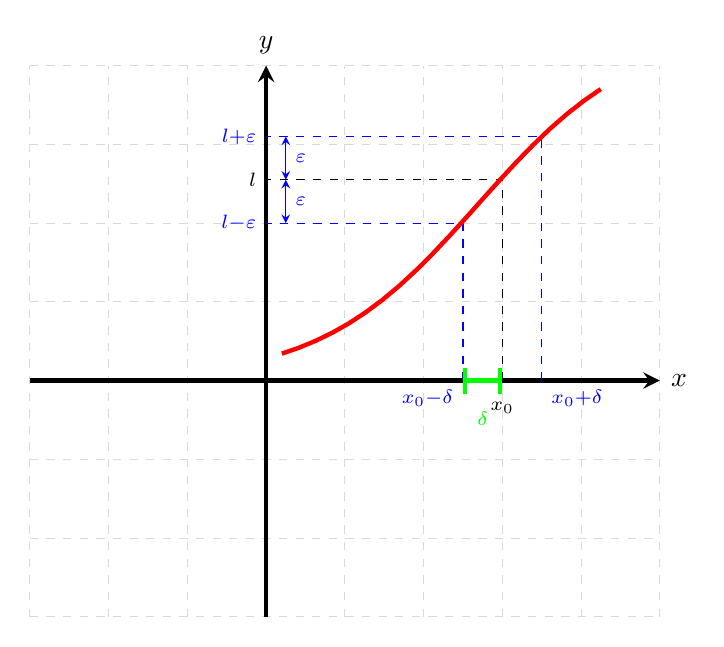
\begin{tikzpicture}[>=stealth]
        % grid and Axis
        \draw[help lines, color=gray!30, dashed] (-3 , -3) grid (5 , 4);
    \draw[->,ultra thick] (-3 , 0) -- (5 , 0) node[right]{$x$}; 
    \draw[->,ultra thick] (0 , -3) -- (0, 4) node[above]{$y$}; 
    % Bounds and function value
    \draw[dashed,color=blue] (3.5, 0) node[below right]
            {$\scriptstyle x_0+\delta$} -- (3.5 , 3.1) -- (0 , 3.1)
            node[left] {$\scriptstyle l+\varepsilon$}; %Upper
    \draw[dashed,] (3  , 0) node[below = 1.5 mm] 
            {$\scriptstyle x_0$} -- (3 , 2.55) -- (0 , 2.55)
            node[left] {$\scriptstyle l$}; % l
    \draw[dashed,color=blue] (2.5 ,  0) node[below left]
            {$\scriptstyle x_0-\delta$} -- (2.5 , 2.0) -- (0 , 2.0)
            node[left] {$\scriptstyle l-\varepsilon$}; % Lower
    \draw[ultra thick,red,domain=-1.8 : 2.25 , samples = 20] {} 
            plot ((\x + 2 , {exp(\x + 1.5)/(2 +  exp(\x)}); % f(x)
    % Annotations
    \draw [|-|, ultra thick, green ] (2.5 , 0) -- (3.0 , 0) 
        node[midway, below = 2.50mm]{$\scriptstyle \delta$}; 
    \draw [<-> , thin , blue] (0.25 , 2.55) -- (0.25 , 3.1)
        node[midway, right] {$\scriptstyle \varepsilon$}; % Upper Arrow
    \draw [<-> , thin , blue] (0.25 , 2) -- (0.25 , 2.55)
            node[midway, right] {$\scriptstyle \varepsilon$}; % Lower Arrow     
    \end{tikzpicture}
\end{center}
\end{tcolorbox}

\item Let $f: D \subseteq \mathbb{R}^2 \longrightarrow \mathbb{R}$ be a two-variable, real-valued function that is differentiable on the domain $D$. Discuss the five step process for constructing the partial derivative of $f$ with respect to $x$. In particular:
\begin{enumerate}[label=\alph*)]
\item Discuss each of the five steps used to derive the limit definition of the partial derivative in slope notation given by
\[
f_x(a, b)=\lim _{x \rightarrow a} \frac{f(x, b)-f(a, b)}{x-a}
\]
Make sure to explicitly describe this concept geometrically and refer back to lines that exist in the intersection between the surface $z=f(x, y)$ and the plane $y=b$.
 \begin{tcolorbox}[%
    enhanced, 
    breakable,
    frame hidden,
    overlay broken = {
        
        (frame.north west) rectangle (frame.south east);},
    ]

  \end{tcolorbox}

\item  Explain, in detail, how this limit definition of $f_x(a, b)$ relates to Path 1 for taking multivariable limits from Lesson 8.
 \begin{tcolorbox}[%
    enhanced, 
    breakable,
    frame hidden,
    overlay broken = {
        
        (frame.north west) rectangle (frame.south east);},
    ]

  \end{tcolorbox}

\item  Using the proper algebraic substitution, create the limit definitions of the partial derivatives in derivative notation given by
\[
f_x(a, b)=\lim _{h \rightarrow 0} \frac{f(a+h, b)-f(a, b)}{h}
\]
 \begin{tcolorbox}[%
    enhanced, 
    breakable,
    frame hidden,
    overlay broken = {
        
        (frame.north west) rectangle (frame.south east);},
    ]

  \end{tcolorbox}
\end{enumerate}

\item 4. Let $f: D \subseteq \mathbb{R}^2 \longrightarrow \mathbb{R}$ be a two-variable, real-valued function given by
$$
f(x, y)=x^3+x^2 y^3-2 y^2
$$
\begin{enumerate}[label=\alph*)]
\item Find $f_x(x, y)$ and use this result to calculate $f_x(2,1)$.
 \begin{tcolorbox}[%
    enhanced, 
    breakable,
    frame hidden,
    overlay broken = {
        
        (frame.north west) rectangle (frame.south east);},
    ]
    To solve this we treat $y$ as a constant and then differentiate with respect to $x$.  Thus,
\begin{align*}
\frac{\partial f}{\partial x} = 3x^2 + 2xy^3
\end{align*}
and
\begin{align*}
  f_x(2,1) &= 3(2)^2+2(2)(1)^3 \\
           &= 12 + 4\\
           &= 16.
\end{align*}
  \end{tcolorbox}

\item Find $f_y(x, y)$ and use this result to calculate $f_y(2,1)$.
 \begin{tcolorbox}[%
    enhanced, 
    breakable,
    frame hidden,
    overlay broken = {
        
        (frame.north west) rectangle (frame.south east);},
    ]
    Here we treat $x$ as a constand and then differentiate with respect to $y$.  Thus,
    \[\frac{\partial f}{\partial y} = 3x^2y^2 - 4y\]
    and
   \begin{align*}
     f_y(2,1) &= 3(2)^2(1)^2-4(1)\\
              &= 12-4\\
              &= 8.
   \end{align*}
  \end{tcolorbox}

\item  Find the higher-order derivatives $f_{x x}, f_{x y}, f_{y x}$, and $f_{y y}$.
 \begin{tcolorbox}[%
    enhanced, 
    breakable,
    frame hidden,
    overlay broken = {
        
        (frame.north west) rectangle (frame.south east);},
    ]
    For all these problems we just find the first order derivative and then use that derivative to find the second.
    So
\begin{align*}
  \frac{\partial f_x}{\partial x} &= 6x + 2y^3 \\
  \frac{\partial f_x}{\partial y} &= 6xy^2 \\
  \frac{\partial f_y}{\partial x} &= 6y^2x\\
  \frac{\partial f_y}{\partial y} &= 6x^2y - 4.
\end{align*}
  \end{tcolorbox}
\end{enumerate}

\item Let $f: D \subseteq \mathbb{R}^2 \longrightarrow \mathbb{R}$ be a two-variable, real-valued function given by
$$
f(x, y)=\sin \left(\frac{x}{1+y}\right)
$$
Find $f_x(x, y)$ and $f_y(x, y)$.
\begin{tcolorbox}[%
    enhanced, 
    breakable,
    frame hidden,
    overlay broken = {
        
        (frame.north west) rectangle (frame.south east);},
    ]
  To solve this, we can use the chain rule.  Thus,
\begin{align*}
  \frac{\partial f}{\partial x} &= \frac{\partial}{\partial x} \sin \left( \frac{x}{1+y} \right)\\
                                &= \cos\left(\frac{x}{1+y}\right) \cdot \frac{1}{1+y}
\end{align*}
and
\begin{align*}
  \frac{\partial f}{\partial y} &= \frac{\partial}{\partial y} \sin \left( \frac{x}{1+y} \right)\\
                                &= \cos\left( \frac{x}{1+y}\right)  \cdot \frac{\partial}{\partial y}\frac{x}{1 + y}\\
                                &= \cos \left( \frac{x}{1 + y} \right) \cdot \frac{\partial}{\partial y} x(1+y)^{-1}\\
                                &= \cos \left( \frac{x}{1 + y} \right) \cdot x \cdot \frac{\partial}{\partial y}(1 + y)^{-1}\\
                                &= \cos \left( \frac{x}{1 + y} \right) \cdot -x \cdot (1+y)^{-2}\\
                                &= -x\cos \left( \frac{x}{1+y}\right) \left(\frac{1}{1+y}\right)^2.                                 
\end{align*}
  \end{tcolorbox}

\item Let $f: D \subseteq \mathbb{R}^3 \longrightarrow \mathbb{R}$ be a three-variable, real-valued function given by
$$
f(x, y, z)=e^{x y} \cdot \ln (z)
$$
Find $f_x(x, y, z), f_y(x, y, z)$, and $f_z(x, y, z)$.
 \begin{tcolorbox}[%
    enhanced, 
    breakable,
    frame hidden,
    overlay broken = {
        
        (frame.north west) rectangle (frame.south east);},
    ]
\begin{itemize}
\item $f_x(x,y,z)$:
\begin{align*}
  \frac{\partial f}{\partial x} &= \frac{\partial}{\partial x} e^{x y} \cdot \ln (z)\\
                                &= \ln (z) \frac{\partial}{\partial x} e^{xy}\\
                                &= \ln (z) \cdot e^{xy} \cdot y.
\end{align*}

\item $f_y(x,y,z)$:
  \begin{align*}
    \frac{\partial f}{\partial y} &= \frac{\partial}{\partial y} e^{x y} \cdot \ln (z)\\
                                  &= \ln (z) \frac{\partial}{\partial y} e^{xy}\\
                                  &= \n (z) \cdot e^{xy} \cdot x
  \end{align*}

\item $f_z(x,y,z)$:
\begin{align*}
  \frac{\partial f}{\partial z} &= \frac{\partial}{\partial z} e^{x y} \cdot \ln (z)\\
                                &=e^{xy} \frac{\partial}{\partial z} \ln (z)\\
                                &=e^{xy}\cdot \frac{1}{z}\\
                                &=\frac{e^{xy}}{z}
\end{align*}
\end{itemize}
  \end{tcolorbox}

\item Let $f: D \subseteq \mathbb{R}^3 \longrightarrow \mathbb{R}$ be a three-variable, real-valued function given by
$$
f(x, y, z)=3 x y \arcsin (y z)
$$
Find $f_x(x, y, z), f_y(x, y, z)$, and $f_z(x, y, z)$.
 \begin{tcolorbox}[%
    enhanced, 
    breakable,
    frame hidden,
    overlay broken = {
        
        (frame.north west) rectangle (frame.south east);},
    ]
    Let's first find $f_x(x,y,z)$:
    \begin{align*}
      \frac{\partial f}{\partial x} &= \frac{\partial}{\partial x} 3xy\arcsin (yz) \\
                                    &=3y\arcsin (yz) \cdot 1\\
                                    &=3y\arcsin (yz).
    \end{align*}
    The next easiest is to find $f_z(x,y,z)$:
 \begin{align*}
   \frac{\partial f}{\partial z} &= \frac{\partial}{\partial z} 3xy\arcsin (yz) \\
                                 &= 3xy \frac{\partial}{\partial z} \arcsin (yz) \\
                                 &= \frac{3xy}{\sqrt{1-(yz)^2}} \cdot  \frac{\partial}{\partial z} (yz)\\
                                 &= \frac{3xy}{\sqrt{1-(yz)^2}} \cdot  y \frac{\partial}{\partial z} (z) \\
                                 &= \frac{3xy}{\sqrt{1-(yz)^2}} \cdot  y.
 \end{align*}
 We can use the power rule which states $\frac{d}{d x}[f(x) g(x)]=f(x) g^{\prime}(x)+f^{\prime}(x) g(x)$ to get $f_y(x,y,z)$:
 \begin{align*}
   \frac{\partial f}{\partial y} &= \frac{\partial}{\partial y} 3xy\arcsin (yz) \\
                                 &= 3x \frac{\partial}{\partial y}y \arcsin (yz)\\
                                 &= 3x((y \cdot \frac{1}{\sqrt{1-(yz)}} \cdot z) + \frac{1}{\arcsin (yz)})
 \end{align*}
  \end{tcolorbox}

\item Consider the following relation
$$
x^3+y^3+z^3+6 x y z=1
$$
Assume that $z=z(x, y)$ and use implicit differentiation to find $\frac{\partial z}{\partial x}$ and $\frac{\partial z}{\partial y}$.
 \begin{tcolorbox}[%
    enhanced, 
    breakable,
    frame hidden,
    overlay broken = {
        
        (frame.north west) rectangle (frame.south east);},
    ]

  \end{tcolorbox}
\end{enumerate}

\stepcounter{section}

\section{Directional Derivative}\label{sec:directional-derivative}
\begin{enumerate}
\item Calculating and interpreting the Directional Derivative
  \begin{enumerate}[label=\alph*)]
  \item Derive the limit definition for directional derivative. Make explicit connections between this limit definition and the limit definition of the ordinary derivative. Explain how these definitions utilize a limiting process to transform the slope of a secant line into the slope of a tangent line at a particular point.
\begin{tcolorbox}[%
    enhanced, 
    breakable,
    frame hidden,
    overlay broken = {
        
        (frame.north west) rectangle (frame.south east);},
    ]
  Let's say that we have a function with one input and one output; that is, from $f : D \subseteq \mathbb{R} \rightarrow \mathbb{R}$.  When we find the derivative we want to see how a slight nudge of the input affects the output.
\begin{center}
\includegraphics[width=7cm]{17.png}
\end{center}
We want to find the ratio between $\Delta y$ and $\Delta x$ as $\Delta x$ approaches 0. Written more formally:
\[\lim_{h \rightarrow 0} \frac{f(x + h) - f(x)}{h}.\]
Imagine that instead of going from the number line to the number line, we are going from $\mathbb{R}^2$ to the number line. To see how a change in input affects our output we have used partial derivatives.  That is, we would hold $y$ constant and change $x$ and see how that affected the output, and do the same with holding $x$ constant and changing $y$.
\begin{center}
\includegraphics[width=7cm]{18.png}
\end{center}But more on this later.  There is no reason why we can't think about how a slight nudge along a different path affects the output of $f$.
\begin{center}
\includegraphics[width=7cm]{20.png}
\end{center}
Let $\vec{a}$ be our starting point, $\vec{w}$ be the direction we will nudge the input and $\Delta f$ be the resulting change in the output after moving $\|\vec{w}\|_2$ in direction of $\vec{w}$.  To utilize the knowledge gained from the ordinary derivative, lets create a new graph, with the $y$ axis represent $f$, the output of the function, and the $x$ axis contain the amount moved in the direction of $\vec{w}$.
\begin{center}
  \includegraphics[width=7cm]{21.jpeg}
\end{center}
Thus, we can convert this secant line to a tangent line by letting $h$ approach 0.  Thus
\[D_{\vec{w}}f(\vec{a}) = \lim_{h \rightarrow 0} \frac{f(\vec{a} + h\vec{w} - f(\vec{a}))}{h}.\]
\end{tcolorbox}

\item Relate the limit definition of the directional derivative to the limit definition of partial derivatives. In particular, find the direction vector $\mathbf{u}$ such that
$$
D_{\mathbf{u}} f(a, b)=f_x(a, b) \quad \text { or } \quad D_{\mathbf{u}} f(a, b)=f_y(a, b)
$$
\begin{tcolorbox}[%
    enhanced, 
    breakable,
    frame hidden,
    overlay broken = {
        
        (frame.north west) rectangle (frame.south east);},
    ]
Well, we can express the limit definition of partial derivatives using vectors.  To do this we just move along the path of on of our basis vectors:
\[\frac{\partial f}{\partial x} = \lim_{h \rightarrow 0} \frac{f(\vec{a} + h\hat{\imath}) - f(\vec{v})}{h}\]
where $\vec{a}$ is the starting point and $\hat{\imath}$ is the unit vector in the direction of the $x$ axis.
\end{tcolorbox}

\item  Derive, using the multivariable chain rule, the dot product formula for the directional derivative.
  \begin{tcolorbox}[%
    enhanced, 
    breakable,
    frame hidden,
    overlay broken = {
        
        (frame.north west) rectangle (frame.south east);},
    ]

  \end{tcolorbox}

\item Use the cosine formula for the dot product and the dot product formula for the directional derivative to explain why the direction of the gradient is the direction steepest ascent. Interpret this result as it relates to the given surfaces.
  \begin{tcolorbox}[%
    enhanced, 
    breakable,
    frame hidden,
    overlay broken = {
        
        (frame.north west) rectangle (frame.south east);},
    ]
    Recall the cosine formula for the dot product
    \[\vec{A} \cdot \vec{B} = \|A\|_2\|B\|_2\cos \theta\]
    and the dot product formula for derictional derivative
    \[D_{\vec{u}}f = \nabla f \cdot \vec{u}\]
    where $\nabla f = \langle \frac{\partial f}{\partial x}, \frac{\partial f}{\partial y} \rangle $.
    A question arises, why is the vector $\nabla f$ the direction of steepest ascent?  Well, recall that the directional derivative $D_{\vec{u}}f(\vec{a})$ represents the rate at which function $f$ changes when moving through $\vec{a}$ in the direction of $\vec{u}$. Thus, the direction of steepest ascent is the direction $\vec{u}$ that maximizes the function $D_{\vec{u}}f(\vec{a})$ where $\|\vec{u}\|_2 = 1$.  Thus, we need to find the direction $\vec{u}$ in which this is the case.
    Thus:
    \begin{align*}
      \max (D_{\vec{u}}f(\vec{a})) &= \max (\nabla f  \cdot \vec{u})\\
                                   &= \max (\| \nabla f\|_2 \cdot \| \operatorname{Proj}_{\nabla f}(\vec{u}))\|_2 \\
                                   &= \max (\| \nabla f\|_2 \cdot \| \|\vec{u}\|_2 \cos \theta \hat{\nabla f} \|_2)\\
                                   &= \max (\| \nabla f \|_2 \cdot \|\vec{u} \cos \theta \|_2)\\
                                   &= \max (\| \nabla f \|_2 \cdot \| \cos \theta \|_2).
    \end{align*}
Since cosine oscilates between $-1$ and $1$, the function will max when cosine is equal to 1, and thus $\theta = 0$.  Therefore, $\vec{u}$ is in direction of $\nabla f$ and so $\nabla f$ returns path of greatest ascent.  
\end{tcolorbox}
  \end{enumerate}
\item The Gradient and Level Curves The level curves to the surface $z=x^2+y^2$ are circles in $\mathbb{R}^2$ centered at the origin. Consider each of the following input points:
\begin{enumerate}[label=\Alph*)]
\item $P(3,-2)$
\item $P(-2,-1)$
\item  $P(-5,12)$
\end{enumerate}
Use this explicit equation for the elliptic paraboloid and the given points to do the following:
\begin{enumerate}[label=\roman*.]
\item Graph the contour and level curve associated with each point.
  \begin{tcolorbox}[%
    enhanced, 
    breakable,
    frame hidden,
    overlay broken = {
        
        (frame.north west) rectangle (frame.south east);},
    ]
    For point $A$, $z = 9 + 4 = 13$, for point $B$, $z = 4 + 1 = 5$, and for point $C$, $z = 25 + 144 =169$.  Thus, we get the following graphs:
\begin{center}
\includegraphics[width=13cm]{22.jpeg}
\end{center}
\end{tcolorbox}

\item Determine the gradient vector at each input point.
  \begin{tcolorbox}[%
    enhanced, 
    breakable,
    frame hidden,
    overlay broken = {
        
        (frame.north west) rectangle (frame.south east);},
    ]
Here, we just have to find the partial derivatives of $f$, and plug in our values for $x$ and $y$.  We see that
\begin{align*}
  \nabla f &= \langle \frac{\partial f}{\partial x}, \frac{\partial f}{\partial y} \rangle \\
           &= \langle 2x, 2y \rangle.
\end{align*}
Therefore
\begin{align*}
  \nabla f(3, -2) &= \langle 6, -4 \rangle \\
  \nabla f(-2,-1) &= \langle -4, -2 \rangle \\
  \nabla f(-5,12) &= \langle -10, 24 \rangle .
\end{align*}
\end{tcolorbox}

\item Graph the gradient vector on the level curves from part i. assuming that the tail of each vector is the given point $P$.
\begin{tcolorbox}[%
    enhanced, 
    breakable,
    frame hidden,
    overlay broken = {
        
        (frame.north west) rectangle (frame.south east);},
    ]
\begin{center}
\includegraphics[width=5cm]{23.png}
\end{center}
\end{tcolorbox}

\item $\text { Find a parametric equation for the tangent line to the level curve at each point } P$.
\begin{tcolorbox}[%
    enhanced, 
    breakable,
    frame hidden,
    overlay broken = {
        
        (frame.north west) rectangle (frame.south east);},
    ]
  Instead of solving for the specific case, let's solve for the generic and use this general form to solve our specific cases.  Recall that to get the equation of a line we need a point and a direction.  Let's assume we are given the point $P(p_1, p_2)$ on our level curve and we want to find the tangent line at that point.  Well, we have a point now we just need a direction.  But we know that the line of steepest ascent is orthogonal to the tangent line, so, our direction is $\langle \frac{\partial f}{\partial y}, -\frac{\partial f}{\partial x} \rangle $.  Thus, the tangent line of our level curve at point $P(p_1, p_2)$ takes the form
  \[l(t) = \langle p_1, p_2 \rangle  + t \langle \frac{\partial f}{\partial y}, -\frac{\partial f}{\partial x} \rangle .\]
  Substituting the partial derivatives of our equation $f(x,y) = x^2 + y^2$ we get
  \[f(t) = \langle x,y \rangle + t \langle 2y, -2x \rangle\]
  and by inspection we see that the equation of tangent at point $A$ is $f(t) = \langle 3, -2 \rangle  + t \langle -4, -6 \rangle$ at point $B$ is $f(t) = \langle -2, -1 \rangle  + t \langle -2, 4 \rangle$ and atpoint $C$ is $f(t) = \langle -5, 12 \rangle  + t \langle 24, 10 \rangle$.  Adding these tangent lines to our graph of level curves we get:
\begin{center}
\includegraphics[width=13cm]{24.png}
\end{center}
\end{tcolorbox}
\end{enumerate}

\item The Gradient and Steepest Descent Consider the paraboloid
$$
f(x, y)=16-\frac{x^2}{4}-\frac{y^2}{16},
$$
Let $P$ be the point on a given level curve of $f(x, y)$, as described in each part below. Compute the slope of the line tangent to the level curve at $P$ and verify that the tangent line is orthogonal to the gradient at that point.
\begin{enumerate}[label=\alph*)]
\item Level curve $f(x, y)=0$ including point $P(0,16)$
\begin{tcolorbox}[%
    enhanced, 
    breakable,
    frame hidden,
    overlay broken = {
        
        (frame.north west) rectangle (frame.south east);},
    ]
  We will first find the partial derivative of $f(x,y)$ and then use the general form of our equation to get the slope of the tangent line.  We see that
\begin{align*}
  \frac{\partial f}{\partial x} &= 0 - \frac{1}{4}(2)x - 0\\
                                &= - \frac{2}{4}x \\
                                &= - \frac{1}{2}x
\end{align*}
and
\begin{align*}
 \frac{\partial f}{\partial y} &= 0 - 0 -\frac{1}{16}(2)y\\
                                &= -\frac{2}{16}y \\
                                &= - \frac{1}{8}y.
\end{align*}
Therefore the direction vector of the tangent line orthogonal to the gradient is $ \langle -\frac{1}{8}y, \frac{1}{2}x \rangle $, or for point $P(0,16)$, $\langle -2, 0 \rangle $.  Since there is no change in $y$ no matter how much $x$ is changed, the slope is 0.  Or written another way
\begin{align*}
  \text{ Slope } &= \frac{\text{rise} }{\text{run}} \\
                 &= \frac{0}{-2}\\
                 &= 0.
\end{align*}
\end{tcolorbox}

\item Level curve $f(x, y)=12$ including point $P(4,0)$
\begin{tcolorbox}[%
    enhanced, 
    breakable,
    frame hidden,
    overlay broken = {
        
        (frame.north west) rectangle (frame.south east);},
    ]
  Direction of tangent line is:
  \begin{align*}
    \langle -\frac{1}{8}y, \frac{1}{2}x \rangle &= \langle -\frac{1}{8}(0), \frac{1}{2}(4) \rangle \\
                                                &= \langle 0, 2 \rangle.
  \end{align*}
  Thus we see that the tangent line is moving in a straight vertical line, so the slope is undefined. Or expressed mathematically
  \begin{align*}
  \text{ Slope } &= \frac{\text{rise} }{\text{run}} \\
                 &= \frac{2}{0}\\
                 &= \text{undefined} .
\end{align*}
\end{tcolorbox}

\item Level curve $f(x, y)=12$ including point $P(2 \sqrt{3}, 4)$
\begin{tcolorbox}[%
    enhanced, 
    breakable,
    frame hidden,
    overlay broken = {
        
        (frame.north west) rectangle (frame.south east);},
    ]
  Direction of tangent line is:
  \begin{align*}
    \langle -\frac{1}{8}y, \frac{1}{2}x \rangle &= \langle -\frac{1}{8}(4), \frac{1}{2}(2 \sqrt{3}) \rangle \\
                                                &= \langle -\frac{1}{2}, \sqrt{3} \rangle.
  \end{align*}
  Thus the slope is $-2 \sqrt{3}$.
\end{tcolorbox}
\end{enumerate}
\end{enumerate}

\section{Tangent Planes and Linearizations}\label{sec:tangent-planes}
\begin{enumerate}
\item Derive the equation for a tangent plane Suppose we are given a surface in $\mathbb{R}^3$ that is defined implicitly as a level surface using equation
$$
F(x, y, z)=0
$$
where the function $F: D \rightarrow \mathbb{R}$ is differentiable for all domain values in $D \subseteq \mathbb{R}^3$.
\begin{enumerate}[label=\alph*)]
\item  Derive the equation for the tangent plane to the level surface at point $(a, b, c)$ on this surface. Make sure to mention the geometric interpretation of the gradient vector with respect to the tangent plane.
  \begin{tcolorbox}[%
    enhanced, 
    breakable,
    frame hidden,
    overlay broken = {
        
        (frame.north west) rectangle (frame.south east);},
    ]
    Let's first recall the vector valued gradient function $\nabla f(x,y)$, $\nabla f: \mathbb{R}^2 \rightarrow \mathbb{R}^2$.  This function returns the vector whose components are the partial derivatives of $f$, $\langle \frac{\partial f}{\partial x}, \frac{\partial f}{\partial y} \rangle$ whose direction is that of steepest ascent of $f$.  What is exactly meant by ``direction of steepest ascent''?.  Let's say that we have the function $f(x,y) = x^2 + y^2$.  Then we have a function $f: \mathbb{R}^2 \rightarrow \mathbb{R}$, and so to draw the graph of $f$ we need three axis, two for the inputs ($x,y$), and one for the output, $z$. Notice though, that the gradient vector of $f$, $\nabla f$, lies in $\mathbb{R}^2$ and so, the ``direction of steepest ascent'' refers to the direction at point $x,y$ on the level curve of $f$ that points in the direction of the shortest path to the next level curve.  A picture may help:
\begin{center}
\includegraphics[width=6cm]{25.png}
\end{center}
Notice that we have the gradient of $f$ that lies in the domain space of $f$, and is tangent to the level curve.  Why is this? This is because the shortest path between two parallel lines is a line orthoganal to the two.  Also note, that as the change in $f$ decreases (distance between level curves decreases) the two level curves will appear more and more parallel, and more and more like straight lines.  This is the intuition behind why the gradient is orthogonal to the level curve.\\\\
Now lets say we have a function $w = f(x,y,z)$, where $w$ is a real number.  Then we have $f: \mathbb{R}^3 \rightarrow R$.  This function is not possible to draw, since we would need 4 axis, three for the inputs and one for the outputs.  But what we can draw, is the level surface.  What is a level surface?  It is the three dimensional surface such that all points on the surface equal some constant $c$.  This is something that we can draw.  In this problem for example, we have the level surface $F(x,y,z) = 0$ of some function $f(x,y,z) = w$.  The gradient of $f$, $\nabla f$, will be orthogonal to the level surface $F$.  Why is this?  The same reasoning that applied to level curves, applies to level surfaces.  The direction of steepest ascent is the direction of the next closest level surface.  But as we make the next closest level surface closer and closer, and zoom in more and more, the two surfaces will become indistinguishable from parallel planes, and the shortest distance between two parallel planes is along a path orthogonal to the two planes.\\\\
Now to get back to the original question; we want to find the tangent plane to a level surface that lies in $\mathbb{R}^3$ at some point $P_0(a,b,c)$.  Recall the equation of a vector
\[\vec{n} \cdot \overrightarrow{P_0P} = 0.\]
We have the two required pieces of information a point on the plane and a vector normal to the plane.  The point is $P_0 = (a,b,c)$ and the normal vector is the gradient at point $P_0$: $\left\langle\left.\frac{\partial f}{\partial x}\right|_{P_{0}},\left.\frac{\partial f}{\partial y}\right|_{P_0},\left.\frac{\partial f}{\partial z}\right|_{P_0}\right\rangle$.  Thus, the equation of of a plane tangent to a level surface at point $P_0$ is
\[\left\langle\left.\frac{\partial f}{\partial x}\right|_{P_{0}},\left.\frac{\partial f}{\partial y}\right|_{P_0},\left.\frac{\partial f}{\partial z}\right|_{P_0}\right\rangle \cdot \overrightarrow{P_0P} = 0.\]
  \end{tcolorbox}

\item Suppose we have a surface in $\mathbb{R}^3$ defined by function $z=f(x, y)$ for differentiable function $f$. Derive the equation for a tangent plane to this surface at the point $(a, b, f(a, b))$ by relating this situation back to your work in part A.
  \begin{tcolorbox}[%
    enhanced, 
    breakable,
    frame hidden,
    overlay broken = {
        
        (frame.north west) rectangle (frame.south east);},
    ]
    Here we want to a tangent plane of $f$ at some point.  But we have a problem, the gradient vector lies in the domain space of $f$, which in this case is $\mathbb{R}^2$ and we need a gradient vector in $\mathbb{R}^3$.  We can perform some algabraic manipulation so that we have a level surface in $\mathbb{R}^3$:
    \begin{align*}
      z &= f(x,y)\\
      0 &= f(x,y) - z.
    \end{align*}
    Now we have a function $F(x,y,z) = F(x,y,f(x,y)) = 0$ of a level surface in $\mathbb{R}^3$.  The gradient at of $F$ at point $P_0$ is:
    $\left\langle\left.\frac{\partial f}{\partial x}\right|_{P_{0}},\left.\frac{\partial f}{\partial y}\right|_{P_0},\left.\frac{\partial f}{\partial z}\right|_{P_0}\right\rangle$.  Notice though that $F(x,y,z) = f(x,y) - z$, and finding the partial derivative of $F$ with respect to $z$ we get:
    \begin{align*}
      \frac{\partial F}{\partial z} &= \frac{\partial}{\partial z} f(x,y) - z\\
                                    &= \frac{\partial}{\partial z} -z\\
                                    &= -1 \frac{\partial}{\partial z} z \\
                                    &= -1.
    \end{align*}
    Then, by substitution we have
\begin{align*}
  \nabla F(a,b, f(a,b)) &= \left\langle\left.\frac{\partial f}{\partial x}\right|_{P_{0}},\left.\frac{\partial f}{\partial y}\right|_{P_0},\left.\frac{\partial f}{\partial z}\right|_{P_0}\right\rangle \\
  &= \left\langle\left.\frac{\partial f}{\partial x}\right|_{P_{0}},\left.\frac{\partial f}{\partial y}\right|_{P_0}, -1\right\rangle
\end{align*}
where $P_0 = (a, b, f(a,b))$.  Thus, the equation of a plane tangent to the the surface $z = f(x,y)$ at point $P_0 = (a, b, f(a,b))$ is:
\[\left\langle\left.\frac{\partial f}{\partial x}\right|_{P_{0}},\left.\frac{\partial f}{\partial y}\right|_{P_0}, -1\right\rangle \cdot \overrightarrow{P_0P}.\]
\end{tcolorbox}
\end{enumerate}
\item Consider the implicit relation for the ellipsoid defined by equation
$$
\frac{x^2}{9}+\frac{y^2}{25}+z^2-1=0 .
$$
Using this equation, please do the following:
\begin{enumerate}[label=\alph*)]
\item Find the equation for the tangent plane to the ellipsoid at the point $\left(0,4, \frac{3}{5}\right)$
  \begin{tcolorbox}[boxrule=0pt, frame empty]
    Using the formula above, we have the equation for the tangent plane to the ellipsoid at point $P_0 = (0,4, \frac{3}{5})$ is:
\begin{align*}
\left\langle\frac{2}{4} x, \frac{2}{25} y, 2 z\right\rangle \cdot \overrightarrow{P_0 P} &=0 \\
\left\langle 0, \frac{8}{25}, \frac{6}{5}\right\rangle \cdot \overrightarrow{(0,4, \frac{3}{5})(x, y, z)} &=0 \\
\left\langle 0, \frac{8}{25}, \frac{6}{5}\right\rangle \cdot\left\langle x, y-4, z-\frac{3}{5}\right\rangle &=0 \\
0 x+\frac{8}{25} y+\frac{6}{5} z-\frac{32}{25}-\frac{18}{25} &=0 \\
0 x+\frac{8}{25} y+\frac{6}{5} z-\frac{50}{25} &=0 \\
\frac{8}{25} y+\frac{6}{5} z-2 &=0
\end{align*} 
  \end{tcolorbox}

\item Find any point(s) on the ellipsoid with a horizontal tangent plane.
  \begin{tcolorbox}[boxrule=0pt, frame empty]
    A Horizontal tangent plane will have a normal vector
    \[\vec{n} = \langle 0, 0, c \rangle \]
    where $c$ is some constant.  Thus, we need to find point(s) $P$ such that $\nabla F(x,y,z) = \langle 0,0, c \rangle $.  We see that the normal vector to our plane at point $(x,y,z)$ is $\langle \frac{2}{9}x, \frac{2}{25} y, 2z \rangle $.  Setting $x = y = 0$ in our equation we see that our ellipsoid will have a horizontal tangent plane at points $(0,0, 1)$ and $(0, 0, -1)$.
  \end{tcolorbox}
\end{enumerate}

\item Find the equation of the tangent plane to the elliptic paraboloid defined by the explicit equation
$$
z=f(x, y)=2 x^2+y^2
$$
at the point $(1,1,3)$.
\begin{tcolorbox}[boxrule=0pt, frame empty]
We have the level surface $F(x,y,z) = 2x^2+y^2-z$.
    Let's first find a normal vector $\vec{n}$:
    \begin{align*}
\vec{n} &=\left\langle\left.\frac{\partial F}{\partial x}\right|_p,\left.\frac{\partial F}{\partial y}\right|_p,-1\right\rangle \\
&=\left\langle\left. 4 x\right|_p,\left.2 y\right|_{p,}-1\right\rangle \\
&=\langle 4(1), 2(1),-1\rangle \\
&=\langle 4,2,-1\rangle.
    \end{align*}
    Thus, the plane tanget to $z = f(x,y)$ at point $P_0 = (1,1,3)$ is:
\begin{align*}
0&=\vec{n} \cdot \overrightarrow{P_0 P} \\
&=\langle 4,2,-1\rangle \cdot \overrightarrow{(1,1,3)(x, y, z)} \\
&=\langle 4,2,-1\rangle \cdot\langle x-1, y-1, z-3\rangle \\
&=4 x+2 y-z-4-2+3 \\
&=4 x+2 y-z-6+3 \\
&=4 x+2 y-z-3.
\end{align*} 
\end{tcolorbox}

\item Define a two-variable, real-valued function given by
$$
f(x, y)=\frac{5}{x^2+y^2}
$$
Find the linear approximation to $f$ at the point $(-1,2,1)$.
  \begin{tcolorbox}[%
    enhanced, 
    breakable,
    frame hidden,
    overlay broken = {
        
        (frame.north west) rectangle (frame.south east);},
    ]
    Given $z = f(x,y)$, how can we find a linear approximation such that $L(x,y) \approx f(x,y)$ for values near some $(a,b)$.  Well, note that the equation of a plane is linear, and that a tangent plane at point $P_0$ approxomates a level surface for values $(x,y,z)$ close to $P_0$.  But, we are given a function with two inputs.  So, what we will do is first create a level surface $F(x,y,z) = 0$ find the tangent plane at some point $(a,b, f(a,b))$ and then create our linear approximation $L(x,y)$ by setting $L(x,y) = z$.  \\\\
    Let $P_0 = (a,b, f(a,b))$ and $\vec{n} = \langle \frac{\partial F}{\partial x}, \frac{\partial F}{\partial y}, -1 \rangle$.  Thus,
\begin{align*}
0 &=\vec{n} \cdot \overrightarrow{P_0 P} \\
&=\left\langle\left.\frac{\partial F}{\partial x}\right|_{P_0},\left.\frac{\partial F}{\partial y}\right|_{P_0}-1\right\rangle \cdot\langle x-a, y-b, z-f(a, b)\rangle \\
&=\left.\frac{\partial F}{\partial x}\right|_{P_0}(x)+\left.\frac{\partial F}{\partial y}\right|_0(y)-z-\left.\frac{\partial F}{\partial x}\right|_{P_0}(a)-\left.\frac{\partial F}{\partial y}\right|_{p_0}(b)+f(a, b) \\
z &=\left.F_x\right|_{P_0}(x-a)+\left.F_y\right|_{P_0}(y-b)+f(a, b)
\end{align*}
and so
\[L(x,y) = \left.F_x\right|_{P_0}(x-a)+\left.F_y\right|_{P_0}(y-b)+f(a, b).\]
\\\\
Using this equation, we see that
\begin{align*}
L(x, y) &=\frac{10}{25}(x+1)-\frac{20}{25}(y-2)+1 \\
&=\frac{10}{25} x+\frac{20}{25} y+\frac{50}{25}+1 \\
&=\frac{2}{5} x+\frac{4}{5} y+3.
\end{align*}
  \end{tcolorbox}
\end{enumerate} 

\section{Multivariable Optimization}\label{sec:multivariable-optimization}
\begin{enumerate}
\item Review of the method of completing the squares
  \begin{enumerate}[label=\alph*)]
\item  Write each of the following perfect squares as the equivalent trinomial in the form $x^2+2 b x+c$. Show your steps. Make sure to specifically find the values of the coefficients $b$ and $c$.
\begin{enumerate}[label=\roman*.]
\item $(x-4)^2$
  \begin{tcolorbox}[boxrule=0pt, frame empty]
\begin{align*}
(x-4)^2 &=(x-4)(x-4) \\
&=x^2-4 x-9 x+16 \\
&=x^2-8 x+16
\end{align*}
$b = -4, c = 16$
  \end{tcolorbox}
\item $(x+3)^2$
  \begin{tcolorbox}[boxrule=0pt, frame empty]
\begin{align*}
(x+3)^2 &=(x+3)(x+3) \\
&=x^2+3 x+3 x+9 \\
&=x^2+6 x+9
\end{align*}
$b = 3, c = 9$
  \end{tcolorbox}
\item $(x+11)^2$
  \begin{tcolorbox}[boxrule=0pt, frame empty]
$$
\begin{aligned}
(x+11)^2 &=(x+11)(x+11) \\
&=x^2+11 x+11 x+121 \\
&=x^2+22 x+121
\end{aligned}
$$
$b = 11, c = 121$.
  \end{tcolorbox}
\item $\left(x-\frac{7}{2}\right)^2$
  \begin{tcolorbox}[boxrule=0pt, frame empty]
$$
\begin{aligned}
\left(x-\frac{7}{2}\right)^2 &=\left(x-\frac{7}{2}\right)\left(x-\frac{7}{2}\right) \\
&=x^2-\frac{7}{2} x-\frac{7}{2} x+\frac{49}{4} \\
&=x^2-\frac{14}{2} x+\frac{49}{4}
\end{aligned}
$$
$b = -\frac{7}{2}, c = \frac{49}{4}$
  \end{tcolorbox}
\end{enumerate}

\item For each of the problems above, write the equivalent expressions in the form
$$
(x+d)^2=x^2+2 b x+c
$$
Please specifically identify the values of the coefficients $d, b$, and $c$.
\begin{enumerate}[label=\roman*.]
\item $(x-4)^2$
  \begin{tcolorbox}[boxrule=0pt, frame empty]
$d = -4, b = -4, c = 16$.
  \end{tcolorbox}
\item $(x+3)^2$
  \begin{tcolorbox}[boxrule=0pt, frame empty]
$d = 3, b = 3, c = 9$.
  \end{tcolorbox}
\item $(x+11)^2$
  \begin{tcolorbox}[boxrule=0pt, frame empty]
$d = 11, b = 11, c = 121$.
  \end{tcolorbox}
\item $\left(x-\frac{7}{2}\right)^2$
  \begin{tcolorbox}[boxrule=0pt, frame empty]
$d = -\frac{7}{2}, b = -\frac{7}{2}, c = \frac{49}{4}$.
  \end{tcolorbox}
\end{enumerate}

\item Look back on the work you finished in problem 2 above. What pattern do you notice? Specifically, how are the coefficients $d, b$, and $c$ related to each other?
  \begin{tcolorbox}[boxrule=0pt, frame empty]
$d = b$ and $d^2 = b^2 = c$.
  \end{tcolorbox}
\end{enumerate}

\item Review of quadratic functions Consider the standard equation for a quadratic polynomial, given by
$$
f(x)=a x^2+b x+c
$$
Use this general form to answer each of the following problems
\begin{enumerate}[label=\alph*)]
\item What do each of the coefficients $a, b, c \in \mathbb{R}$ do to the graph of this function?
  \begin{tcolorbox}[boxrule=0pt, frame empty]
    Playing with desmos, we see that $a$ changes the ``narrowness'' of parabola.  The greater $a$ is, the more narrow the parabala is.  Also, $a$ is responsible for the concavity of the parabola. When $a$ is positive, the graph is concave up, and when negative it is concave down.  Also, when $a = 0$, the graph is no longer a parabola, but a line.\\\\
Changing $b$ has the effect of moving the vertex along what seems to be the path of a parabola.  We will investigate why this is further below.
  \end{tcolorbox}

\item Use the method of completing the square to derive the quadratic formula.
  \begin{tcolorbox}[%
    enhanced, 
    breakable,
    frame hidden,
    overlay broken = {
        
        (frame.north west) rectangle (frame.south east);},
    ]
    Recall the quadratic formula:
    \[x=\frac{-b \pm \sqrt{b^2-4 a c}}{2 a}.\]
    To derive the quadratic formula we start with the standard form of quadratic equation:

\begin{align*}
  ax^2 + bx + c &= 0 \\
  ax^2 + bx &= -c & & \textit{\textcolor{blue}{Subtrac $c$}}\\
  x^2 + \frac{b}{a}x &= \frac{-c}{a} & & \textit{\textcolor{blue}{Divide by $a$}}\\
  x^2 + \frac{b}{a}x + (\frac{1}{2} \cdot \frac{b}{a})^2 &= \frac{-c}{a} +  (\frac{1}{2} \cdot \frac{b}{a})^2 & & \textit{\textcolor{blue}{Setup to allow completing of square}} \\
  (x + \frac{b}{2a})^2 &= (\frac{b}{2a})^2-\frac{c}{a} & & \textit{\textcolor{blue}{Factor perfect square}}\\
  (x + \frac{b}{2a})^2 &= \frac{b^2}{4a^2}-\frac{c}{a} & & \textit{\textcolor{blue}{Square fraction}}\\
  (x + \frac{b}{2a})^2 &= \frac{b^2}{4a^2}-\frac{4ac}{4a^2} & & \textit{\textcolor{blue}{Get common denominator}} \\
  (x + \frac{b}{2a})^2 &= \frac{b^2-4ac}{4a^2} & & \textit{\textcolor{blue}{Combine fractions}}\\
  x + \frac{b}{2a} &= \sqrt{\frac{b^2-4ac}{4a^2}} & & \textit{\textcolor{blue}{Square root of both sides}}\\
  x + \frac{b}{2a} &= \frac{\sqrt{b^2-4ac}}{2a} & & \textit{\textcolor{blue}{Square root of denominator}}\\
x&=\frac{-b \pm \sqrt{b^2-4 a c}}{2 a} & & \textit{\textcolor{blue}{Isolate $x$}}.
\end{align*}
  \end{tcolorbox}

\item Use the method of completing the square to derive the vertex form of the quadratic function
$$
f(x)=a(x-h)^2+k
$$
Your derivation should include an explicit formula for $h$ and $k$ in terms of $a, b$ and $c$.
  \begin{tcolorbox}[%
    enhanced, 
    breakable,
    frame hidden,
    overlay broken = {
        
        (frame.north west) rectangle (frame.south east);},
    ]
    Going the other way is a lot simpler:
$$
\begin{aligned}
f(x) &=a(x-h)^2+k \\
&=a(x-h)(x-h)+k \\
&=a\left(x^2-2 x h+h^2\right)+k \\
&=a x^2-2 a x h+a h^2+k.
\end{aligned}
$$
Thus since
\[f(x) = ax^2 + bx + c \quad \text{ and } \quad f(x) = a x^2-2 a x h+a h^2+k\]
describe the same curve, we have $h = \frac{b}{-2a}$ and $k = c - \frac{b^2}{4a}$.  Since the vertex of the parabola defined by $f(x) = a(x-h)^2 + k$ is at point $(h, k)$ then by substitution, the vertex lies at $(\frac{b}{-2a}, c - \frac{b^2}{4a})$.  This explains why that if we leave $a$ and $c$ constant and change $b$ the path the path of the changing vertex follows a parabola; $b$ affects the $x$ coordinate linearly and the $y$ coordinate quadratically.  The path that this vertex travels is $y = -ax^2 + c$.  To see this, note:
\begin{align*}
  y &= c - \frac{b^2}{4a} \\
    &= c - \frac{(-2ax)^2}{4a} & & \textit{\textcolor{blue}{$b = -2ax$}}\\
    &=c - \frac{4a^2x^2}{4a} \\
    &= c - ax^2 \\
  &= -ax^2 + c.
\end{align*}
\begin{center}
\includegraphics[width=12cm]{26.png}
\end{center}
  \end{tcolorbox}
\end{enumerate}

\item Derive the second ordinary derivative test Suppose we are given a function $f: D \subseteq \mathbb{R} \longrightarrow \mathbb{R}$ with continuous second derivative on the domain $D$. Let $a \in D$ be a given constant with point $(a, f(a))$ on the graph of our function. .Using this information, please:
\begin{enumerate}[label=\alph*)]
\item State, from memory, the second ordinary derivative test including all three conditions.
  \begin{tcolorbox}[boxrule=0pt, frame empty]
    The second-derivative test is used to test critical points to see if they are local-maxima or local-minima.  If the function is twice differentiable and
\begin{itemize}
\item $f^{\prime \prime}(x) > 0$ then the point is a local minima,
\item $f^{\prime \prime}(x) < 0$ then the point is a local maxima,
\item $f^{\prime \prime}(x) = 0$ then the test is inconclusive.
\end{itemize}
  \end{tcolorbox}

\item Write the equation for the first-order Taylor series approximation $T_1(x)$ of this function at the point $(a, f(a))$. In other words, please write the equation to the tangent line to $f$ at the point $(a, f(a))$. This is known as a local linear approximation of the function $f$ at the point $(a, f(a))$.
  \begin{tcolorbox}[boxrule=0pt, frame empty]
    Recall that for the equation of a line we need a point and a slope.  The point is $(a, f(a))$ and the slope is $f^\prime(a)$.  Thus, we can use the point slope form of equation for a line to get the equation $T_1(x) = y$:
    \begin{align*}
      y - f(a) &= f^\prime(a)(x-a)\\
      y &= f^\prime(a)(x-a) + f(a)\\
      T_1(x) &= f^\prime(a)(x-a) + f(a).
    \end{align*}
  \end{tcolorbox}

\item Write the equation for the second-order Taylor series approximation $T_2(x)$ of this function at the point $(a, f(a))$. In other words, write the equation for the tangent parabola at point $(a, f(a))$. This is known as a local quadratic approximation of the function $f$ at the point $(a, f(a))$.
\begin{tcolorbox}[%
    enhanced, 
    breakable,
    frame hidden,
    overlay broken = {
        
        (frame.north west) rectangle (frame.south east);},
    ]
  We will explore the details of the Taylor Series later, but the quadratic aproximation of a function is
  \[T_2(x)=f(a)+f^{\prime}(a)(x-a)+\frac{f^{\prime \prime}(a)}{2}(x-a)^2.\]
\end{tcolorbox}
\item Explain how the second ordinary derivative test is related to the idea of the tangent line $T_1(x)$ and the tangent parabola $T_2(x)$. In particular, reinterpret the three conditions of the second ordinary derivative test using language about the graphs of these tangent polynomials. For example, what is the slope of the tangent line at a local minimum point? Does the tangent parabola point upwards or downwards at such a minimum? By answering these type of questions for each of the conditions, you will be building a strong geometric interpretation associated with the second ordinary derivative test which you can then use to guide your understanding of the second partial derivative test.
  \begin{tcolorbox}[%
    enhanced, 
    breakable,
    frame hidden,
    overlay broken = {
        
        (frame.north west) rectangle (frame.south east);},
    ]
A local minimum or maximum will happen when the slope of tangent line is zero.  We can see that if the second derivative is negative at $a$ then the quadratic approximation will face downwards and if it is positive it will face upwards.  When the second derivative is zero, our approximation is a horizontal tangent line and this doesn't give us any indication if we are dealing with a local minimum or maximum.  
  \end{tcolorbox}
\end{enumerate}

\item Derive the second partial derivative test. Suppose we are given a function $f: D \subseteq \mathbb{R}^2 \longrightarrow \mathbb{R}$ with continuous second derivative on the domain $D$. Let $(a, b) \in D$ be a given constant with point $(a, b, f(a, b))$ on the graph of our function. Using this information, please:
\begin{enumerate}[label=\alph*)]
\item State, from memory, the second partial derivative test including all four conditions.
  \begin{tcolorbox}[boxrule=0pt, frame empty]
    The second partial derivative test can be used to test critical points (partial derivatives equal zero) to see if a critical point is a local maximum, local minimum, saddle point or inconclusive.
    Given the $2 \times 2$ Hessian Matrix of second partial derivatives:
 \[H(x, y)=\left[\begin{array}{ll}
f_{x x}(x, y) & f_{x y}(x, y) \\
f_{y x}(x, y) & f_{y y}(x, y)
                 \end{array}\right]\]
             and the determinant
             \[D(x, y)=\operatorname{det}(H(x, y))=f_{x x}(x, y) f_{y y}(x, y)-\left(f_{x y}(x, y)\right)^2\]
             then the second partial derivative tells us the following:
\begin{itemize}
\item If $D(a, b)>0$ and $f_{x x}(a, b)>0$ then $(a, b)$ is a local minimum of $f$.
\item If $D(a, b)>0$ and $f_{x x}(a, b)<0$ then $(a, b)$ is a local maximum of $f$.
\item If $D(a, b)<0$ then $(a, b)$ is a saddle point of $f$.
\item If $D(a, b)=0$ then the second derivative test is inconclusive.
\end{itemize}
  \end{tcolorbox}

\item Write the equation for the first-order Taylor series approximation $T_1(x, y)$ of $f$ at point $(a, b, f(a, b))$. In other words, please write the equation to the tangent plane to $f$ at point $(a, b, f(a, b))$. This is known as a local linear approximation of the function $f$ at the point $(a, b, f(a, b))$.
  \begin{tcolorbox}[boxrule=0pt, frame empty]
Recall, that to create a tangent plane of a surface of the equation $f(x,y) = z$, we need to convert our surface into a level surface $F(x,y,z) = f(x,y) -z = 0$ and then get the gradient of this surface ($\nabla F(x,y,z)$).  So, let $F$ be said level surface.  Then to get the equation of our plane we need a point and a direction of that plane.  Our point will be $P_0 = (a,b,f(a,b))$ and the direction of the plane will be determined by the gradient $\left\langle\left.\left.\frac{\partial F}{\partial x}\right|_{P_0,} \frac{\partial F}{\partial y}\right|_{P_0},-1\right\rangle $.  Thus, the equation of the tangent plane is:
    \begin{align*}
      0 &=\vec{n} \cdot \overrightarrow{P_0 P} \\
        &=\left\langle\left.\frac{\partial F}{\partial x}\right|_{P_0},\left.\frac{\partial F}{\partial y}\right|_{P_0},-1\right\rangle \cdot\langle x-a, y-b, z-f(a, b)\rangle \\
        &\left.=F_x(a, b, f(a,b))(x-a)+F_y(a, b, f(a,b))(y-b)-(z-f(a, b))\right\rangle \\
        &=F_x(a, b, f(a,b))(x-a)+F_y(a, b, f(a,b))(y-b)+f(a, b)-z \\
      z &=F_x(a, b, f(a,b))(x-a)+F_y(a, b, f(a,b))(y-b)+f(a, b).
    \end{align*}
    Notice though, that since in the level surface $F$, since $z$ is by itself, the value of $z$ doesn't change the partial derivatives $F_x$ or $F_y$ and thus, we can simplify our equation and only worry about our original equation $f(x,y)$.  Thus,
 \[T_1(x,y) = f_x(a,b)(x-a) + f_y(a,b)(y-b) + f(a,b).\]
  \end{tcolorbox}

\item Write the equation for the second-order Taylor series approximation $T_2(x, y)$ of $f$ at the point $(a, b, f(a, b))$. In other words, write the equation for the tangent quadratic surface at point $(a, b, f(a, b))$. This is known as a local quadratic approximation of the function $f$ at the point $(a, b, f(a, b))$.
  \begin{tcolorbox}[boxrule=0pt, frame empty]
    Since we haven't really gotten to taylor series yet, let's not go into the details of why, but here is the second order taylor series approximation:
    \[f(x, y) \approx Q(x, y)=T_1(x, y)+\frac{f_{x x}(a, b)}{2}(x-a)^2+f_{x y}(a, b)(x-a)(y-b)+\frac{f_{y y}(a, b)}{2}(y-b)^2.\]
  \end{tcolorbox}

\item Combine the fact that we want to look at points on the surface where $\nabla f(x, y)=\mathbf{0}$ with algebra to translate your equation for $T_2(x, y)$ into the form
$$
T_2(x, y)=\frac{1}{2}\left(a x^2+2 b x y+c y^2\right)+k_0 .
$$
In your work, specifically identify the values of $a, b$ and $c$ in terms of the second-order partial derivatives $f_{x x}, f_{y y}$, and $f_{y y}$.
  \begin{tcolorbox}[boxrule=0pt, frame empty]
    Since $\nabla f(x,y) = \vec{0}$, both the first partial derivatives will be zero.  Thus, the only part of $T_1(x,y)$ that remains is $f(a,b)$.  Therefore we have
    \begin{align*}
      f(x, y) \approx &=f(a, b)+\frac{f_{x x}(a, b)}{2}(x-a)^2+f_{x y}(a, b)(x-a)(y-b)+\frac{f_{y y}(a, b)}{2}(y-b)^2\\
      &= \frac{1}{2}(f_{x x}(a, b)(x-a)^2+2f_{x y}(a, b)(x-a)(y-b)+f_{y y}(a, b)(y-b)^2) + f(a,b)
    \end{align*}
    where $a = $
  \end{tcolorbox}

\item Use the method of completing the square to show the following:
$$
a x^2+2 b x y+c y^2=a\left(x-\frac{b}{a} y\right)^2+\frac{a c-b^2}{a} y^2 .
$$
Using this factorization, explain how to determine the behavior of the local quadratic approximation $T_2(x, y)$ based on the values of the coefficients $a$ and $a c-b^2$.
  \begin{tcolorbox}[boxrule=0pt, frame empty]

  \end{tcolorbox}

\item Explain how the second ordinary derivative test is related to the idea of the tangent line $T_1(x)$ and the tangent parabola $T_2(x)$. In particular, reinterpret the three conditions of the second ordinary derivative test using language about the graphs of these tangent polynomials. For example, what is the slope of the tangent line at a local minimum point? Does the tangent parabola point upwards or downwards at such a minimum? By answering these type of questions for each of the conditions, you will be building a strong geometric interpretation associated with the second ordinary derivative test which you can then use to guide your understanding of the second partial derivative test.
  \begin{tcolorbox}[boxrule=0pt, frame empty]

  \end{tcolorbox}
\end{enumerate}

\item Find the points on the plane $x + y + z = 4$ nearest the point $P(0,3,6)$.
  \begin{tcolorbox}[boxrule=0pt, frame empty]
    The shortest path from a point to a plane is one that follows a path normal to the plane.  Thus, let's find the equation of the line that passes through $P$ and is normal to the plane, and then find at which point the line intersects with the plane.  The equation of our line $\vec{r}(t)$ is:
    \[\vec{r}(t) = \langle 0,3,6 \rangle + t \langle 1, 1, 1 \rangle .\]
    Solving for $t$, we have:
    \begin{align*}
      x + y + z &=4\\
      t + (t + 3) + (t + 6) &= 4\\
      3t + 9 &= 4\\
      t &= -\frac{5}{3}.
    \end{align*}
    Thus, the closest point is $(-\frac{5}{3}, \frac{4}{3}, \frac{13}{3})$.
  \end{tcolorbox}

\item Find the point on the curve $y = x^2$ nearest line $y = x-1$.  Identify the point on the line.
  \begin{tcolorbox}[%
    enhanced, 
    breakable,
    frame hidden,
    overlay broken = {
        
        (frame.north west) rectangle (frame.south east);},
    ]
    We first need an equation that describes the distance between the two curves at any two points.  We will then find the critical point(s) of this function, and then see if this is a minimum or maximum using the second partial derivative test.\\\\
    First, to differentiate the inputs of one function with another, let our to curves be defined by $f(a) = a^2$ and $g(b) = b-1$.  Thus, the distance between  $(a, f(a))$ and $b, g(b)$ is defined by the function:
    \[d(a,b) = \sqrt{(a-b)^2 + (a^2-(b-1))^2}.\]
    Dealing with square roots makes things rather complicated so instead, we can optimize the function \[s(a,b) = d^2(a,b) = (a-b)^2+(a^2-(b-1))^2.\]
    To find the critical points we need to find the points $a,b$ such that $\nabla s(a,b) = \vec{0}$ (both partial derivatives equal zero). We first find $\frac{\partial s}{\partial a}$:
\begin{align*}
\frac{\partial s}{\partial a} &=\frac{\partial}{\partial a}\left((a-b)^2+\left(a^2-b+1\right)^2\right) \\
&=2(a-b)(1)+2\left(a^2-b+1\right)(2 a) & & \textit{\textcolor{blue}{By chain rule}}\\
&=2 a-2 b+4 a\left(a^2-b+1\right) \\
&=2 a-2 b+4 a^3-4 a b+4 a \\
&=4 a^3+2 a+4 a-4 a b-2 b \\
&=4 a^3+6 a-4 a b-2 b.
\end{align*}
Now let's find $\frac{\partial s}{\partial b}$:
\begin{align*}
\frac{\partial s}{\partial b} &=\frac{\partial}{\partial b}\left((a-b)^2+\left(a^2-b+1\right)^2\right) \\
&=2(a-b)(-1)+2\left(a^2-b+1\right)(-1) & & \textit{\textcolor{blue}{By chain rule}}\\
&=(2 a-2 b)(-1)+\left(2 a^2-2 b+2\right)(-1) \\
&=-2 a+2 b-2 a^2+2 b-2 \\
&=-2 a^2-2 a+4 b-2.
\end{align*}
Therefore our critical point(s) are $(a,b)$ such that
\[0 = 4a^3+6a-4ab-2b \quad \text{ and } \quad 0 = -2a^2-2a+4b-2.\]
Thus, we have two equations and two unknows, so let's first find $b$ in terms of $a$ and use that to find the value of $a$.  Note that
\begin{align*}
  -4b &= -2a^2-2a-2 \\
  b &= \frac{1}{2}a^2+ \frac{1}{2}a+ \frac{1}{2}
\end{align*}
and thus,
\begin{align*}
  0 &= 4a^3+6a-4ab-2b \\
    &= 4a^3+6a-4a(\frac{1}{2}a^2 + \frac{1}{2}a + \frac{1}{2} - 2(\frac{1}{2}a^2 + \frac{1}{2}a + \frac{1}{2})) & & \textit{\textcolor{blue}{By substition}}\\
    &= 4a^3+6a-2a^3-2a^2-2a-a^2-a-1\\
    &= 2a^3-3a^2+3a-1.
\end{align*}
Because this is a cubic function, there is only one root.  By inspection we see that it is $\frac{1}{2}$ and so $a = \frac{1}{2}$ and $b = \frac{7}{8}$.\\\\
Now is this point a minimum or a maximum?  Well, logically it is going to be a minimum because the maximum distance between two points on our graphs is infinity.  But let's use the second derivative test to show this.
Our second partial derivatives are:
\begin{align*}
s_{a a} &=\frac{\partial}{\partial a}\left(4 a^3+6 a-4 a b-2 b\right) \\
&=12 a^2+6-4 b \\\\
s_{b b} &=\frac{\partial}{\partial b}\left(-2 a^2-2 a+4 b-2\right) \\
&=4 \\\\
s_{a b} &=\frac{\partial}{\partial b}\left(4 a^3+6 a-4 a b-2 b\right) \\
&=-4 a.
\end{align*}
We first need to find the determinant of our hessian matrix:
\begin{align*}
D(a, b) &=\operatorname{det}\left(\left[\begin{array}{cc}
12 a^2+6-4 b & -4 a \\
-4 a & 4
\end{array}\right]\right) \\
&=\left(48 a^2+24-16 b\right)-\left(16 a^2\right) \\
&=32\left(a^2\right)-16 b+24 \\
&=32\left(\frac{1}{2}\right)^2-16\left(\frac{7}{8}\right)+24 \\
&=8-14+24 \\
&=8+10 \\
&=18.
\end{align*}
Since $D(a,b) > 0$ and by inspection $s_{aa} >0$ we have a local minimum.\\\\
Now, all we have to do is use our values of $a$ and $b$ to find the points on $f(a)$ and $g(b)$  We see that $f(\frac{1}{2}) = \frac{1}{4}$ and $g(\frac{7}{8}) = -\frac{1}{8}$.  Thus, the point on the curve $y = x^2$ nearest the line $y = x-1$, is $(\frac{1}{2}, \frac{1}{4})$.
\begin{center}
   \begin{tikzpicture}
     \begin{axis}[
       axis lines = center,
       xlabel = $x$,
       ylabel = {$y$},
       ymin = -2,
       ymax = 2,
       legend pos=north east,
       ymajorgrids=true,
       xmajorgrids=true,
       grid style=dashed
       ]

       % Here the blue parabloa is defined
       \addplot [
       [minor y tick num=3, minor x tick num=1, width=\textwidth, domain=-2:2, 
       samples=1000, 
       color=blue,
       ]
       {x ^ 2};
       \addplot [
       [minor y tick num=3, minor x tick num=1, width=\textwidth, domain=-2:2, 
       samples=1000, 
       color=red,
       ]
       {x - 1};
       \node[label={180:{$(\frac{1}{2},\frac{1}{4})$}},circle,fill,inner sep=2pt] at (axis cs:.5,.25) {};
       \addlegendentry{$f(x) = x^2$}
       \addlegendentry{$g(x) = x-1$}
     \end{axis}
   \end{tikzpicture}
\end{center}
  \end{tcolorbox}
\end{enumerate}

\section{Lagrange Multipliers}\label{sec:lagrange-multipliers}

\begin{enumerate}
\item Review the Parallel Gradients Theorem and Lagrange Multiplier Procedure
\begin{enumerate}[label=\alph*)]
\item What is a constrained optimization problem? What general form do these problems take?
  \begin{tcolorbox}[%
    enhanced, 
    breakable,
    frame hidden,
    overlay broken = {
      
      (frame.north west) rectangle (frame.south east);},
    ]
    A constrained optimization problem is one where you have a function you want to optimize but there are limits on the variables of that function.  Another way to say this is we want to maximize some function $f(x,y)$ for example, but where the variables $x,y$ are not independent.  For example, you might want to maximize the function $f(x,y) = x^2y$ but for only the set of $x,y$ such that $x^2 + y^2 = 1$.  These problems take the general form:
\begin{align*}
\operatorname{minimize} &f(\vec{x}) \\
\text { such that } &g(\vec{x})=\vec{0}
\end{align*}
where $f: \mathbb{R}^n \rightarrow \mathbb{R}$ and $g: \mathbb{R}^n \rightarrow \mathbb{R}^m$.  Note that $f$ is always a real valued function because you can't find the maximum or minimum vector since theres no clear definition for what that would mean.  One way to optimize $f$ would be to solve for one of the variables in $g$ and then plug the result back into $f$.  But that is not always possible and rarely practical, so we have a different way of optimizing such problems. 

  \end{tcolorbox}

\item How are constrained optimization problems different than the optimization problems we studied in Lesson 13 of this class?
  \begin{tcolorbox}[%
    enhanced, 
    breakable,
    frame hidden,
    overlay broken = {
      
      (frame.north west) rectangle (frame.south east);},
    ]
Constrained optimization problems are different because we are only looking at a subset of our function $f(\vec{x})$, and looking to find some maximum or minimum value within that subset, whereas in lesson 13 we took a look at the entire function $f(\vec{x})$.
  \end{tcolorbox}

\item State, from memory, the Parallel Gradient Theorem.
  \begin{tcolorbox}[%
    enhanced, 
    breakable,
    frame hidden,
    overlay broken = {    
      (frame.north west) rectangle (frame.south east);},
    ]
    To help solve a constrained optimization problem, let's think about the level curves of $f$ and $g$.
   \begin{center}
   \begin{tikzpicture}
     \begin{axis}[
       axis lines = center,
       xlabel = $x$,
       ylabel = {$y$},
       ymin = -2,
       ymax = 2,
       xmin = -2,
       xmax = 2,
       legend pos=south east,
       ymajorgrids=true,
       xmajorgrids=true,
       grid style=dashed,
       axis equal
       ]

       % Here the blue parabloa is defined
       \addplot [domain=-180:180, samples=100, color=red] ({cos(x)},{sin(x)});
        \addplot [
       [domain=-2:2, 
       samples=1000, 
       color=blue,
       ]
       {.3849 / (x^2)};
        \addplot [
       [domain=-2:2, 
       samples=1000, 
       color=blue,
       ]
       {.01 / (x^2)};
        \addplot [
       [domain=-2:2, 
       samples=1000, 
       color=blue,
       ]
       {.1 / (x^2)};
        \addplot [
       [domain=-2:2, 
       samples=1000, 
       color=blue,
       ]
       {.7 / (x^2)};
       \addlegendentry{$x^2+y^2 = 1$}
       \addlegendentry{$c = x^2y$}
     \end{axis}
   \end{tikzpicture}
 \end{center}
 The idea here is that every point at which the blue line intersects the red line represents a value for which $f(x,y) = x^2y$ and $x^2+y^2 = 1$.  Also note that $c$ is increasing as contour lines get farther away from the origin.  Therefore, the maximum value of $f(x,y)$ such that $x^2+y^2 = 1$ will take place when $c = x^2y$ is tangent to $x^2+y^2=1$.\\\\
 This gives us a nice picture to represent the maximum value of $f$, but how does this help us maximize $f$ under the constraint of $g$?  Well, recall that the gradient is normal to the tangent line of the level curve, and since when $f(x,y)$ is optimized under the constraint of $g$ when the level curve $c_{\text{opt}}=f(x,y)$ is tangent to $g$, then the gradients of $c_{\text{opt}}=f(x,y)$ and $g$ will be in the same direction (parallel), but may not have the same magnitude.\\\\
 Thus, we finally have our idea of the parallel gradient theorem: two lines are tangent when their gradient vectors are parallel.
    \begin{center}
   \begin{tikzpicture}
     \begin{axis}[
       axis lines = center,
       xlabel = $x$,
       ylabel = {$y$},
       ymin = -2,
       ymax = 2,
       xmin = -2,
       xmax = 2,
       legend pos=south east,
       ymajorgrids=true,
       xmajorgrids=true,
       grid style=dashed,
       axis equal
       ]

       % Here the blue parabloa is defined
       \addplot [domain=-180:180, samples=100, color=red] ({cos(x)},{sin(x)});
        \addplot [
       [domain=-2:2, 
       samples=1000, 
       color=blue,
       ]
       {.3849 / (x^2)};
        \addplot [
       [domain=-2:2, 
       samples=1000, 
       color=teal,
       ]
       {-.3849 / (x^2)};
      
      
       \addlegendentry{$x^2+y^2 = 1$}
       \addlegendentry{$c_{\text{max}} = x^2y$}
       \addlegendentry{$c_{\text{min}} = x^2y$}
     \end{axis}
   \end{tikzpicture}
 \end{center}
  \end{tcolorbox}

\item What is the geometric interpretation of this theorem? In other words, how does this theorem relate the constraint curve $g(x, y)=0$ to the level curves of the objective function $f(x, y)$.
  \begin{tcolorbox}[%
    enhanced, 
    breakable,
    frame hidden,
    overlay broken = {
      
      (frame.north west) rectangle (frame.south east);},
    ]
See above.
  \end{tcolorbox}
\end{enumerate}
\stepcounter{enumi}
\stepcounter{enumi}
\stepcounter{enumi}
\item Find the maximum and minimum values of
  \[f(x,y) = 2x+y+10\]
  subject to the constraint $2(x-1)^2+4(y-1)^2 = 1$.
  \begin{tcolorbox}[%
    enhanced, 
    breakable,
    frame hidden,
    overlay broken = {
      
      (frame.north west) rectangle (frame.south east);},
    ]
    Let $g(x,y) = 2(x-1)^2 + 4(y-1)^2-1$.  Then in general form our constrained optimization problem is:
\begin{align*}
  \text{min/max }&f(x,y)\\
  \text{such that }&g(x,y) = 0.
\end{align*}
Recall that per the parallel gradient theorem, we will have minimums/maximums when
\[\nabla f(x,y) = \lambda \nabla g(x,y)\]
where $\lambda$ is some constant.  Thus we have

\begin{align*}
\nabla f(x, y) &=\lambda \nabla g(x, y) \\
{\left[\begin{array}{l}
2 \\
1
\end{array}\right] } &=\lambda\left[\begin{array}{l}
4 x-4 \\
8 y-8
\end{array}\right].
\end{align*}
This is really two equations:
\[2 = \lambda (4x-4) \quad \text{ and } \quad 1 = \lambda (8y-8).\]
The only issue though is that we have two equations and three unknowns.  We can use our equation $g(x,y) = 0$ as our third equation.  Therefore, our three equations are:
\begin{align*}
  2 &= \lambda (4x-4)\\
  1 &= \lambda (8y-8)\\
  0 &= 2(x-1)^2 + 4(y-1)^2-1.
\end{align*}
From here it is simple algebra, but for the sake of completeness let's do it.  Let's use the first two equations to find both $x$ and $y$ in terms of $\lambda$ and then use that to solve our equation $g(x,y) = 0$.  Thus
\begin{align*}
\lambda(4 x-4) &=2 &&& 1 &= \lambda (8y-8)\\
4 \lambda(x-1) &=2 &\text{ and }&& 1 &= 8\lambda (y-1)\\
x-1 &=\frac{2}{4 \lambda}&&& \frac{1}{8\lambda} &= y-1 \\
x &=\frac{1}{2 \lambda}+1&&& \frac{1}{8\lambda} + 1 &= y.
\end{align*}
Therefore, by substitution we have:
\begin{align*}
0&=2(x-1)^2+4(y-1)^2-1 \\
1&=2\left(\frac{1}{2 \lambda}\right)^2+4\left(\frac{1}{9 \lambda}\right)^2 \\
&=\frac{2}{4 \lambda^2}+\frac{4}{64 \lambda^2} \\
&=\frac{32}{64 \lambda^2}+\frac{4}{64 \lambda^2} \\
&=\frac{36}{64 \lambda^2} \\
\lambda ^2&=\frac{36}{64} \\
\lambda &=\pm \sqrt{\frac{36}{64}} \\
&=\pm \frac{6}{8} \\
&=\pm \frac{3}{4}.
\end{align*}
Then substituting $\lambda$ for $\pm \frac{3}{4}$ in $x = \frac{1}{2\lambda} + 1$ and $y = \frac{1}{8\lambda} + 1$ we see that the four $x,y$ coordinate possibilities are $(\frac{1}{3}, \frac{5}{6})$, $(\frac{1}{3}, \frac{7}{6})$, $(\frac{5}{3}, \frac{5}{6})$, and $(\frac{5}{3}, \frac{7}{6})$.  By inspection, we see that the minimum value of $f(x,y) = 11.5$ and the max value of $f(x,y) = 14.5$.
\begin{center}
   \begin{tikzpicture}
     \begin{axis}[
       axis lines = left,
       xlabel = $x$,
       ylabel = {$y$},
       ymin = 0,
       ymax = 2,
       xmin = 0,
       xmax = 2,
       axis equal,
       legend pos=north east,
       ymajorgrids=true,
       xmajorgrids=true,
       grid style=dashed
       ]

       % Here the blue parabloa is defined
       \addplot [
       [minor y tick num=3, minor x tick num=1, width=\textwidth, domain=-1:3, 
       samples=1000, 
       color=blue,
       ]
       {sqrt((1-2 * (x-1)^2) / 4) + 1};
       \addplot [
       [minor y tick num=3, minor x tick num=1, width=\textwidth, domain=-1:3, 
       samples=1000, 
       color=red,
       ]
       {4.5 - 2 * x};
         \addplot [
       [minor y tick num=3, minor x tick num=1, width=\textwidth, domain=-1:3, 
       samples=1000, 
       color=teal,
       ]
       {1.5 - 2*x};
               \addplot [
       [minor y tick num=3, minor x tick num=1, width=\textwidth, domain=-1:3, 
       samples=1000, 
       color=blue,
       ]
       {-1 * sqrt((1-2 * (x-1)^2) / 4) + 1};
       \addlegendentry{$g(x) = 0$}
       \addlegendentry{$f(x,y) = 14.5$}
        \addlegendentry{$f(x,y) = 11.5$}
     \end{axis}
   \end{tikzpicture}
\end{center}
\end{tcolorbox}

\item Find the maximum and minimum values of
  \[f(x,y) = y^2-4x^2\]
  subject to the constraint \[x^2+2y^2=4.\]
  \begin{tcolorbox}[%
    enhanced, 
    breakable,
    frame hidden,
    overlay broken = {
      (frame.north west) rectangle (frame.south east);},
    ]
Let $g(x,y) = x^2 + 2y^2 -4$.  Thus in general form  
\begin{align*}
  \text{min/max }&f(x,y)\\
  \text{such that }&g(x,y) = 0.
\end{align*}
Then by the parallel gradient theorem we have
\begin{align*}
\nabla f(x, y)&=\lambda \nabla g(x, y) \\
{\left[\begin{array}{c}
-8 x \\
2 y
\end{array}\right]&=\lambda\left[\begin{array}{l}
2 x \\
4 y
\end{array}\right]}
\end{align*}
and so our three equations are:
\begin{align*}
  -8x &= \lambda 2x\\
  2y &= \lambda 4y\\
  x^2+2y^2 &= 4.
\end{align*}
But we have a problem, cancelling out the $x$ and $y$, we have $\nabla = -4$ and $\nabla = \frac{1}{2}$.  Since both cannot be true at the same time, we did something wrong, we divided by zero.  There are three different possibilities: $x = 0$, $y = 0$ or $x = y = 0$.\\\\
We see that both $x$ and $y$ can't equal zero because $0 \neq 4$, but either $x$ could be zero or $y$ could be zero.  Thus, the four places where the level curve of $f(x,y)$ is tangent to $g(x,y) = 0$ are for $(0, \pm \sqrt{2})$ and $(\pm 2, 0)$.  Thus by inspection the minimum value is $f(x,y) = -16$ and the maximum is $f(x,y) = 2$.
\begin{center}
   \begin{tikzpicture}
     \begin{axis}[
       axis lines = center,
       xlabel = $x$,
       ylabel = {$y$},
       ymin = -4,
       ymax = 4,
       xmin = -4,
       xmax = 4,
       legend pos=north east,
       ymajorgrids=true,
       xmajorgrids=true,
       grid style=dashed,
       axis equal,
       ]

       % Here the blue parabloa is defined
       \addplot [domain=-180:180, samples=100, color=blue] ({2 * cos(x)},{sqrt(2) * sin(x)});
        \addplot [
       [minor y tick num=3, minor x tick num=1, width=\textwidth, domain=-4:4, 
       samples=1000, 
       color=teal,
       ]
       {-1 * sqrt(4 * x^2 + 2)};
        \addplot [
       [minor y tick num=3, minor x tick num=1, width=\textwidth, domain=-4:-1, 
       samples=1000, 
       color=red,
       ]
       {sqrt(4 * x^2 - 16)};
       
        \addplot [
       [minor y tick num=3, minor x tick num=1, width=\textwidth, domain=-4:-1, 
       samples=1000, 
       color=red,
       ]
       {-1 * sqrt(4 * x^2 - 16)};
           \addplot [
       [minor y tick num=3, minor x tick num=1, width=\textwidth, domain=1.5:4, 
       samples=1000, 
       color=red,
       ]
       {sqrt(4 * x^2 - 16)};
        \addplot [
       [minor y tick num=3, minor x tick num=1, width=\textwidth, domain=1.5:4, 
       samples=1000, 
       color=red,
       ]
       {-1 * sqrt(4 * x^2 - 16)};

               \addplot [
       [minor y tick num=3, minor x tick num=1, width=\textwidth, domain=-4:4, 
       samples=1000, 
       color=teal,
       ]
       {sqrt(4 * x^2 +2)};
              
       \addlegendentry{$g(x,y) = 0$}
       \addlegendentry{$f(x,y) = 2$}
       \addlegendentry{$f(x,y) = -16$}
     \end{axis}
   \end{tikzpicture}
 \end{center}

  \end{tcolorbox}
\end{enumerate}

\part{Sequences and Series}

\section{Sequences}\label{sec:sequences}

\begin{enumerate}
\item Define the two major problems we work on in sequences and series.
\begin{enumerate}[label=\alph*)]
\item Please describe the two types of problems we will study in the "Introduction to Numerical Analysis" (INA) part of this class.
  \begin{tcolorbox}[%
    enhanced, 
    breakable,
    frame hidden,
    overlay broken = {
      
      (frame.north west) rectangle (frame.south east);},
    ]
\begin{enumerate}[label=\Roman*.]
\item The Numerical Evaluation Problem\\
  Given an elementary function $f(x)$ and a constant $c \in \text{ Dom}(f)$, calculate a numerical approximation for the output value of $f(c)$, call it $\hat{f}_c$, that is as accurate as you want:
  \[|f(c) - \hat{f}_c| < \varepsilon.\]

\item Ordinary Differential Equations Problem\\
  Given an ordinary differential equation that models a phenomenon that you want to study find a ``solution'' to this equation.\\\\
When attempting to solve these problems, a very useful set of results come from representing a function $f(x)$ as a power series.  More on this later.
\end{enumerate}
  \end{tcolorbox}

\item 
Please recall the definition of a sequence. Then, explain how are sequences are related to the two problems you discussed above.
  \begin{tcolorbox}[%
    enhanced, 
    breakable,
    frame hidden,
    overlay broken = {    
      (frame.north west) rectangle (frame.south east);},
    ]
    A sequence $\left\{a_n\right\}_{n=1}^{\infty}$ is a function $a: \mathbb{N} \longrightarrow \mathbb{R}$. In other words, a sequences is an ordered list of numbers. We can write any sequence as
\begin{enumerate}[label=\roman*.]
\item An ordered set as $\left\{a_1, a_2, a_3, a_4, \ldots, a_n, \ldots\right\}$. The term $a_1$ is called the first term, $a_2$ is called the second term, and in general $a_n$ is called the $n$th term.
\item A recurrence relation of the form $a_{n+1}=f\left(a_n\right)$ for $n \in \mathbb{N}$ where $a_1$ must be given.
\item An explicit formula of the form $a_n=f(n)$ for $n \in \mathbb{N}$.
\end{enumerate}
We have already used sequences to create approximations of functions.  To optimize functions, we used the taylor series to help us determine if a point was a local minimum or a local maximum or a saddle point.  But the taylor series is a series and not a sequence.  What is the relationship between the two?  A sequence is is just a list of ordered numbers (terms) and a series is the sume of that sequence.  So for example if given the sequence
\[(a_1, a_2, a_3, \ldots ,)\]
then the related sequence is:
\[a_1 + a_2 + a_3 + \cdots , = \sum_{i=1}^{\infty} a_i.\]
The taylor series is defined as
\[\sum_{n=0}^{\infty} \frac{f^{(n)}(a)}{n !}(x-a)^n.\]
\\\\
I'm not really sure how we can use series to ``solve'' ordinary differential equations.
  \end{tcolorbox}

\item Please recall the three different representations of a sequence that we discussed in class.
  \begin{tcolorbox}[%
    enhanced, 
    breakable,
    frame hidden,
    overlay broken = { 
      (frame.north west) rectangle (frame.south east);},
    ]
    As seen above, we can write any sequence as
\begin{enumerate}[label=\roman*.]
\item An ordered set as $\left\{a_1, a_2, a_3, a_4, \ldots, a_n, \ldots\right\}$. The term $a_1$ is called the first term, $a_2$ is called the second term, and in general $a_n$ is called the $n$th term.
\item A recurrence relation of the form $a_{n+1}=f\left(a_n\right)$ for $n \in \mathbb{N}$ where $a_1$ must be given.
\item An explicit formula of the form $a_n=f(n)$ for $n \in \mathbb{N}$.
\end{enumerate}
\end{tcolorbox}
\end{enumerate}
\addtocounter{enumi}{+1}
\addtocounter{enumi}{+1}
\addtocounter{enumi}{+1}
\addtocounter{enumi}{+1}
\addtocounter{enumi}{+1}
\addtocounter{enumi}{+1}
\addtocounter{enumi}{+1}
\item Define the sequence $\left\{a_n\right\}_{n=1}^{\infty}$ using the explicit formula
$$
a_n=10+\frac{1}{n}.
$$
\begin{enumerate}[label=\alph*)]
\item Show that this sequence is decreasing.
  \begin{tcolorbox}[%
    enhanced, 
    breakable,
    frame hidden,
    overlay broken = {    
      (frame.north west) rectangle (frame.south east);},
    ]
    \emph{Proof: }By contradiction; assume that there exists some natural number $k$ such that
    \[a_k \leq a_{k+1}.\]
    Thus:
\begin{align*}
  a_k &\leq a_{k+1}\\
  10 + \frac{1}{k} &\leq 10 + \frac{1}{k+1} \\
  \frac{1}{k} &\leq \frac{1}{k+1}\\
  \frac{k+1}{k} &\leq 1\\
  k+1 &\leq k\\
  1 &\leq 0.
\end{align*}
Thus we have shown that $1 \leq 0$ contradicting the fact that $1 > 0$.  We have reached a contradiction, so our assumption must have been wrong.  Therefore $a_n > a_{n+1}$ for all $n \in \mathbb{N} ^+$.
  \end{tcolorbox}

\item Show that this sequence is bounded.
  \begin{tcolorbox}[%
    enhanced, 
    breakable,
    frame hidden,
    overlay broken = {     
      (frame.north west) rectangle (frame.south east);},
    ]
Since $10 + \frac{1}{n} \leq 11$ for all $n \in \mathbb{N} ^+$it is bounded above.  Since $an \geq 9$ for all $n \in \mathbb{N} ^+$ it is bounded below.  Thus it is bounded. 
  \end{tcolorbox}
\item  Show that this sequence is nonincreasing.
  \begin{tcolorbox}[%
    enhanced, 
    breakable,
    frame hidden,
    overlay broken = {  
      (frame.north west) rectangle (frame.south east);},
    ]
Since $a_n > a_{n+1}$ for all $n$ then $a_n \geq a_{n+1}$ for all $n$, and so non-increasing.
  \end{tcolorbox}

\item Show that this sequence is monotonic.
  \begin{tcolorbox}[%
    enhanced, 
    breakable,
    frame hidden,
    overlay broken = {
      (frame.north west) rectangle (frame.south east);},
    ]
Since it is non-increasing it is monotonic.
  \end{tcolorbox}
\end{enumerate}

\item Consider the sequence $\left\{a_n\right\}_{n=1}^{\infty}$ defined by the recurrence relation $a_1=3, a_{n+1}=0.5 a_n$.
  \begin{enumerate}[label=\alph*)]
  \item Find the first 5 terms of this sequence.
  \begin{tcolorbox}[%
    enhanced, 
    breakable,
    frame hidden,
    overlay broken = { 
      (frame.north west) rectangle (frame.south east);},
    ]
$\{\frac{3}{1}, \frac{3}{2}, \frac{3}{4}, \frac{3}{8}, \frac{3}{16}\}$
  \end{tcolorbox}

\item Find an explicit formula for $a_n$ in terms of $n$.
  \begin{tcolorbox}[%
    enhanced, 
    breakable,
    frame hidden,
    overlay broken = {  
      (frame.north west) rectangle (frame.south east);},
    ]
$a_n= \frac{3}{2^{n-1}}$.
  \end{tcolorbox}

\item  Find the $\lim _{n \rightarrow \infty} a_n$
  \begin{tcolorbox}[%
    enhanced, 
    breakable,
    frame hidden,
    overlay broken = {   
      (frame.north west) rectangle (frame.south east);},
    ]
$\lim _{n \rightarrow \infty} a_n = lim_{n \rightarrow \infty} \frac{3}{2^{n-1}} = 0$.
  \end{tcolorbox}
\end{enumerate}

\item  Suppose we have a sequences $\left\{a_n\right\}_{n=1}^{\infty}$ defined by the ordered set
$$
\left\{5, \frac{5}{2}, \frac{5}{2}, \frac{5}{4}, \frac{5}{8}, \frac{5}{16}, \ldots\right\}.
$$

\begin{enumerate}[label=\alph*)]
  \item Find the next two terms of this sequence. 
    \begin{tcolorbox}[%
      enhanced, 
      breakable,
      frame hidden,
      overlay broken = {
        
        (frame.north west) rectangle (frame.south east);},
      ]
$\{\frac{5}{2^0}, \frac{5}{2^1}, \frac{5}{2^2}, \frac{5}{2^3}, \frac{5}{2^4}, \frac{5}{2^5}, \frac{5}{2^6}\}$
    \end{tcolorbox}


    \item Represent this sequence as a one-term recurrence relation.
      \begin{tcolorbox}[%
        enhanced, 
        breakable,
        frame hidden,
        overlay broken = {
          (frame.north west) rectangle (frame.south east);},
        ]
$a_{n+1} = \frac{a_n}{2}$
      \end{tcolorbox}

      \item Find an explicit formula for $a_n$ in terms of the index variable $n$.
        \begin{tcolorbox}[%
          enhanced, 
          breakable,
          frame hidden,
          overlay broken = {         
            (frame.north west) rectangle (frame.south east);},
          ]
$a_n = \frac{5}{2^{n-1}}$.
        \end{tcolorbox}

        \item Find the $\lim _{n \rightarrow \infty} a_n$.
          \begin{tcolorbox}[%
            enhanced, 
            breakable,
            frame hidden,
            overlay broken = {            
              (frame.north west) rectangle (frame.south east);},
            ]
$\lim _{n \rightarrow \infty} a_n = 0.$
          \end{tcolorbox}
        \end{enumerate}

\item Suppose we have a sequences $\left\{a_n\right\}_{n=1}^{\infty}$ defined by the recurrence relation
$$
a_1=7, \quad a_{n+1}=-1 \cdot a_n.
$$

\begin{enumerate}[label=\alph*)]
\item Represent this sequence as an ordered set by finding the first six terms of this sequence.
  \begin{tcolorbox}[%
    enhanced, 
    breakable,
    frame hidden,
    overlay broken = {     
      (frame.north west) rectangle (frame.south east);},
    ]
$\{7, -7, 7, -7, 7, -7\}$
  \end{tcolorbox}

\item Find an explicit formula for $a_n$ in terms of the index variable $n$.
  \begin{tcolorbox}[%
    enhanced, 
    breakable,
    frame hidden,
    overlay broken = {
      
      (frame.north west) rectangle (frame.south east);},
    ]
$a_n = (-1)^{n-1} \cdot 7$.
  \end{tcolorbox}

\item Find the $\lim _{n \rightarrow \infty} a_n$.
  \begin{tcolorbox}[%
    enhanced, 
    breakable,
    frame hidden,
    overlay broken = {   
      (frame.north west) rectangle (frame.south east);},
    ]
    This is a geometric sequence where $r = -1$.  Since $r = -1$, $r \leq -1$ and by Theorem $8.3$, the limit does note exist.
  \end{tcolorbox}
\end{enumerate}
\item Evaluate the limit or state that the limit does not exists for the sequence
$$
a_n=\int_1^n x^{-2} d x.
$$
  \begin{tcolorbox}[%
    enhanced, 
    breakable,
    frame hidden,
    overlay broken = {
      
      (frame.north west) rectangle (frame.south east);},
    ]
\begin{align*}
\lim _{n \rightarrow \infty} \int_1^n \frac{1}{x^2} d x & =-\left.1 \cdot \frac{1}{x}\right|_1 ^{\infty} \\
& =0-(-1) \\
& =1
\end{align*}
  \end{tcolorbox}
\end{enumerate}


\section{Infinite Series}\label{sec:infinite-series}
\begin{enumerate}
\item Geometric series test. Consider the infinite series \[\sum_{k=1}^{\infty} a \cdot r^{k-1}.\]
\begin{enumerate}[label=\alph*)]
\item Derive the geometric sum formula given by $S_n=\sum_{k=1}^n a \cdot r^{k-1}=a \cdot \frac{1-r^n}{1-r}$
  \begin{tcolorbox}[%
    enhanced, 
    breakable,
    frame hidden,
    overlay broken = {  
      (frame.north west) rectangle (frame.south east);},
    ]
    The idea here is to use an algebraic trick and multiply $S_n$ by $(1-r)$.  This will then allow us to define $S_n$.\\\\
    Let $S_n = \sum_{k=1}^n a \cdot r^{k-1}$.  Therefore
    \begin{align*}
      S_n &= ar^0 + ar^1 + \cdots + ar^{n-1}\\
      (1-r)S_n &= A(1-r)(r^0 + r^1 + \cdots + r^{n-1})\\
          &= a((r^0+r^1+\cdots + r^{n-1}) - (r\cdot r^0 + r \cdot r^1 + \cdots + r \cdot r^{n-1}))\\
          &= a((r^0 + r^1 + \cdots + r^{n-1}) - (r^1 + r^2 + \cdots + r^n))\\
          &= a(r^0 - r^n)\\
          &= a(1 - r^n)\\
      S_n &= a \frac{1-r^n}{1-r}.
    \end{align*}
  \end{tcolorbox}

\item Use part A and the limit of a geometric sequence to derive the geometric series test.
  \begin{tcolorbox}[%
    enhanced, 
    breakable,
    frame hidden,
    overlay broken = {    
      (frame.north west) rectangle (frame.south east);},
    ]
    We need to find  $\lim_{n \rightarrow \infty} S_n = \lim_{n \rightarrow \infty} a \cdot \frac{1-r^n}{1-r}$.  We see that
\begin{align*}
\lim _{n \rightarrow \infty} a \frac{1-r^n}{1-r} & =\frac{a}{1-r}\left(\lim _{n \rightarrow \infty} 1-r^n\right) \\
& =\frac{a}{1-r}\left(\lim _{n \rightarrow \infty} 1-\lim _{n \rightarrow \infty} r^n\right) \\
& =\frac{a}{1-r}\left(1-\lim _{n \rightarrow \infty} r^n\right).  
\end{align*}

There are four cases to consider:
\begin{itemize}
\item Case 1: $r = 1$.  In this case $\lim_{n \rightarrow \infty} 1^n = 1$ and so we get $\frac{0}{0}$ and so limit of $S_n$ doesn't exist because we can't divide by zero.  So diverges.  
\item Case 2: $r = -1$.   In this case $\lim_{n \rightarrow \infty} (-1)^n$ does not exist because is alternating between $1$ and $-1$.  Thus limit does not exist and so diverges.  
\item Case 3: $|r| > 1$. For subcase $r < -1$ limit of $r^n $ does not exist.  For subcase $r > 1$, $r^n$ goes to infinity as $n$ approaches infinity, thus diverges.   
\item Case 4: $|r| < 1$. For all subcases, $r > 0$ and $r < 0$ and $r = 0$, $\lim_{n \rightarrow \infty} r^n= 0$, so converges.   Converges.  
\end{itemize}
Therefore,
\[\lim _{n \rightarrow \infty} s_n= \begin{cases}\text { Diverges } & |r| \geq 1 \\ \frac{a}{1-r} & |r|<1\end{cases}\]
  \end{tcolorbox}
\end{enumerate}
\addtocounter{enumi}{+1}
\addtocounter{enumi}{+1}
\addtocounter{enumi}{+1}
\addtocounter{enumi}{+1}
\addtocounter{enumi}{+1}
\addtocounter{enumi}{+1}
\addtocounter{enumi}{+1}
\item Write the repeating decimal $1.00 \overline{39}=1.0039393939 \ldots$ as a geometric series. Then, use the geometric series test to write this repeating decimal as a fraction (a ratio of two integers).
    \begin{tcolorbox}[%
      enhanced, 
      breakable,
      frame hidden,
      overlay broken = { 
        (frame.north west) rectangle (frame.south east);},
      ]
      To solve this problem, we willfime the geometric series representation of $0.00393939 \ldots$.   From there we can use our work from problem to determine if the series will converge or diverge.  Assuming that it converges, we know that it will converge to $\frac{a}{1-r}$.  Thus we just have to determine what $a$ and $r$ are in our geometric reprsentation.  Finally, we will add one to our result.\\\\
      We see that the geometric representation of \[0.00393939\ldots = S_n = \sum_{k = 1}^{n} \frac{39}{10,000} \cdot (\frac{1}{100})^{k-1}.  \]
      Thus, let $a = \frac{39}{10,000}$ and $r = \frac{1}{100}$.  Therefore:
\begin{align*}
  \lim_{n \rightarrow \infty} S_n &= \frac{a}{1-r}\\
                                  &= \frac{\frac{39}{10,000}}{1-\frac{1}{100}}\\
                                  &= \frac{\frac{39}{10,000}}{\frac{99}{100}}\\
                                  &= \frac{39 \cdot 100}{10,000 \cdot 99}\\
                                  &=\frac{3,900}{990,000}\\
                                  &=\frac{39}{9,900}.
\end{align*}
Thus, as a fraction
\begin{align*}
  1.00393939\cdots &= 1 + \frac{39}{9,900}\\
                   &= \frac{9,900}{9,900} + \frac{39}{9,900}\\
                   &= \frac{9,939}{9,900}.
\end{align*}
\end{tcolorbox}

\item Find the limit of the series \[\sum_{k=3}^{\infty} \frac{1}{9 k^2+15 k+4}.\]
  \begin{tcolorbox}[%
    enhanced, 
    breakable,
    frame hidden,
    overlay broken = {     
      (frame.north west) rectangle (frame.south east);},
    ]
    The series is a little difficult to solve in it's current form, but playing around with the denominator we find that the series is actually a telescoping series.  Thus the sum of the series as $k$ goes to infinity is just the first term of the telescoping series.\\\\
    Note that by factoring $9k^2 + 15k+ 4 = (3k + 1)(3k + 4)$.  Therefore
    \[\sum_{k=3}^{\infty} \frac{1}{9 k^2+15 k+4} = \sum_{k=3}^{\infty} \frac{1}{(3k+1)(3k+4)}.\]
    At first look this doesn't really help us.  But remember, for telescoping series we need to have two terms for each iteration of our sum.  To achieve this we can use partial fraction decomposition.  To achieve this, we have
    \[\frac{1}{(3k+1)(3k+4)} = \frac{A}{3k+1} + \frac{B}{3k+4}. \]
    If we were to recombine these two fractions into one we would have:
    \[\frac{1}{(3k+1)(3k+4)} = \frac{A}{3k+1} + \frac{B}{3k+4} = \frac{(3k+4)A + (3k+1)B}{(3k+1)(3k+4)}.\]
    Therefore we need to find $A$ and $B$.  Let's first find $B$:
    \begin{align*}
      1 &= (3k+4)A + (3k+1)B\\
      1 &= (3(\frac{-4}{3})+4)A + (3(\frac{-4}{3}) + 1)B\\
      1 &= (-4+4)A + (-4 + 1)B\\
      1 &= (-3)B\\
      B &= -\frac{1}{3}.
    \end{align*}
    Now to find $A$:
      \begin{align*}
      1 &= (3k+4)A + (3k+1)B\\
      1 &= (3(\frac{-1}{3})+4)A + (3(\frac{-1}{3}) + 1)B\\
      1 &= (-1+4)A + (-1 + 1)B\\
      1 &= (3)A\\
      A &= \frac{1}{3}.
      \end{align*}
      Therefore by substitution we have:
      \begin{align*}
        \frac{A}{3k+1} + \frac{B}{3k+4} &= \frac{\frac{1}{3}}{3k+1} + \frac{-\frac{1}{3}}{3k+4}\\
                                        &= \frac{1}{9k+3} - \frac{1}{9k+12}.\\
      \end{align*}
      Now we have to ask ourselves, is this a telescoping sequence?  If so then the second term of $k$th sequence is equal to the first term of the $k+1$th sequence.  Is this the case? Yes.  To see this note:
 \begin{align*}
   9k +12 &= 9(k+1) + 3\\
          &= 9k + 9 + 3\\
          &= 9k + 12.
 \end{align*}
 Therefore the only terms that don't cancel are the first and very last, so:
 \begin{align*}
   \sum_{k=3}^{n} \frac{1}{9 k^2+15 k+4} &= \sum_{k=3}^{n} \frac{1}{(3 k+1)(3 k+4)}\\
                                         &= \sum_{k=3}^{n} \frac{1}{9 k+3}-\frac{1}{9 k+12}\\
                                         &= \frac{1}{9(3) + 3} - \frac{1}{9n+12}.  
 \end{align*}
 But as $n$ approaches infinity, $\frac{1}{9n+12}$ goes to zero, so:
 \[\sum_{k=3}^{\infty} \frac{1}{9 k^2+15 k+4} = \frac{1}{9(3) + 3} = \frac{1}{30}.\]
 As a side note, what is it about sum
 \[\sum_{k=3}^n \frac{1}{(a k+b)(ak+c)}\]
 that causes it to be a telescoping series?  Just by looking at it could you say, this is a telescoping series?  Well, it seems that it is a telescoping series if
 \[-b^2 -ba = c^2-ca -2cb.\]
 That though doesn't seem quite pleasing of a result, so this probably warrants some extra thining time.
\end{tcolorbox}

\item Find the limit of the series: \[\sum_{k=0}^{\infty}\left(\frac{1}{4}\right)^k \cdot 5^{3-k}.\]
  \begin{tcolorbox}[%
    enhanced, 
    breakable,
    frame hidden,
    overlay broken = {     
      (frame.north west) rectangle (frame.south east);},
    ]
    To see if we can solve this, let's first try and get all the $k$s together:
\begin{align*}
\sum_{k=0}^{\infty}\left(\frac{1}{4}\right)^k \cdot 5^{3-k} & =\sum_{k=0}^{\infty} \frac{1}{4^k} \cdot 5^3 \cdot 5^{-k} \\
& =\sum_{k=0}^{\infty} 5^3 \cdot \frac{1}{4^k} \cdot \frac{1}{5^k} \\
& =\sum_{k=0}^{\infty} 125 \cdot \frac{1}{(4 \cdot 5)^k} \\
& =\sum_{k=0}^{\infty} 125 \cdot\left(\frac{1}{20}\right)^k.
\end{align*}
Thus, we have a geometric sequence where $a = 125$ and $r = \frac{1}{20}$.  Therefore since $|r|<1$, $\lim_{n \rightarrow \infty} S_n$ is:
\begin{align*}
\lim_{n \rightarrow \infty} S_n & =\frac{a}{1-r} \\
& =\frac{125}{1-\frac{1}{20}} \\
& =\frac{125}{\frac{20}{20}-\frac{1}{20}} \\
& =\frac{125}{\frac{19}{20}} \\
& =\frac{125}{1} \div \frac{19}{20} \\
& =\frac{125 \cdot 20}{19} \\
& =\frac{2,500}{19}.
\end{align*}
  \end{tcolorbox}
\end{enumerate}

\section{Divergence and Integral Tests}\label{sec:Divergence}

\begin{enumerate}
\item The Divergence Test
\begin{enumerate}[label=\alph*)]
\item Create an analogy between the statements given below
\begin{itemize}
\item Statement 1A: If $\sum_{k=1}^{\infty} a_k$ converges, then $\lim _{k \rightarrow \infty} a_k=0$
\item Statement 2A: If a person lives in California, then that person lives in the United States.
\end{itemize}
What is the logical connection between these two statements?
  \begin{tcolorbox}[%
    enhanced, 
    breakable,
    frame hidden,
    overlay broken = {   
      (frame.north west) rectangle (frame.south east);},
    ]
These two statements take the form ``if $P$ then $Q$'', which can be expressed notationally as $P \rightarrow Q$.
\end{tcolorbox}

\item Please negate these two statements. For example, using statement $2 \mathrm{~A}$, what can we say if a person definitely does not live in the United States?
  \begin{tcolorbox}[%
    enhanced, 
    breakable,
    frame hidden,
    overlay broken = {
      
      (frame.north west) rectangle (frame.south east);},
    ]
    Given the conditional statement $P \rightarrow Q$ it's contrapositive is $~Q \rightarrow ~P$.  Thus, the contrapositive of our statments are:
\begin{itemize}
\item If $\lim _{k \rightarrow \infty} a_k\neq 0$ then $\sum_{k=1}^{\infty} a_k$ diverges.
\item If a person does not live in the United States, then they do not live in California.
\end{itemize}
\end{tcolorbox}

\item Consider the two statements below:
\begin{itemize}
\item Statement 1B: If $\lim _{k \rightarrow \infty} a_k=0$, then $\sum_{k=1}^{\infty} a_k$ converges.
\item Statement 2B: If a person lives in the United States, then that person lives in California.
\end{itemize}

Are statements $1 \mathrm{~B}$ and 2B true? Are statements $1 \mathrm{~B}$ and 2B equivalent to statements $1 \mathrm{~A}$ and $2 \mathrm{~A}$, respectively? Explain your answers and provide example scenarios to give context to your ideas. Make sure that you have a strong grasp of the logical foundations that underpin the divergence theorem.
  \begin{tcolorbox}[%
    enhanced, 
    breakable,
    frame hidden,
    overlay broken = {  
      (frame.north west) rectangle (frame.south east);},
    ]
No they are not true.  No they are not equivalent.  These are one way conditional statements. The conditional statement $P \rightarrow Q$ does not imply $Q \rightarrow P$.  
\end{tcolorbox}

\item Prove the tests for divergence.
  \begin{tcolorbox}[%
    enhanced, 
    breakable,
    frame hidden,
    overlay broken = {    
      (frame.north west) rectangle (frame.south east);},
    ]
    \emph{Lemma: } If $\lim_{n \rightarrow \infty}x_n = x$ then $\lim_{n \rightarrow \infty}x_{n - 1} = x$.\\\\
    \emph{Proof: } Let $\lim_{n \rightarrow \infty}x_n = x$. Then by definition of limit of a sequence for each real number $\varepsilon>0$, there exists a natural number $N$ such that, for every natural number $n \geq N$, we have $\left|x_n-x\right|<\varepsilon$.\\
    TO BE CONTINUED.\\\\
    \emph{Theorem: } If $\sum_{n = 1}^\infty a_n$ converges then $\lim_{n \rightarrow \infty} a_n = 0$.\\\\
    \emph{Proof: } Assume that $\sum_{n = 1}^\infty a_n$ converges to $L$ and let $S_N = \sum_{n = 1}^Na_n$.  Therefore $\lim_{N \rightarrow \infty} S_N = L$.  We see that $S_N = a_1 + a_2 + \cdots + a_N$ and $a_N = (a_N + a_{N-1} + \cdots + a_1) - (a_{N-1} + \cdots + a_1)$.  Therefore:
    \begin{align*}
      a_N &= S_N - S_{N-1}
    \end{align*}
    and
    \begin{align*}
      \lim_{N \rightarrow \infty} a_N &= \lim_{N \rightarrow \infty} (S_N - S_{N-1})\\
                                      &= \lim_{N \rightarrow \infty} S_N - \lim_{N \rightarrow \infty} S_{N-1}\\
                                      &= L - L\\
                                      &= 0.  
    \end{align*}
  \end{tcolorbox}
\end{enumerate}

\item Derive the $p$-series test using the integral test In this problem, we will determine for which real numbers $p \in R$ does the series
$$
\sum_{k=1}^{\infty} \frac{1}{k^p}
$$
converge or diverge? To do so, we will consider a few different scenarios for the value of $p \in \mathbb{R}$, discussed below.

\begin{enumerate}[label=\alph*)]
\item Suppose $p<0$ is a negative number. Using the test for divergence, show that our series diverges.
  \begin{tcolorbox}[%
    enhanced, 
    breakable,
    frame hidden,
    overlay broken = {
      (frame.north west) rectangle (frame.south east);},
    ]
    Let $p$ be any real number less than zero.  Therefore
\begin{align*}
  \lim_{k \rightarrow \infty} \frac{1}{k^p} &= \lim_{k \rightarrow \infty} k^{-p}\\
                                            &= \lim_{k \rightarrow \infty} k^x & & \textit{\textcolor{blue}{let $x$ = $-p$, thus $x > 0$}}\\
  &= \infty.
\end{align*}
  \end{tcolorbox}

\item Suppose $p=0$. Using the test for divergence, show that our series diverges.
  \begin{tcolorbox}[%
    enhanced, 
    breakable,
    frame hidden,
    overlay broken = {
      
      (frame.north west) rectangle (frame.south east);},
    ]
   Let $p = 0$. Therefore
\begin{align*}
  \lim_{k \rightarrow \infty} \frac{1}{k^p} &= \lim_{k \rightarrow \infty} \frac{1}{k^0}\\
                                            &= \lim_{k \rightarrow \infty} \frac{1}{1}\\
                                            &= \lim_{k \rightarrow \infty} 1\\
                                            &= 1.
\end{align*}
  \end{tcolorbox}

\item Suppose $0<p \leq 1$. Use the integral test to show that the series diverges.
  \begin{tcolorbox}[%
    enhanced, 
    breakable,
    frame hidden,
    overlay broken = {    
      (frame.north west) rectangle (frame.south east);},
    ]
    First, recall the integral test:\\
Consider an integer $N$ and a function $f$ defined on the unbounded interval $[N, \infty)$, on which it is monotone decreasing. Then the infinite series
\[
\sum_{n=N}^{\infty} f(n)
\]
converges to a real number if and only if the improper integral
\[
\int_N^{\infty} f(x) d x
\]
is finite. In particular, if the integral diverges, then the series diverges as well.\\\\
Let $p$ be any real number such that $0 < p \leq 1$.  Let $f(x) = \frac{1}{k^p}$.  For the integral test to apply we must first show that $f(x)$ is monotone decreasing on the unbounded interval $[1, \infty)$.  To see this, let's examine the slope of $f(x)$ by taking its derivative:
\begin{align*}
  f^\prime(x) &= -p \cdot x^{-p - 1}\\
              &= -p \cdot \frac{1}{x^{p + 1}}.
\end{align*}
Since $p >0$, then $-p$ determines that  $f^{\prime} < 0$ for all $x \geq 1$.  Therefore, $f(x)$ is monotone decreasing over the unbounded interval $[1, \infty)$ and we can use the integral test. \\\\
Now let's find the improper integral of $f(x)$.  We will first begin with a little bit of a false start.
\begin{align*}
\int_1^{\infty} f(x) d x & =\int_1^{\infty} \frac{1}{x^p} d x \\
& =\left.\frac{1}{1-p} \cdot x^{1-p}\right|_1 ^{\infty}.
\end{align*}
Can you see the problem?  There is the possibility that $p =1$ in which case we would be dividing by zero and thus the improper integral would be undefined.  This doesn't really help us much.  So let's have two cases: $p = 1$ and $p \neq 1$.
\begin{itemize}
\item Case 1: $p = 1$.
\begin{align*}
  \int_1^{\infty} f(x) d x & =\int_1^{\infty} \frac{1}{x^p} d x \\
                           & =\int_1^{\infty} \frac{1}{x} d x \\
                           & =\ln (x) \right|_1 ^{\infty} \\
                           & =\left.\ln (x)\right|_1 ^{\infty}\\
                           &= \infty - 0\\
                           &= \infty.                         
\end{align*}
Thus, if $p = 1$, $\sum_{k=1}^{\infty} \frac{1}{k^p}$ diverges.

\item Case 2: $p \neq 1$
 \begin{align*}
\left.\frac{1}{1-p} \cdot x^{1-p}\right|_1 ^{\infty} & =\left.\frac{1}{1-p} \cdot x^{r}\right|_a ^{\infty} & & \textit{\textcolor{blue}{$ r = 1 - p$, thus $0 < r < 1$ }} \\
& =\infty-\frac{1}{1-p} \\
& =\infty.
 \end{align*}
 Thus if $p \neq 1$, $\sum_{k=1}^{\infty} \frac{1}{k^p}$ diverges.

\end{itemize}

  \end{tcolorbox}

\item Suppose $1<p$. Use the integral test to show that the series converges.
  \begin{tcolorbox}[%
    enhanced, 
    breakable,
    frame hidden,
    overlay broken = {
      
      (frame.north west) rectangle (frame.south east);},
    ]
\begin{align*}
\int_1^{\infty} f(x) d x & =\int_1^{\infty} \frac{1}{x^p} d x \\
& =\left.\frac{1}{1-p} \cdot x^{1-p}\right|_1 ^{\infty} \\
& =\left.\frac{1}{1-p} \cdot \frac{1}{x^r}\right|_1 ^{\infty} & & \textit{\textcolor{blue}{$ r = p-1, r > 0$}} \\
& =\left.\frac{1}{-r} \cdot \frac{1}{x^r}\right|_1 ^{\infty} \\
& =0 - (-\frac{1}{r} \cdot 1) \\
& \frac{1}{r}\\
& =\frac{1}{p-1}.
\end{align*}
Converges.
  \end{tcolorbox}

\item Use your work to state the results of the $p$-series test (Theorem $8.11$ p. 632)
  \begin{tcolorbox}[%
    enhanced, 
    breakable,
    frame hidden,
    overlay broken = {
      
      (frame.north west) rectangle (frame.south east);},
    ]
Given an infinite series of the form $s = \sum_{k=1}^{\infty} \frac{1}{k^p}$, then $s$ will converge iff $p > 1$. 
  \end{tcolorbox}
\end{enumerate}

\item Derive the remainder estimation technique associated with the integral test In this problem, we will derive a method to estimate a series with positive terms that can be analyzed using the integral test. To this end, suppose that the single-variable function $f:[1, \infty) \subseteq \mathbb{R} \longrightarrow \mathbb{R}$ is a continuous, positive, and decreasing on its domain $D=[1, \infty)$. Suppose we define a sequence $a_k=f(k)$ for all $k \in \mathbb{N}$ and that the associated convergent series converges to limit $S$ with
$$
\sum_{k=1}^{\infty} a_k=S .
$$
Define the sequence of partial sums $\sum_{k=1}^n a_k=S_n$ and the remainder $R_n=S-S_n$.

\begin{enumerate}[label=\alph*)]
\item Draw a diagram to represent a Riemann sum associated with the right-hand rule. Use this diagram to argue
$$
R_n \leq \int_n^{\infty} f(x) d x
$$
  \begin{tcolorbox}[%
    enhanced, 
    breakable,
    frame hidden,
    overlay broken = {
      
      (frame.north west) rectangle (frame.south east);},
    ]
    Let's consider the series
    \[\sum_{i=1}^{\infty} a_i=a_1+a_2+\cdots+a_n+a_{n+1}+\ldots.\]
    Now let's say we want to take the $n$th partial sum.  Then we have
    \[S_n = \sum_{i=1}^{n} a_i=a_1+a_2+\cdots+a_n.\]
    Then compared with the infinite sequence, $S_n$ will have an error (remainder) of
    \[R_n = \sum_{i = n + 1}^\infty a_i.\]
    Also, we could write our infinite sum in terms of the $n$th partial sum and the remainder:
    \[\sum_{i=1}^{\infty} a_i= S_n+R_n = \sum_{i=1}^n a_i+\sum_{i=n+1}^{\infty} a_i.\]
    Thus we have our error (remainder) as:
    \[R_n=\left(\sum_{i=1}^{\infty} a_n\right)-S_n.\]
    Because $f(x)$ is continuous, positive and decreasing on its domain we can express the upper limit of the error of $S_n$ in terms of an indefinite integral of $f(x)$:
    \[R_n=\sum_{i=n+1}^{\infty} a_i \leq \int_n^{\infty} f(x) d x.\]
    A picture might help visualize this:
\begin{center}
\includegraphics[width=8cm]{33.png}
\end{center}
Thus you can see why the integral has to go from $n \rightarrow \infty$ and not $n + 1 \rightarrow \infty$; the integral has to account for the fact that it is a right riemann sum and there is a rectangle between $n$ and $n + 1$. 
  \end{tcolorbox}

\item Draw a diagram to represent a Riemann sum associated with the left-hand rule. Use this diagram to argue
$$
\int_{n+1}^{\infty} f(x) d x<R_n
$$
  \begin{tcolorbox}[%
    enhanced, 
    breakable,
    frame hidden,
    overlay broken = {
      (frame.north west) rectangle (frame.south east);},
    ]
    Similarily, we also have a lower limit of our error:
    \[\int_{n+1}^{\infty} f(x) d x \leq R_n=\sum_{i=n+1}^{\infty} a_i \leq \int_n^{\infty} f(x) d x.\]
    An image also can help.
    \begin{center}
\includegraphics[width=8cm]{34.png}
\end{center}
Note that we can actually ignore the first left riemann summ $a_n$ since our error sum starts at $i = n + 1$.  
  \end{tcolorbox}

\item Explain how the inequalities you discovered in parts A and B above give rise to the integral test for infinite series.
  \begin{tcolorbox}[%
    enhanced, 
    breakable,
    frame hidden,
    overlay broken = {     
      (frame.north west) rectangle (frame.south east);},
    ]
Note that the areas of our blue boxes above equal $1 \times f(n + )$.  Thus the blue boxes represent the exact value of our error.  Now, we can either get those to be below or above our integral depending upon if we take the left or reight riemann sum.  Therefore we can use the integral of $f(x)$ as a bounds to our error amount, $R_n$.  
  \end{tcolorbox}

\item  Explain how you can use the inequality you found in part A to approximate the value of a convergent series that can be analyzed using the integral test. How is this result related to the $p$-series test?
  \begin{tcolorbox}[%
    enhanced, 
    breakable,
    frame hidden,
    overlay broken = {
      (frame.north west) rectangle (frame.south east);},
    ]
    We saw in part a that we can  approximate $S$ where $S =\sum_{k = 1}^{\infty}a_k$ by using integrals and that 
    \[S \approx \int_{1}^{\infty}f(x).\]
  \end{tcolorbox}
\end{enumerate}
\end{enumerate}

\section{The Ratio, Root, and Comparison Tests}
\begin{enumerate}
\item Ratio and Root Test
\begin{enumerate}[label=\alph*)]
\item State the ratio test for convergence of a series with positive terms.
  \begin{tcolorbox}[%
    enhanced, 
    breakable,
    frame hidden,
    overlay broken = {
      
      (frame.north west) rectangle (frame.south east);},
    ]
The ratio test says that as the series approaches infinity, the ratio between successive terms in a series must be less than one to guarantee convergence of the series.  Or more mathematically: 
Let $\sum_{k=1}^{\infty} a_k$ be an infinite series with positive terms $a_k>0$ for all $k \in \mathbb{N}$. Let
$$
r=\lim _{k \rightarrow \infty} \frac{a_{k+1}}{a_k}
$$
\begin{enumerate}[label=\roman*.]
\item If $0 \leq r<1$, then the series converges.
\item If $r>1$ (including $r=\infty$ ), then the series diverges.
\item If $r=1$, then the ratio test is inconclusive.
\end{enumerate}
In other words: the series must be descending as $k \rightarrow \infty$. 
  \end{tcolorbox}

\item State the root test for convergence of a series with positive terms.
  \begin{tcolorbox}[%
    enhanced, 
    breakable,
    frame hidden,
    overlay broken = {
      
      (frame.north west) rectangle (frame.south east);},
    ]
Let $\sum_{k=1}^{\infty} a_k$ be an infinite series with nonnegative terms $a_k \geq 0$ for all $k \in \mathbb{N}$. Let
$$
\rho=\lim _{k \rightarrow \infty} \sqrt[k]{a_k}
$$
\begin{enumerate}[label=\roman*.]
\item If $0 \leq \rho<1$, then the series converges.
\item If $\rho>1$ (including $\rho=\infty$ ), then the series diverges.
\item If $\rho=1$, then the root test is inconclusive.
\end{enumerate} 
  \end{tcolorbox}

\item State the direct comparison test for convergence of a series with positive terms.
  \begin{tcolorbox}[%
    enhanced, 
    breakable,
    frame hidden,
    overlay broken = {
      
      (frame.north west) rectangle (frame.south east);},
    ]
    Let $\sum_{k=1}^{\infty} a_k$ and $\sum_{k=1}^{\infty} b_k$ be infinite series with positive terms.
\begin{enumerate}[label=\roman*.]
\item If $0<a_k \leq b_k$ for all $k \in \mathbb{N}$ and $\sum_{k=1}^{\infty} b_k$ converge, then the series $\sum_{k=1}^{\infty} a_k$ converges.
\item  If $0<b_k \leq a_k$ for all $k \in \mathbb{N}$ and $\sum_{k=1}^{\infty} b_k$ diverge, then the series $\sum_{k=1}^{\infty} a_k$ diverges.

\end{enumerate}\\
Note: Whether a series converges depends on the behavior of the terms in the tail of the series. Thus, the inequalities
$$
0<a_k \leq b_k \text { and } 0<b_k \leq a_k
$$
in this test need not hold for all terms of the series. They must hold for all $k \geq M$ for some positive integer $M \in \mathbb{N}$.
  \end{tcolorbox}

\item  State the limit comparison comparison test for convergence of a series with positive terms.
  \begin{tcolorbox}[%
    enhanced, 
    breakable,
    frame hidden,
    overlay broken = {
      
      (frame.north west) rectangle (frame.south east);},
    ]
Let $\sum_{k=1}^{\infty} a_k$ and $\sum_{k=1}^{\infty} b_k$ be infinite series with positive terms. Let
$$
\lim _{k \rightarrow \infty} \frac{a_k}{b_k}=L
$$
\begin{enumerate}[label=\roman*.]
\item If $0<L<\infty$ (that is, $L$ is a positive, finite number), then series $\sum_{k=1}^{\infty} a_k$ and $\sum_{k=1}^{\infty} b_k$ either both converges or both diverge.
\item If $L=0$ and $\sum_{k=1}^{\infty} b_k$ converge, then the series $\sum_{k=1}^{\infty} a_k$ converges.
\item If $L=\infty$ and $\sum_{k=1}^{\infty} b_k$ diverges, then the series $\sum_{k=1}^{\infty} a_k$ diverges.
\end{enumerate}
  \end{tcolorbox}

\item Discuss the guidelines for choosing a test for series containing positive terms.
  \begin{tcolorbox}[%
    enhanced, 
    breakable,
    frame hidden,
    overlay broken = {
      
      (frame.north west) rectangle (frame.south east);},
    ]
    Here are some reasonable suggestions when testing a series of positive terms for convergence:
\begin{enumerate}
\item Begin with the Divergence Test.
\item Ask yourself: "Is the series a special series?" and make sure you can recall the convergence properties of each of the following special series.
\begin{enumerate}[label=\roman*.]
\item Geometric series
\item $p$-series
\item Telescoping series
\item Harmonic series
\end{enumerate}
\item If the general $k$ th term of the series look like a function that you can integrate, then try the integral test. Make sure you remember and can apply techniques of integration including:
\begin{itemize}
\item $u$-substitution
\item Integration by parts
\end{itemize}
\item If the general $k$ th term of the series involves $k !, k^k$, or $a^k$ for some $a \in \mathbb{R}$, then try the ratio test. Series with $k$ in the exponent may yield to the Root Test.
\item If the general $k$ th term of the series is a rational function of $k$ (or a root of a rational function), use the Direct Comparison Test or the Limit Comparison test with the families of series given in Step 2 above as comparison series.
\end{enumerate} 
  \end{tcolorbox}
\end{enumerate}
\addtocounter{enumi}{+1}
\addtocounter{enumi}{+1}
\addtocounter{enumi}{+1}
\addtocounter{enumi}{+1}
\addtocounter{enumi}{+1}
\addtocounter{enumi}{+1}
\addtocounter{enumi}{+1}
\addtocounter{enumi}{+1}
\addtocounter{enumi}{+1}
\addtocounter{enumi}{+1}
\addtocounter{enumi}{+1}

\item Use the test of your choice to determine if the following series converge or diverge:
\begin{enumerate}[label=\alph*)]
\item $\sum_{k=1}^{\infty} \frac{(k !)^3}{(3 k) !}$
  \begin{tcolorbox}[%
    enhanced, 
    breakable,
    frame hidden,
    overlay broken = {  
      (frame.north west) rectangle (frame.south east);},
    ]
    Because the sum contains factorials, we should use the root test.  Thus we have:
\begin{align*}
\frac{a_{k+1}}{a_k} & =\frac{\frac{((k+1) !)^3}{(3(k+1) !}}{\frac{(k !)^3}{(3 k) !}} \\
& =\frac{((k+1) !)^3}{(3(k+1)) !} \cdot \frac{(3 k) !}{(k !)^3} \\
& =\frac{(k+1)^3}{(3 k+1)(3 k+2)(3 k+3)} \\
& =\frac{(k+1)^3}{(3 k+1)(3 k+2)(k+1) \cdot 3} \\
& =\frac{(k+1)^2}{(3 k+1)(3 k+2)(3)}.
\end{align*}
Finding the limit, we have
\begin{align*}
& r=\lim _{k \rightarrow \infty} \frac{(k+1)(k+1)}{(3 k+1)(3 k+2)(3)} \\
& =\frac{1}{3} \cdot \lim _{k \rightarrow \infty} \frac{(k+1)(k+1)}{(3 k+1)(3 k+2)} \\
& =\frac{1}{3} \lim _{k \rightarrow \infty} \frac{k^2+2 k+1}{9 k^2+9 k+2} \\
& =\frac{1}{3} \lim _{k \rightarrow \infty} \frac{2 k+2}{18 k+9}  & & \textit{\textcolor{blue}{L'Hôpital's rule}} \\
& =\frac{1}{3} \lim _{k \rightarrow \infty} \frac{2}{18} & & \textit{\textcolor{blue}{L'Hôpital's rule}} \\
  & =\frac{1}{3} \cdot \frac{2}{18}\\
  &= \frac{2}{54}.
\end{align*}
Thus, since $ 0 \leq \frac{2}{54} < 1$, $\sum_{k=1}^{\infty} \frac{(k !)^3}{(3 k) !}$ converges.
  \end{tcolorbox}

\item $\sum_{k=1}^{\infty} \frac{1}{5^k-3^k}$
  \begin{tcolorbox}[%
    enhanced, 
    breakable,
    frame hidden,
    overlay broken = {
      
      (frame.north west) rectangle (frame.south east);},
    ]
    Let $a_k = \frac{1}{5^k-3^k}$ and $b_k = \frac{1}{2^k}$.  Note that $\frac{1}{5^k-3^k} \leq \frac{1}{2^k}$ for all $k \geq 1$ and so $a_k \leq b_k$ for all $k \geq 1$.  Thus we can use comparison test.  This says that if $\sum_{k = 1}^{\infty}b_k$ converges so does  $\sum_{k = 1}^{\infty}a_k$.  We can use the root test to see that  $\sum_{k = 1}^{\infty}b_k$ converges:
\begin{align*}
\rho & =\lim _{k \rightarrow \infty} \sqrt[k]{b_k} \\
& =\lim _{k \rightarrow \infty} \sqrt[k]{\frac{1}{2^k}} \\
& =\lim _{k \rightarrow \infty} \frac{1}{2} \\
& =\frac{1}{2}.
\end{align*}
Because $ 0 \leq \rho < 1$,  $\sum_{k=1}^{\infty} \frac{1}{5^k-3^k}$ converges.
  \end{tcolorbox}

\item $\sum_{k=1}^{\infty} \frac{k^{100}}{(k+2) !}$
  \begin{tcolorbox}[%
    enhanced, 
    breakable,
    frame hidden,
    overlay broken = {
      
      (frame.north west) rectangle (frame.south east);},
    ]

  \end{tcolorbox}

\item $\sum_{k=2}^{\infty} \frac{1}{k^2 \ln (k)}$
  \begin{tcolorbox}[%
    enhanced, 
    breakable,
    frame hidden,
    overlay broken = {
      
      (frame.north west) rectangle (frame.south east);},
    ]
We are able to use direct comparison test.  Because $\sum_{k=2}^{\infty} \frac{1}{k^2}$ (by power series) converges, our series converges.  
  \end{tcolorbox}

\item $\sum_{k=1}^{\infty} \frac{1}{k^{3 / 2}+1}$
  \begin{tcolorbox}[%
    enhanced, 
    breakable,
    frame hidden,
    overlay broken = {
      
      (frame.north west) rectangle (frame.south east);},
    ]
By direct comparison test all we need to show is that $\sum_{k=1}^{\infty} \frac{1}{k^{3 / 2}}$ converges.  This is true because $\frac{3}{2} > 1$ and so by p series test our series converges. 
  \end{tcolorbox}

\item $\sum_{k=1}^{\infty} \frac{k}{e^k+3 k}$
  \begin{tcolorbox}[%
    enhanced, 
    breakable,
    frame hidden,
    overlay broken = {
      
      (frame.north west) rectangle (frame.south east);},
    ]

  \end{tcolorbox}

\item $\sum_{k=1}^{\infty} 50 k^{-k}$
  \begin{tcolorbox}[%
    enhanced, 
    breakable,
    frame hidden,
    overlay broken = {
      
      (frame.north west) rectangle (frame.south east);},
    ]
    By ratio test, converges.  To see this, note:
\begin{align*}
50k^{-k} = \frac{50}{k^k}
\end{align*}
and
\begin{align*}
  \lim_{k \rightarrow \infty}\left(\frac{50}{(k+1)^{k+1}} \cdot \frac{k^k}{50}\right) &= \lim_{k \rightarrow \infty}\frac{k^k}{(k+1)^{k+1}}\\
  &= 0.
\end{align*}
  \end{tcolorbox}

\item $\sum_{k=1}^{\infty} \frac{2^k-1}{k^k+1}$
  \begin{tcolorbox}[%
    enhanced, 
    breakable,
    frame hidden,
    overlay broken = {
      
      (frame.north west) rectangle (frame.south east);},
    ]

  \end{tcolorbox}
\end{enumerate}
\end{enumerate}

\section{Alternating Series}
\begin{enumerate}
\item Consider the series
  \[\sum_{n = 1}^{\infty}(-1) \cdot \frac{3n}{4n-1}.\]
  \begin{tcolorbox}[%
    enhanced, 
    breakable,
    frame hidden,
    overlay broken = {
      
      (frame.north west) rectangle (frame.south east);},
    ]
    We will try to use the alternating series test to test for convergence.  Thus, let $b_n = \frac{3n}{4n - 1}$.
\begin{enumerate}[label=\roman*.]
\item Let's first see if terms of the series are non-increasing.\\
  Let $f(x) = \frac{3x}{4x-1}$.  Thus we have
  \begin{align*}
    f(x) = \frac{3x}{4x-1} &\Rightarrow f^\prime(x) = \frac{(4x-1)(3) - 4(3)x}{(4x-1)^2}\\
                           &\Rightarrow f^\prime(x) = \frac{12x - 3 - 12x}{(4x-1)^2}\\
                           &\Rightarrow f^\prime(x) = \frac{-3}{(4x-1)^2}\\
                           &\Rightarrow f^\prime(x) < 0 \text{ for } x > \frac{1}{4}.
  \end{align*}

\item Now let's test to see if $\lim _{n \rightarrow \infty} a_n=0$.\\
  \begin{align*}
    \lim _{n \rightarrow \infty} \frac{3 n}{4 n-1} & =\lim _{n \rightarrow \infty} \frac{3 n}{(4 n-1) \cdot \frac{1}{n}} \frac{1}{n} \\
                                                   & =\lim _{n \rightarrow \infty} \frac{3}{4-1 / n} \\
                                                   & =3 / 4.
  \end{align*}
Thus, since $\frac{3}{4} \neq 0$ the alternating series test doesn't tell us if series converges or diverges, in this case it is unhelpful.    
\end{enumerate}
\end{tcolorbox}

\item Test the series \[\sum_{n=1}^{\infty}(-1)^{n+1} \frac{n^2}{n^3+1}\] for convergence/divergence.
  \begin{tcolorbox}[%
    enhanced, 
    breakable,
    frame hidden,
    overlay broken = { 
      (frame.north west) rectangle (frame.south east);},
    ]
    We can see that this is an alternating series.  Let $b_n = \frac{n^2}{n^3 + 1}$. Let's verify the conditions of the AST chec out.
\begin{enumerate}[label=\roman*.]
\item Let's first test to see if the terms of the series are non-increasing.\\
  Let $f(x)=\frac{x^2}{x^3+1}$ where $b_n=f(n)$.  Thus we see that
\begin{align*}
f(x)=\frac{x^2}{x^3+1} & \Rightarrow f^{\prime}(x)=\frac{\left(x^3+1\right) \cdot 2 x-x^2\left(3x^2\right)}{\left(x^3+1\right)^2} \\
& \Rightarrow f^{\prime}(x)=\frac{2 x^4+2 x-3 x^4}{\left(x^3+1\right)^2} \\
& \Rightarrow f^{\prime}(x)=\frac{2 x-x^4}{\left(x^3+1\right)^2}.
\end{align*}
Thus, negative when $x^4 > 2x$.  Thus letting $x^4 = 2x$ we see that $x^4 > 2x$ when $x > \sqrt{3}{2}$.  Therefore $f(n+1)<f(n) \Leftrightarrow n \geq 2$.

\item Now lets see if $\lim _{n \rightarrow \infty} b_n=0$.\\
 \begin{align*}
\lim _{n \rightarrow \infty} b_n & =\lim _{n \rightarrow \infty} \frac{n^2}{n^3+1} \\
& =\lim _{n \rightarrow \infty} \frac{n^3}{\left(n^3+1\right)} \cdot \frac{\frac{1}{n^2}}{\frac{1}{n^2}} \\
& =\lim _{n \rightarrow \infty} \frac{1}{n+\frac{1}{n^2}} \\
& =0
\end{align*}
  Thus our series converges by the alternating series test.
\end{enumerate}
\end{tcolorbox}

\item Determine if the series \[\sum_{n=1}^{\infty} \frac{(-1)^{n-1}}{n^2}\] is absolutely convergent.
  \begin{tcolorbox}[%
    enhanced, 
    breakable,
    frame hidden,
    overlay broken = {
      
      (frame.north west) rectangle (frame.south east);},
    ]
\begin{align*}
\text{ Let }a_n=\frac{(-1)^{n-1}}{n^2} & \Rightarrow\left|a_n\right|=\left|\frac{(-1)^{n-1}}{n^2}\right|=\frac{1}{n^2} \\
& \Rightarrow \sum_{n=1}^{\infty}\left|a_n\right|=\sum_{n=1}^{\infty} \frac{1}{n^2}=\frac{\pi^2}{6}.
\end{align*}
Thus the series is absolutely convergent.  
\end{tcolorbox}

\item Test the series \[\sum_{n=1}^{\infty}(-1)^n \cdot \frac{n^3}{3^n}\] for absolute convergence.
  \begin{tcolorbox}[%
    enhanced, 
    breakable,
    frame hidden,
    overlay broken = {
      
      (frame.north west) rectangle (frame.south east);},
    ]
    Let $a_n=(-1)^n \cdot \frac{n^3}{3^n}$.  We will use the ratio test for absolute convergence.
\begin{align*}
\text{Consider }\left|\frac{a_{n+1}}{a_n}\right| & =\left|\frac{\frac{(-1)^{n+1} \cdot(n+1)^3}{3^{n+1}}}{\frac{(-1)^n \cdot n^3}{3^n}}\right| \\
& =\left|\frac{(-1)^{n+1}}{(-1)^n} \cdot \frac{(n+1)^3}{n^3} \cdot \frac{3^n}{3^{n+1}}\right| \\
& =\left|-1 \cdot\left(\frac{n+1}{n}\right)^3 \cdot \frac{1}{3}\right| \\
& =|-1| \cdot\left|\left(1+\frac{1}{n}\right)^3\right| \cdot\left|\frac{1}{3}\right| \\
& =\left(1+\frac{1}{n}\right)^3 \cdot \frac{1}{3}.
\end{align*}
We see $\lim _{n \rightarrow \infty}\left|\frac{a_{n+1}}{a_n}\right|=\frac{1}{3}$ and we conclude via ratio test that  $\sum_{n=1}^{\infty} a_n$ is absolutely convergent and thus convergent.  
\end{tcolorbox}

\item Test the convergence of the series $\sum_{n=1}^{\infty} \frac{n^n}{n !}$.
  \begin{tcolorbox}[%
    enhanced, 
    breakable,
    frame hidden,
    overlay broken = {   
      (frame.north west) rectangle (frame.south east);},
    ]

  \end{tcolorbox}
\end{enumerate}


\end{document}


